\documentclass[conference]{IEEEtran}
\IEEEoverridecommandlockouts
% The preceding line is only needed to identify funding in the first footnote. If that is unneeded, please comment it out.
\usepackage{cite}
\usepackage{amsmath,amssymb,amsfonts}
\usepackage{algorithmic}
\usepackage{graphicx}
\usepackage{amssymb}
\usepackage{lipsum}
\usepackage{algorithm}
\usepackage{textcomp}
\usepackage{amsthm}
\usepackage{amsmath}
\usepackage{amsmath,amsfonts}
\usepackage{array,booktabs}
\usepackage{caption}
\usepackage{subcaption}
\usepackage{stackrel}
\usepackage{breqn}
\newtheorem{theorem}{Theorem}
% \usepackage{isomath}
\usepackage{mathtools}
% http://ctan.org/pkg/amsmath
\newcommand\sufr[3][0pt]{$\rule{0pt}{\dimexpr#1+1.4ex\relax}^\frac{#2}{#3}$}
\usepackage{xcolor}
\def\BibTeX{{\rm B\kern-.05em{\sc i\kern-.025em b}\kern-.08em
    T\kern-.1667em\lower.7ex\hbox{E}\kern-.125emX}}
\begin{document}

\title{Democratic Algorithm (DA) : A Novel Approach to Hierarchical Swarm Intelligence\\
% {\footnotesize \textsuperscript{*}Note: Sub-titles are not captured in Xplore and
% should not be used}
% \thanks{Identify applicable funding agency here. If none, delete this.}
}

% \author{\IEEEauthorblockN{1\textsuperscript{st} Given Name Surname}
% \IEEEauthorblockA{\textit{dept. name of organization (of Aff.)} \\
% \textit{name of organization (of Aff.)}\\
% City, Country \\
% email address}
% \and
% \IEEEauthorblockN{2\textsuperscript{nd} Given Name Surname}
% \IEEEauthorblockA{\textit{dept. name of organization (of Aff.)} \\
% \textit{name of organization (of Aff.)}\\
% City, Country \\
% email address}
% \and
% \IEEEauthorblockN{3\textsuperscript{rd} Given Name Surname}
% \IEEEauthorblockA{\textit{dept. name of organization (of Aff.)} \\
% \textit{name of organization (of Aff.)}\\
% City, Country \\
% email address}
% \and
% \IEEEauthorblockN{4\textsuperscript{th} Given Name Surname}
% \IEEEauthorblockA{\textit{dept. name of organization (of Aff.)} \\
% \textit{name of organization (of Aff.)}\\
% City, Country \\
% email address}
% \and
% \IEEEauthorblockN{5\textsuperscript{th} Given Name Surname}
% \IEEEauthorblockA{\textit{dept. name of organization (of Aff.)} \\
% \textit{name of organization (of Aff.)}\\
% City, Country \\
% email address}
% \and
% \IEEEauthorblockN{6\textsuperscript{th} Given Name Surname}
% \IEEEauthorblockA{\textit{dept. name of organization (of Aff.)} \\
% \textit{name of organization (of Aff.)}\\
% City, Country \\
% email address}
% }

\maketitle

\begin{abstract}
Computational intelligence has produced nature-inspired algorithms as the new and popular problem-solving toolset in Multi-Objective Optimization Problems (MOOPs). In this paper, we present Democratic Algorithm (DA), a social-construct-based algorithm which is heavily inspired by hierarchical swarm intelligence and real-life social establishments. Each candidate in the swarm takes part in the search process and contends for the position of the leader. Additional enhancements such as dynamism and memory retention capabilities boost the performance of DA. A comprehensive study is conducted with 18 benchmark functions to act as a proof-of-concept and lay the groundwork for future works. The results, so obtained, cement the competence of DA as it outperforms other algorithms in multiple unimodal and multimodal landscapes.
% diverse fields such as soft computing, functional optimization, data science and machine learning. These algorithms can be further sub-divided, with swarm intelligence, physics-inspired, social, evolutionary algorithms a few noteworthy. In this paper we present Democratic Algorithm (DA) , a social-construct based algorithm heavily inspired from hierarchy swarm intelligence and real life social establishments. Our proposal extends the existing methodology for hierarchical structures by framing experience into a viable component for future applications. A comprehensive study is conducted with 16 benchmark functions and real-life data to cement the competence of the algorithm with DA providing a markup of 2-7.4X of convergence rate. 
\end{abstract}

\begin{IEEEkeywords}
Optimization, Swarm intelligence, Democratic Algorithm, Memoization, Dynamic Structure
\end{IEEEkeywords}

\section{Introduction}

Optimization lies at the very core of the majority of the problems ranging from machine learning to business planning. The level of importance awarded to optimization is due to the limited computational resources at hand. To compensate for the lack of resources, smarter algorithms are developed on an almost daily basis. These algorithms are capable of working efficiently in a constrained environment. 

\subsection{Multi-Objective Optimization Problem Definition}

As the name suggests, Multi-Objective Optimization Problems (MOOPs) require simultaneous solutions to multiple single-objective optimization problems each with its own set of constraints. 

{\scriptsize
\begin{align}
\label{eqn:1}
Maximize/Minimize:f\textsubscript{m}(x)& &  m = 1,2\dots,M \\
constraints:g\textsubscript{j}(x) \ge 0& & j=1,2\dots,J \nonumber\\
h\textsubscript{k}(x) = 0& & k=1,2\dots,K \nonumber\\
x\textsubscript{i}\textsuperscript{L} \le x\textsubscript{i} \le x\textsubscript{i}\textsuperscript{U} && i = 1,2\dots,n.\nonumber 
\end{align}
}%
Equation $\ref{eqn:1}$ describes a general MOOP consisting of $\textit{M}$ single-objective functions having $\textit{K}$ equality bounds and $\textit{J}$ inequality bounds \cite{chankong}. The $\textit{n}$ input vector components $\textit{x\textsubscript{i}}$ are also bounded within a lower $\textit{x\textsubscript{i}\textsuperscript{L}}$ and upper $\textit{x\textsubscript{i}\textsuperscript{U}}$ bound.

Usually MOOPs are solved by decomposing them into multiple single-objective optimization problems \cite{liu}. However, the striking difference in this method and directly solving a MOOP lies in the decision space. For a pure MOOP, the multi-dimensional decision space is accompanied with an objective space $\textit{Z}$. For each solution $\textit{x}$, there is a point in the objective space denoted by $\textit{z} = (\textit{z\textsubscript{1}}, \textit{z\textsubscript{2}}, \textit{z\textsubscript{3}}, \dots, \textit{z\textsubscript{M}})$. Hence pure MOOPs optimize a vector \cite{Deb} whereas multiple single-objective optimization problems optimize singular variables. 

\subsection{Dominance and Pareto Optimality}

Majority of MOOPs revolve around the idea of dominance as conflicts arise between multiple solutions. Consider a MOOP with $\textit{M}$ sub-optimzation problems leading to $\textit{N}$ solutions. For any solution $\textit{i} \in \textit{N}$ to dominate solution $\textit{j} \in \textit{N}$, there are two criteria which must be met.

\begin{itemize}
\item The solution $\textit{i}$ must be no worse than $\textit{j}$ in all sub-optimization problems $\textit{f\textsubscript{x}}$ for all $\textit{x} = 1,2 \dots, \textit{M}$
\item The solution $\textit{i}$ is strictly better than $\textit{j}$ in at least one sub-optimization problem $\textit{f\textsubscript{x}}$ for all $\textit{x} = 1,2 \dots, \textit{M}$
\end{itemize}

This concept, although intuitive, allows for a concrete definition of a solution being "better" than another and assists in searching for the non-dominated solutions. However, an interesting case appears between two solutions, when $\textit{i}$ is better than $\textit{j}$ in one sub-problem where $\textit{j}$ is better than $\textit{i}$ in another. After performing a pairwise comparison and eliminating all the singularly dominated solutions, we have a set of non-dominated solutions called the non-dominated set. Any solution inside this set is better than any solution outside the set. 

When such a space constitutes the entire space of solutions, the set is called a Global Pareto-Optimal set. By introducing a neighboring constant which allows for some leverage, a Global Pareto-Optimal solution can be converted to a Local Pareto-Optimal solution. Therefore the initial MOOP is now transformed into a task of finding multiple Pareto-Optimal solutions with good diversity in decision variable values. The following section describes the various methods by which MOOPs can be solved. 


 
\section{Solving MOOPs}

In this section, we provide a brief overview of methods to solve MOOPs and obtain Pareto-optimal solutions. Historically, these methods can be classified into classical and evolutionary techniques \cite{vikhar} \cite{swarm}. Additional information about these techniques and their sub-classifications are provided in Table $\ref{tab1}$ and $\ref{tab2}$. Every algorithm is set back in one way or the other due to the No Free Lunch Theorem. Our goal in this paper does not create an algorithm which works perfectly for all problems, but to put forth a novel construct which mitigates the drawbacks of its predecessors. 

\begin{table*}
\caption{\textsc{Classical Solving Methods}}
\label{tab1}
\centering
\scalebox{0.9}
{
\begin{tabular}{| c | c | c | c |}
\hline
\textbf{Subclass} & \textbf{Optimization Equation} & \textbf{Advantages} & \textbf{Disvantages}\\
\hline
 &&&\\
 Weighting Method \cite{arora} & $F\textsubscript{m}(x) =  \sum_{m=1}^{M}w\textsubscript{m}f\textsubscript{m}(x)$ & Simple, Intuitive & No constraints on weights, Not optimal for \\
 &&&nonconvex problems, Interactive\\
\hline
&&&\\
 $\epsilon$-Constraint Method \cite{cooper}& $F\textsubscript{l}(x)$ w.r.t $F\textsubscript{m}(x) \leq \epsilon\textsubscript{m}$ & Ensures Pareto optimality and uniqueness,  & Not scalable, Range requirement,\\
   &  & Convexity is not necessary & Interactive \\
 &&&\\
 \hline 
 Neutral Compromise Solution & $\frac{F\textsubscript{m}(x) - ((z\textsubscript{i}\textsuperscript{*} + z\textsubscript{i}\textsuperscript{nad})/2)}{z\textsubscript{i}\textsuperscript{nad} - z\textsubscript{i}\textsuperscript{*}}$ & Approximate Solution, Rapid Process  & Weakly Pareto, Utopian and  \\
  &  &  & Nadir solution required \\
\hline
 Weighted Metrics \cite{ryu}& $(\sum_{m=1}^{M}w\textsubscript{m}|f\textsubscript{m}(x) - z\textsubscript{m}\textsuperscript{*}|\textsuperscript{p})\textsuperscript{\sufr{1}{p}}$ & Smaller feasible region & Nondifferentiable in some cases, \\
  &  &  & Convexity is required\\
 \hline
 &&&\\
 Value Function Method \cite{sinha}& $\mathbb{U}(F(x))$ & Excellent results when & Mandatory and Over simplified\\
   &  & mathematical representation is provided & mapping\\
 &&&\\
 \hline
\end{tabular}
}
\end{table*}

\begin{table*}

\caption{\textsc{Evolutionary Solving Methods}}
\label{tab2}
\centering
% \scalebox{0.9}
{
\begin{tabular}{| c | c | c |}
\hline
\textbf{Subclass}&\textbf{Advantages}&\textbf{Disadvantages}\\
\hline
Preference relation \cite{kim}&Dominant Pareto guarentee&Required reference point\\
\hline
Light Beam Method \cite{an}&Optimal distance crowding&Reference direction threshold\\
\hline
Imprecise value function \cite{lim}&Solution based ranking&Dominant solutions\\
\hline
Biased Crowding&Desired trade-off&Crowding of solutions\\
\hline
\end{tabular}
}
\end{table*}

A common drawback pattern encountered in the listed techniques is the dominance factor. The Light Beam method works towards being independent of this factor by leveraging prior knowledge of the reference direction. Whereas the Imprecision value function method takes in a ranking system but created dominant solutions. In this paper, we propose a solution to this conundrum deploying multiple candidates in a dynamically structured format into the solution landscape instead of a static master-follower format. As a result of the increased competition, the candidate solutions have added incentive to capture the top department. 



\section{Democratic Algorithm (DA)}

In this section, we present a novel social-construct based algorithm heavily inspired by swarm intelligence and real life social establishments. To find the global Pareto Optimal solution, each candidate aims to transcend to the next department with the help of the previous generations.  

\subsection{Inspiration}
The term "Democracy" was coined in Athens, Greece, and translates to "Strength of the People". The two main characteristics borrowed from the social ideology for this algorithm are as follows.

\begin{itemize}
\item Equal opportunity for any candidate to ascend and claim the global decision making spot
\item Proportional influence on the decision making process.

\end{itemize}

We follow an extended social hierarchical structure to incorporate some fundamentals of SI into this algorithm. The initial population set is divided into five departments: A, B, C, D, E and are arranged as shown in figure $\ref{struct}$.

\begin{figure}[!t]
\centering
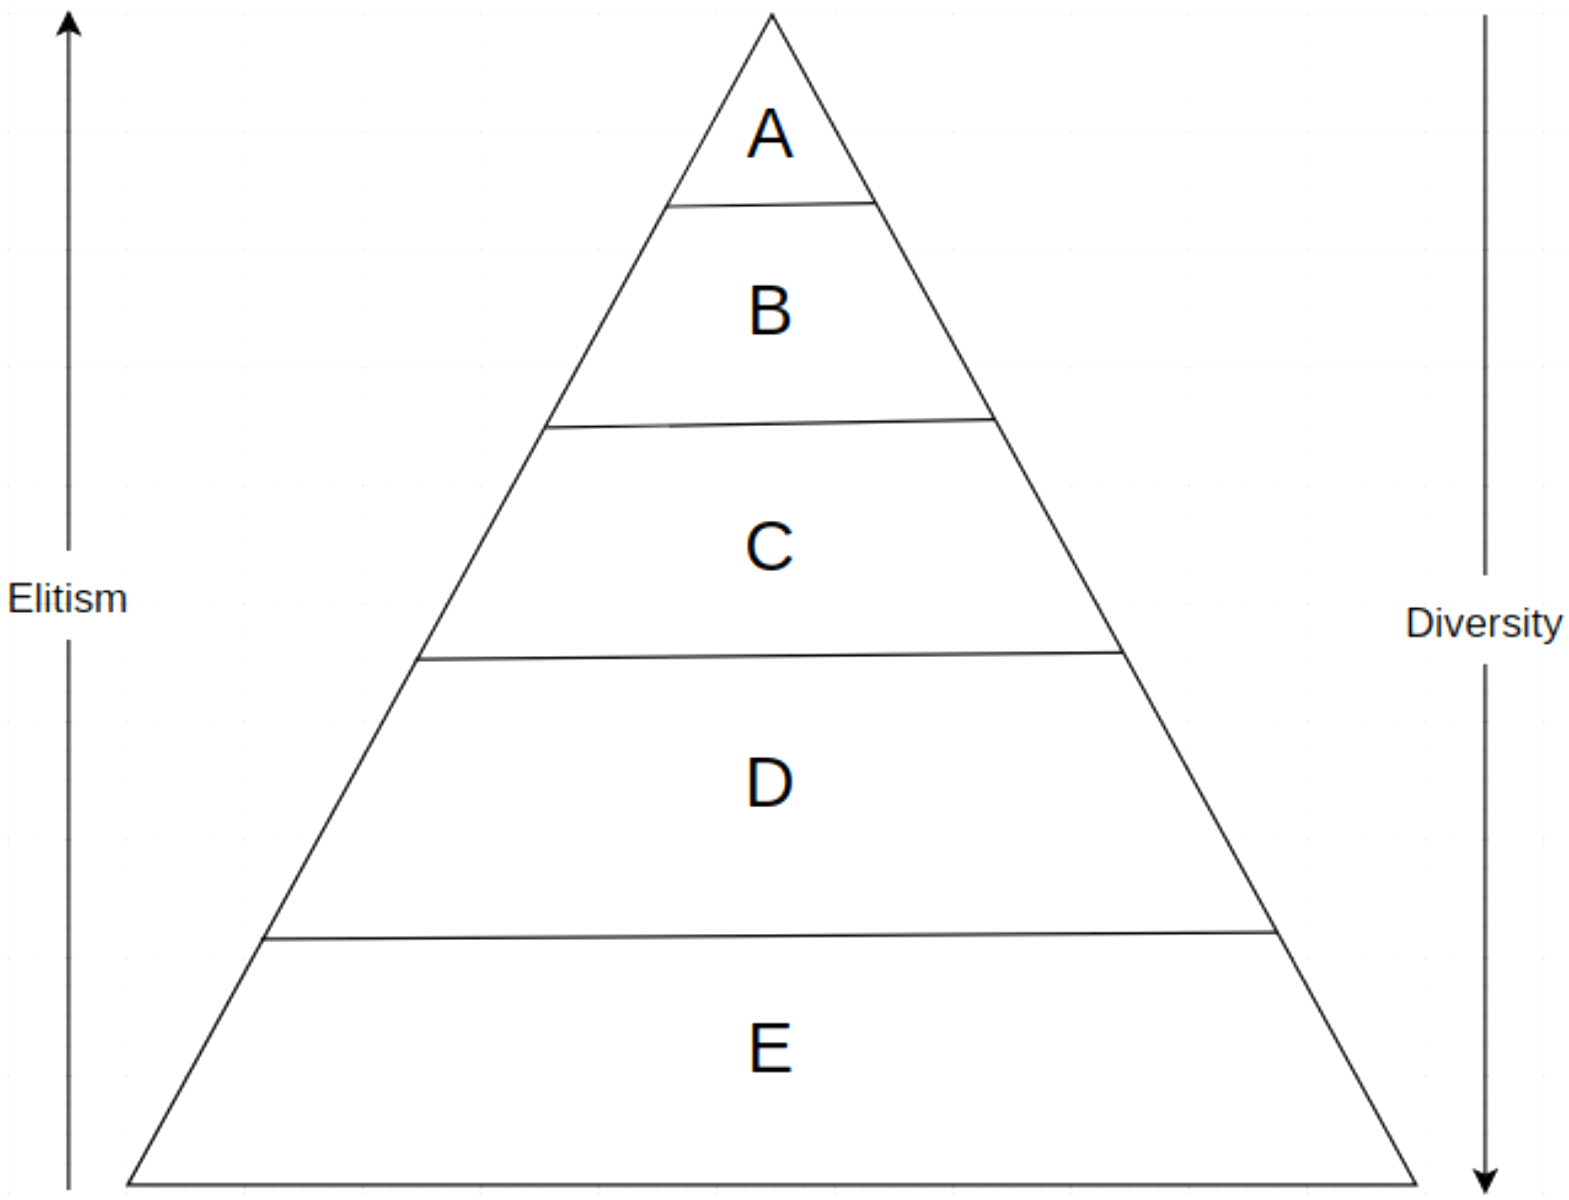
\includegraphics[height=5cm]{struct.png}
\caption{Structure of DA}
\label{struct}
\end{figure}

The division of departments is based on the relative scores obtained against the set fitness function. Candidates belonging to the higher departments dictate the overall global optima searching process whilst guiding and taking advice from the lower departments. Following initialization, there are two main seasons involved in this algorithm.
\begin{itemize}
\item Guiding Season
\item Voting Season
\end{itemize}

In the following subsections, models of the social hierarchy and the seasons are explained, followed by outlining of the entire algorithm.  

\subsection{Guiding Season}

This phase has the sole purpose of finding the optimal solution. Candidates belonging to the highest department are responsible for finding the solution. The other candidates act as advisers which help maintain the social structure and prevent the search process from falling into local optima. To introduce a dynamic factor in the search process, the solutions obtained by the top departments are continuously stored in a table for any future reference. The updation of the current position is done based on a weighted sum of the current position of all the departments. Based on the difference between the solution provided and the true solution, the top department's reward score is either incremented or decremented by 1. The algorithm is depicted in Algorithm $\ref{alg:gs}$.

\begin{algorithm}[!t]
\footnotesize
\caption{Guiding Season}
\label{alg:gs}
\begin{algorithmic}[1]
\STATE \textbf{Input:} Population size $\textit{n}$, Set of stopping criteria $\lambda\textsubscript{i}$, fitness function $\textit{f}$
\STATE Create candidate solutions $\textit{S}$ of size $\textit{n}$ 
\FOR{Each candidate $\textit{s\textsubscript{i}}$ in $\textit{S}$}
\STATE Apply $\textit{f}$ on $\textit{s\textsubscript{i}}$
\ENDFOR
\STATE Based on selected architecture, establish group dynamics
\WHILE{Any of $\lambda\textsubscript{i}$ are not met}
\IF{Predicted Fitness is acceptable}
\STATE Apply algorithms related to the selection phase
\ELSE
\STATE Apply algorithms related to the variation phase
\ENDIF
\ENDWHILE
\STATE Predicted solution corresponds to global optimum
\end{algorithmic}
\end{algorithm}

\subsection{Voting Season}

After a set period $\textit{T}$ if the total reward score does not exceed a threshold $\lambda$ then the top department is replaced by the one just below it. If $\lambda$ is exceeded, then the next problem is loaded with the current configuration.

The entire process of the voting season is displayed in Algorithm $\ref{alg:da}$.

\begin{algorithm}[!t]
\footnotesize
\caption{Voting Season}
\label{alg:da}
\begin{algorithmic}[1]
\STATE \textbf{Input:} Population size $\textit{n}$, random vector set $\vec{r\textsubscript{1,j}}$, $\vec{r\textsubscript{2,j}} \in$ [0,1], weight vector $\vec{w}$, initial estimate of global optimum $\textit{X\textsubscript{g}}$, time period $\textit{T}$, threshold $\lambda$, fitness function $\textit{f}$, coefficient vector sets $\vec{A\textsubscript{j}}$, $\vec{C\textsubscript{j}}$ and $\vec{a\textsubscript{j}}$
\STATE Set $\textit{t}$ = 0
\STATE Initialize vector set $\vec{A\textsubscript{j}}$ = 2$\vec{a} \cdot \vec{r\textsubscript{1}}$ - $\vec{a}$
\STATE Initialize vector set $\vec{C\textsubscript{j}}$ = 2$\vec{r\textsubscript{2}}$
% and $\vec{a\textsubscript{j}}$
\IF {Table $\textit{H}$ exists with current function problem}
\STATE Refer to table $\textit{H}$ for solution
\ELSE
\STATE Create table $\textit{H}$ mapping input to corresponding output and apply memoization
\STATE Create table $\textit{R}$ to store the performance of each department
\FOR{i $\in$ [1,n]}  
\STATE Generate population results $\textit{X\textsubscript{i}(t)}$ at instance $\textit{t}$
\STATE Evaluate each individual against the fitness function
\ENDFOR
\STATE Assign A, B, C, D, E departments as per the score against the fitness function. 
\STATE Evaluate $\vec{D\textsubscript{j}} = |\vec{C} \cdot \vec{X\textsubscript{g}}(t) - \vec{X\textsubscript{j}}(t)|$
\WHILE{t $<$ T}
\FOR{Each individual $\textit{X\textsubscript{i,j}(t)}$ in each department $\textit{j}$}
\STATE Update $\textit{X\textsubscript{i,j}(t)}$ := $\textit{X\textsubscript{j}(t)}$ - $\vec{A}$($\vec{D\textsubscript{j}}$)
\STATE $\textit{X\textsubscript{i,j}(t+1)}$ = $\frac{\vec{w} \cdot \textit{X\textsubscript{i,j}(t)}}{5}$
\ENDFOR
\STATE Check fitness of $\textit{X\textsubscript{top}}$ against $\textit{f}$
\IF{Fitness score is acceptable}
\STATE Increase score of $\textit{X\textsubscript{top}}$ in $\textit{R\textsubscript{top}}$ by 1
\ELSE
\STATE Decrease score of $\textit{X\textsubscript{top}}$ in $\textit{R\textsubscript{top}}$ by 1
\ENDIF
\ENDWHILE
\STATE At $\textit{t}$ = $\textit{T}$, check score of top department
\IF{$\textit{score\textsubscript{top}} \geq \lambda$}
\STATE Continue
\ELSE
\STATE Replace $\textit{X\textsubscript{top}}$ with $\textit{X\textsubscript{top-1}}$
\ENDIF
\STATE Update $\vec{a}$ := 2($\frac{T-t}{T}$)
\STATE Update $\vec{A}$ and $\vec{C}$ accordingly
\STATE $\textit{X\textsubscript{top}}$ represent required set of optimal solutions
\STATE Add corresponding function and solution to $\textit{H}$ for future reference
\ENDIF
\end{algorithmic}
\end{algorithm}

\subsection{Key points}

\begin{table*}
\caption{\textsc{Benchmark Functions}}
\label{tab:1}
\centering
\scalebox{0.9}
{
\begin{tabular}{| >{\arraybackslash}m{0.88in} | c | c | >{\arraybackslash}m{0.4in} | c | >{\arraybackslash}m{1in} | c |}
\hline
Function & ID & Formula & Modality & Range & Minimum Value & Department \\
\hline
Matyas & F1 & $0.26(x\textsubscript{2} + y\textsubscript{2}) - 0.48xy$ & Uni & [-10,10] & 0 at $x\textsuperscript{*}$ = (0,0) & A\\
Booth & F2 & $(x + 2y - 7)\textsuperscript{2} + (2x + y - 5)\textsuperscript{2}$ & Uni & [-10,10] & 0 at $x\textsuperscript{*}$ = (1,3) & A\\
Bohachevsky & F3 & $x\textsuperscript{2} + 2y\textsuperscript{2} -0.3cos(3\pi x)-0.4cos(4\pi y)+0.7$ & Uni & [-100,100] & 0 at $x\textsuperscript{*}$ = (0,0) & A\\
Gramacy and Lee & F4 & $\frac{sin(10\pi x)}{2x} + (x-1)\textsuperscript{4}$ & Uni & [-0.5,2.5] & -0.86 at $x\textsuperscript{*}$ = (0.54) & A\\
Leon & F5 & $100(y-x\textsuperscript{3})\textsuperscript{2}$ + $(1-x)\textsuperscript{2}$ & Uni & [-10,10] & 0 at $x\textsuperscript{*}$ = (1,1) & B\\
Ackley & F6 & $-20 exp(-0.2 \sqrt{\frac{1}{n} \sum_{i=1}^n x_i^2}) +$ e + & Multi & [-32,32] & 0 at $x\textsuperscript{*}$ = (0,0) & A\\
& &20 - $exp(\frac{1}{n} \sum_{i=1}^n cos(2\pi x_i))$&&&&\\
Bartels & F7 & $|x\textsuperscript{2} + y\textsuperscript{2} + xy| + |sin(x)| + |cos(y)|$ & Multi & [-500,500], [-500,500] & 1 at $x\textsuperscript{*}$ = (0,0) & A\\
Branin & F8 & $a(x\textsubscript{2} - bx\textsubscript{1}\textsuperscript{2} + cx\textsubscript{1} - r)\textsuperscript{2}$ + $s(1-t)cos(x\textsubscript{1})$ + s & Multi & [-5,10], [0,15] & 0.39 at $x\textsuperscript{*}$ = (-$\pi$, 12.275) & B\\
Egg Crate & F9 & $x\textsuperscript{2}$ + $y\textsuperscript{2}$ + $25(sin\textsuperscript{2}(x) + cos\textsuperscript{2}(x))$ & Multi & [-5,5] & 0 at $x\textsuperscript{*}$ = (0,0) & B\\
Qing & F10 & $\sum_{i=1}^{n}(x^2-i)^2$ & Multi & [-500,500] & 0 at $x\textsuperscript{*}$ = ($\pm\sqrt{i}$) & A\\
Rastrigin & F11 & $10n + \sum_{i=1}^{n}(x_i^2 - 10cos(2\pi x_i))$ & Multi & [-5.12,5.12], [-500,500] & 0 at $x\textsuperscript{*}$ = (0,0) & C\\
Rosenbrock & F12 & $\sum_{i=1}^{n}[b (x_{i+1} - x_i^2)^ 2 + (a - x_i)^2]$ & Multi & [-5.12,5.12], [-5,10] & 0 at $x\textsuperscript{*}$ = (1) & C\\
Bird & F13 & $sin(x)e\textsuperscript{(1-cos(y))\textsuperscript{2}}+cos(y)e\textsuperscript{(1-sin(x))\textsuperscript{2}}+(x-y)\textsuperscript{2}$ & Multi & [-2$\pi$, 2$\pi$] & -106.76 at $x\textsuperscript{*}$ = (4.70,3.15),(-1.58,-3.13) & A\\
Powell Sum & F14 & $\sum_{i=1}^{n}|x_i|^{i+1}$ & Multi & [-1,1] & 0 at $x\textsuperscript{*}$ = 0 & A\\
Schaffer & F15 & $0.5 + \frac{sin\textsuperscript{2}(x\textsuperscript{2}-y\textsuperscript{2})-0.5}{(1+0.001(x\textsuperscript{2}+x\textsuperscript{2}))\textsuperscript{2}}$ & Multi & [-100,100] & 0 at $x\textsuperscript{*}$ = (0,0) & B\\
Shubert & F16 & $\prod_{i=1}^{n}{\left(\sum_{j=1}^5{ cos((j+1)x_i+j)}\right)}$ & Multi & [-10,10] & -186.7309  & A\\
Happy Cat & F17 & $\left[\left(||\textbf{x}||^2 - n\right)^2\right]^\alpha + \frac{1}{n}\left(\frac{1}{2}||\textbf{x}||^2+\sum_{i=1}^{n}x_i\right)+\frac{1}{2}$ & Multi & [-2,2] & 0 at $x\textsuperscript{*}$ = (-1)  & A\\
Alpine & F18 & $\prod_{i=1}^{n}\sqrt{x_i}sin(x_i)$ & Multi & [0,10] & 2.80 at $x\textsuperscript{*}$ = (7.91)  & B\\
\hline
\end{tabular}
}
\end{table*}

DA is a subset of Multi-Objective Evolutionary Algorithms and follows a similar convergence proof with slight modifications as proposed by G. Rudolph and A. Agapie \cite{conv}. He related the choice of evolutionary operations to the positiveness of a variation kernel. If the transition probability from a set of chromosomes to any solution is non-zero positive, then the transition process of the operations have a positive variation kernel. Extending this across with a homogeneous Markov chain having a positive transition matrix, it has been proven the all Pareto-optimal solutions will be the global solution in finite time with probability one. To prove the stochastic convergence, we first need to define a measure for the mapping.

\begin{theorem}
If $A$ and $B$ are subsets of a finite population set $X$ the $d(A,B)$ = $|A \cup B| - |A \cap B|$ is a metric on the power set of $X$
\end{theorem}

\begin{proof}\renewcommand{\qedsymbol}{}
Let $X$ = $\{X\textsuperscript{1}, X\textsuperscript{2} \dots, X\textsuperscript{n} \}$ be the candidates and $a\textsubscript{i}$ and $b\textsubscript{i}$ be the candidate and solution incidence vectors. \\
{\scriptsize
\begin{align*}
d(A,B) &= \sum_{i=1}^{n}(a\textsubscript{i} + b\textsubscript{i} - 2a\textsubscript{i}b\textsubscript{i})\\
 &= \sum_{i=1}^{n}[(1-b\textsubscript{i})a\textsubscript{i} + (1-a\textsubscript{i})b\textsubscript{i}]\\
 &= \sum_{i=1}^{n}|a\textsubscript{i} - b\textsubscript{i}| = ||a - b||\textsubscript{1}
\end{align*}
}
\end{proof}
Therefore the Hamming Distance between the incidence vectors can act as a metric for mapping. A secondary measure utilized in the mapping is $\delta\textsubscript{B}(A)$ = $|A| - |A \cap B|$ which counts the number of candidates in set $A$ but not in set $B$. Stochastic convergence proof is discussed next. 

\begin{theorem}
Let $n\textsubscript{t}$ be the population of DA at time $t \geq 0$ and $F\textsubscript{t} = f(n\textsubscript{t})$ be the optimal mapping. DA is said to converge at probability 1 to the entire set if
{\scriptsize
\begin{equation*}
d(F\textsubscript{t}, M\textsuperscript{*}) \rightarrow 0,  t \rightarrow \infty
\end{equation*}
}
where convergence to set of minimal elements $\textit{M\textsuperscript{*}}$ occurs at probability 1 if 
{\scriptsize
\begin{equation*}
\delta\textsubscript{M\textsuperscript{*}}(F\textsubscript{t}) \rightarrow 0\\
\end{equation*}
}
with probability 1 as $\textit{t} \rightarrow \infty$
\end{theorem}

The implication of $d(F\textsubscript{t}, M\textsuperscript{*}) \rightarrow 0$ implies $\delta\textsubscript{M\textsuperscript{*}}(F\textsubscript{t}) \rightarrow 0$ extends to the worst case scenario of $n = M\textsuperscript{*}$. However, if a Markov Chain is maintained dynamically, $|M\textsuperscript{*}|=1$ and the limited population size will converge to a critical point. The rate of convergence is another important piece in this discussion. 

\begin{theorem}
Let $n\textsubscript{i,t}$, $F$, $GM$ and $\lambda$ be the population of the $i\textsuperscript{th}$ department of DA at time $t$, fitness function, rate of cross-over-mutation and threshold for the memory element respectively. The rate of population progression from department $i$ to $j$ for a given problem can be expressed as
{\scriptsize
\begin{equation*}
\frac{d(Population\textsubscript{i $\rightarrow$ j})}{dt} \propto f(n\textsubscript{i,t}, \frac{1}{F}, GM, \lambda)
\end{equation*}
}
\end{theorem}

\begin{proof}\renewcommand{\qedsymbol}{}

Consider $n\textsubscript{i,t}$ and $F$ as a combined quantity $Q(i,j,t)$. The distribution of $Q(i,j,t)$ will be binomial as the peak is achived with maximum population and highest fitness score. The probability of candidate $c$ at department $i$ to continue into department $j$ at time $t+1$ will be given by
{\scriptsize
\begin{equation*}
P(j|i,t+1) =  {n\textsubscript{$i$,$t$} \choose n\textsubscript{$i$,$t$}} GM\textsuperscript{$n\textsubscript{$i$,$t$}$}
\end{equation*}
}



Based on this distribution, diffusion equations with initial state $p$, relative frequency of candidate selection till current department $\mu$ and selection strength $s$ can be written as:
{\scriptsize
\begin{equation*}
\frac{\partial \mu(p,t)}{\partial t} = \frac{p(1-p)}{2}\frac{\partial^2 \mu(p,t)}{\partial^2 p} + sp(1-p)\frac{\partial mu(p,t)}{\partial mu}
\end{equation*}
}
Fixing this probability when $t$ $\rightarrow$ $\infty$ as
{\scriptsize
\begin{equation*}
u(p) = \lim_{t \rightarrow \infty} {\partial(p,t)}
\end{equation*}
}
We get the rate of transition of a candidate as a function of the proficiency over time $t$, $u(p)\textsuperscript{$t$}$.
\end{proof}
% From a mathematical point of view, both the structure and the search processes evolve over time with feedback. For each search, a lookup is conducted by candidate $\textit{c}$ in table $\textit{H}$. If not found, a solution $\textit{x\textsubscript{0}}$ is assumed as the initial point and the search of optimum solution $\textit{x\textsubscript{1}}$ begins. At the end of each expedition, the top department's performance is graded through a reward system. Based on the global performance overall a set runtime, either the department continues in power or gets replaced.

Based on the representation, the following observations can be made:
\begin{itemize}
\item The updation process occurs at an individual and at a departmental level to save the best solutions obtained so far
\item The parameters $\vec{A}$ and $\vec{C}$ assist the solutions to have higher dimensionality
\item Due to the dual updation and introduction of a memory element, the problems functions will saturate at a middle level department
\item The voting season provides weighted rights to each candidate in each department. The weights are assigned based on the individual's fitness which in turn is dependent on their department's position 
\item As the department rank increases, the number of individual candidate in the department decreases to promote elitism. This would ensure survival of the best solutions in future problems. 
\item As the department rank decreases, the number of individual candidate in the department increase to promote diversity. This would open up new avenues to explore and possibly increase chances of finding the gobal optimum.  
\item The increased number of parameters requires fine tunning which can be automated
\end{itemize}

To sum up, DA starts with generating and evaluating a set of candidate solutions. The solutions are grouped according to their relative goodness of fit. The top candidates are responsible for finding the optimum solution while the other candidates are required to maintain the hierarchy, provide valuable input to the leaders, and contest when the results begin deteriorating. When the top department does not function as per requirement, the lower departments replace it. A memory component is introduced in the form of a table that maps the previously encountered inputs to their corresponding outputs. 



\section{Results and Discussion}

In this section, the DA algorithm is benchmarked against 18 standard minimization functions. These functions are described in Table $\ref{tab:1}$. The DA  iterated 20 times on each of these functions and the results were compared against other popular SI algorithms such as Particle Swarm Optimization (PSO) \cite{pso}, Grey Wolf Optimization (GWO) \cite{gwo}, Multiverse Optimization (MVO)\cite{mvo} and Cuckoo Search (CS) \cite{cs}. The experiment was set up on a 64-bit Machine with Ubuntu 20.04, Intel® CoreTM i5-7200U CPU @ 2.50GHz × 4, with a GeForce 940MX/PCle/SSE2 graphic card.

DA provides ambitious results on the standard benchmark functions \cite{bf}. DA outperforms the other algorithms in F2, F8, F15, and F18. The selective performance boosts could be attributed to the optimal voting season. In certain cases, the top departments would have saturated and the replacement process might have been ineffective. As it is the case with any algorithm, the global optimum search can never be guaranteed. The critical point discussed in the previous section is Department C based on the experimental runs conducted. The results have been listed in Table $\ref{tab:2}$.

\begin{table*}
\scriptsize
\caption{\textsc{Benchmark Results}}
\label{tab:2}
\centering
{
\begin{tabular}{| c | c  c | c  c | c  c | c  c | c  c |}
\hline
{\textbf{Function}}&{\textbf{PSO}}&{}&{\textbf{GWO}}&{}&{\textbf{MVO}}&{}&{\textbf{CS}}&{}&{\textbf{DA}}&{}\\
\hline
{}&{\textbf{Mean}}&{\textbf{Std}}&{\textbf{Mean}}&{\textbf{Std}}&{\textbf{Mean}}&{\textbf{Std}}&{\textbf{Mean}}&{\textbf{Std}}&{\textbf{Mean}}&{\textbf{Std}}\\
\hline
{F1}&{1.339E-08}&{6.224E-04}&{2.411E-06}&{4.968E-05}&{5.221E-06}&{8.235E-08}&{9.711E-06}&{4.397E-07}&{8.712E-06}&{5.113E-05}\\
{F2}&{4.859E-10}&{0.5287}&{6.276E-09}&{5.171E-06}&{6.181E-07}&{0.8412}&{9.551E-09}&{3.854E-07}&{7.622E-11}&{2.625E-06}\\
{F3}&{8.156E-13}&{1.712E-07}&{3.897E-11}&{8.422E-07}&{9.252E-15}&{4.976E-06}&{2.416E-12}&{8.256E-07}&{1.823E-15}&{7.424E-05}\\
{F4}&{-0.7624}&{3.153}&{-0.6887}&{18.542}&{-0.8219}&{12.843}&{-0.7943}&{28.954}&{-0.8149}&{21.148}\\
{F5}&{0}&{0.0133}&{5.18E-24}&{0.0023}&{4.81E-20}&{0.0141}&{5.73E-27}&{0.0072}&{8.19E-29}&{0.0058}\\
{F6}&{5.177E-16}&{0.0251}&{1.415E-11}&{0.0595}&{2.478E-38}&{0.0224}&{7.714E-24}&{0.0119}&{4.082E-32}&{0.0084}\\
{F7}&{0.9521}&{0.0253}&{0.8445}&{0.0081}&{0.5122}&{0.0047}&{0.9154}&{0.0005}&{0.9204}&{0.0007}\\
{F8}&{0.3181}&{0.0012}&{0.2118}&{0.0084}&{0.3518}&{0.0152}&{0.3154}&{0.0002}&{0.3751}&{0.0084}\\
{F9}&{1.145E-08}&{5.152E-06}&{1.845E-09}&{5.691E-05}&{4.845E-08}&{3.452E-06}&{7.183E-08}&{6.541E-07}&{2.495E-09}&{5.88E-06}\\
{F10}&{5.483E-19}&{4.465E-08}&{7.842E-18}&{9.421E-05}&{7.515E-25}&{4.118E-05}&{9.152E-19}&{4.783E-05}&{1.215E-19}&{2.512E-06}\\
{F11}&{6.152E-20}&{0.0512}&{4.125E-38}&{0.0001}&{2.489E-28}&{0.0915}&{4.852E-26}&{0.0185}&{4.845E-29}&{0.0943}\\
{F12}&{0.0051}&{0.0218}&{0.0009}&{0.3512}&{0.0205}&{0.0945}&{0.0006}&{0.1534}&{0.001}&{0.0035}\\
{F13}&{-100.15}&{0.0029}&{-98.153}&{0.0675}&{-63.156}&{0.0005}&{-156.51}&{0.0266}&{-94.845}&{0.432}\\
{F14}&{0.0241}&{0.0008}&{0.0099}&{0.0021}&{0.0007}&{0.0315}&{0.0842}&{0.0239}&{0.0579}&{0.0679}\\
{F15}&{5.194E-16}&{8.495E-05}&{7.162E-20}&{2.846E-05}&{7.899E-E11}&{3.793E-05}&{6.977E-19}&{8.297E-05}&{3.842E-22}&{2.655E-07}\\
{F16}&{-215.15}&{0.0021}&{-288.31}&{0.0842}&{-160.249}&{0.3512}&{-206.49}&{0.0002}&{-153.123}&{0.0004}\\
{F17}&{0.0021}&{0.1532}&{0.0044}&{0.2953}&{0.0531}&{0.0212}&{0.0094}&{0.0121}&{0.0076}&{0.4683}\\
{F18}&{2.5321}&{0.0515}&{1.2854}&{0.7542}&{1.9458}&{0.1523}&{2.0057}&{0.0021}&{2.6185}&{0.0218}\\
\hline
\end{tabular}
}
\end{table*}

The plots for F1, F2, F3, F6, F15 and F17 have been shown in Figures $\ref{fig:figur:1}$, $\ref{fig:figur:2}$, $\ref{fig:figur:3}$, $\ref{fig:figur:4}$, $\ref{fig:figur:5}$ and $\ref{fig:figur:6}$. For these functions, the initial top department was capable of producing acceptable results. Due to the acceptance, the voting season never arrived and the process terminated. 


The plots for F8, F10 and F18 have been shown in Figures $\ref{fig:figur:7}$, $\ref{fig:figur:8}$, $\ref{fig:figur:9}$, $\ref{fig:figur:10}$, $\ref{fig:figur:11}$ and $\ref{fig:figur:12}$. For these two functions, the initial top department was inapable of producing acceptable results. In the following voting season the total reward did not exceed $\lambda$ and hence B dominance started. 

The plots for F11 and F12 have been shown in Figures $\ref{fig:figur:13}$, $\ref{fig:figur:14}$, $\ref{fig:figur:15}$, $\ref{fig:figur:16}$, $\ref{fig:figur:17}$ and $\ref{fig:figur:18}$. For these two functions, both, the initial top department and the subsequent leaders, were incapable of producing acceptable results. Due to the acceptance, the top departments were voted out after two voting seasons. Department C is promoted and it performs better due to the improved structure and the experience accumulated by the previous top departments.\\
% 

% The plots for F8, F10 and F18 have been shown in Figures $\ref{figur:7}$, $\ref{figur:8}$, $\ref{figur:9}$, $\ref{figur:10}$, $\ref{figur:11}$ and $\ref{figur:12}$. For these two functions, the initial top department was inapable of producing acceptable results. In the following voting season the total reward did not exceed $\lambda$ and hence B dominance started. 
% 
% The plots for F11 and F12 have been shown in Figures $\ref{figur:13}$, $\ref{figur:14}$, $\ref{figur:15}$, $\ref{figur:16}$, $\ref{figur:17}$ and $\ref{figur:18}$. For these two functions, both, the initial top department and the subsequent leaders, were incapable of producing acceptable results. Due to the acceptance, the top departments were voted out after two voting seasons. Department C is promoted and it performs better due to the improved structure and the experience accumulated by the previous top departments.\\
% % 
% \begin{figure}[!t]
% \subfloat[Branin-A]{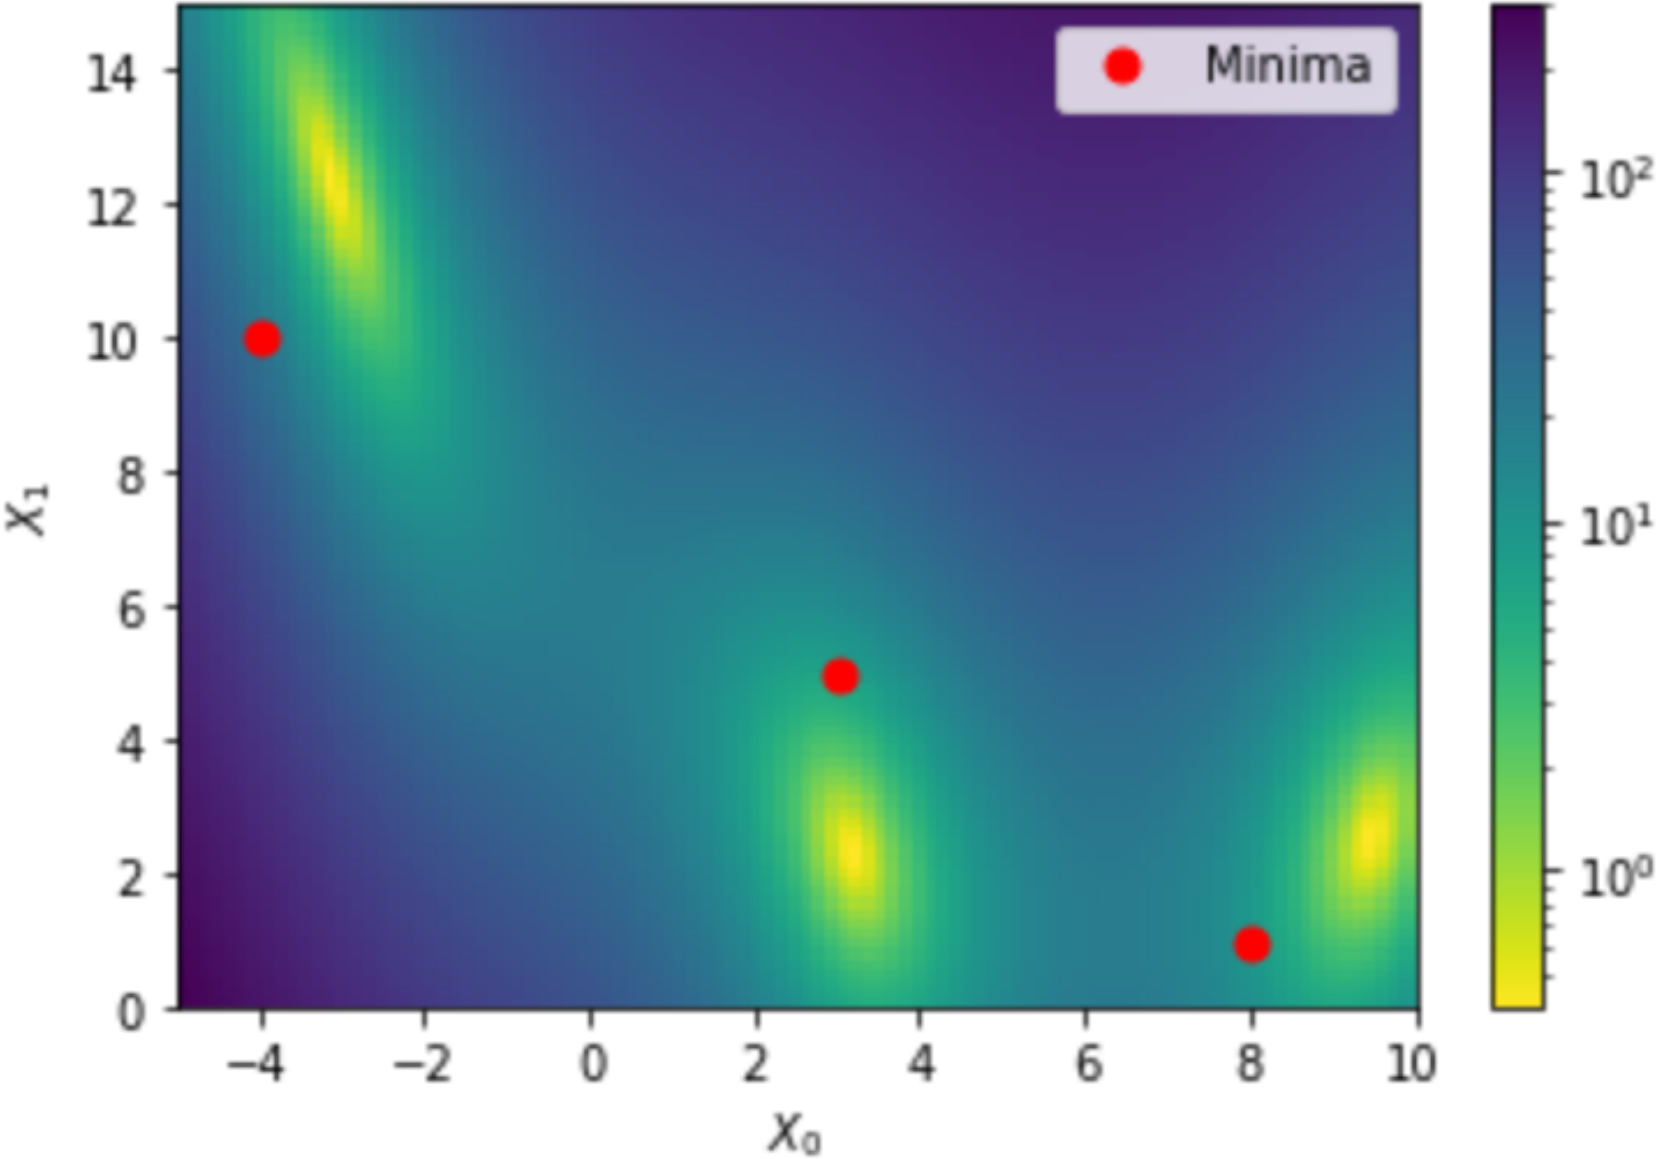
\includegraphics[width = 2in]{branina.png}} 
% \subfloat[Branin-B]{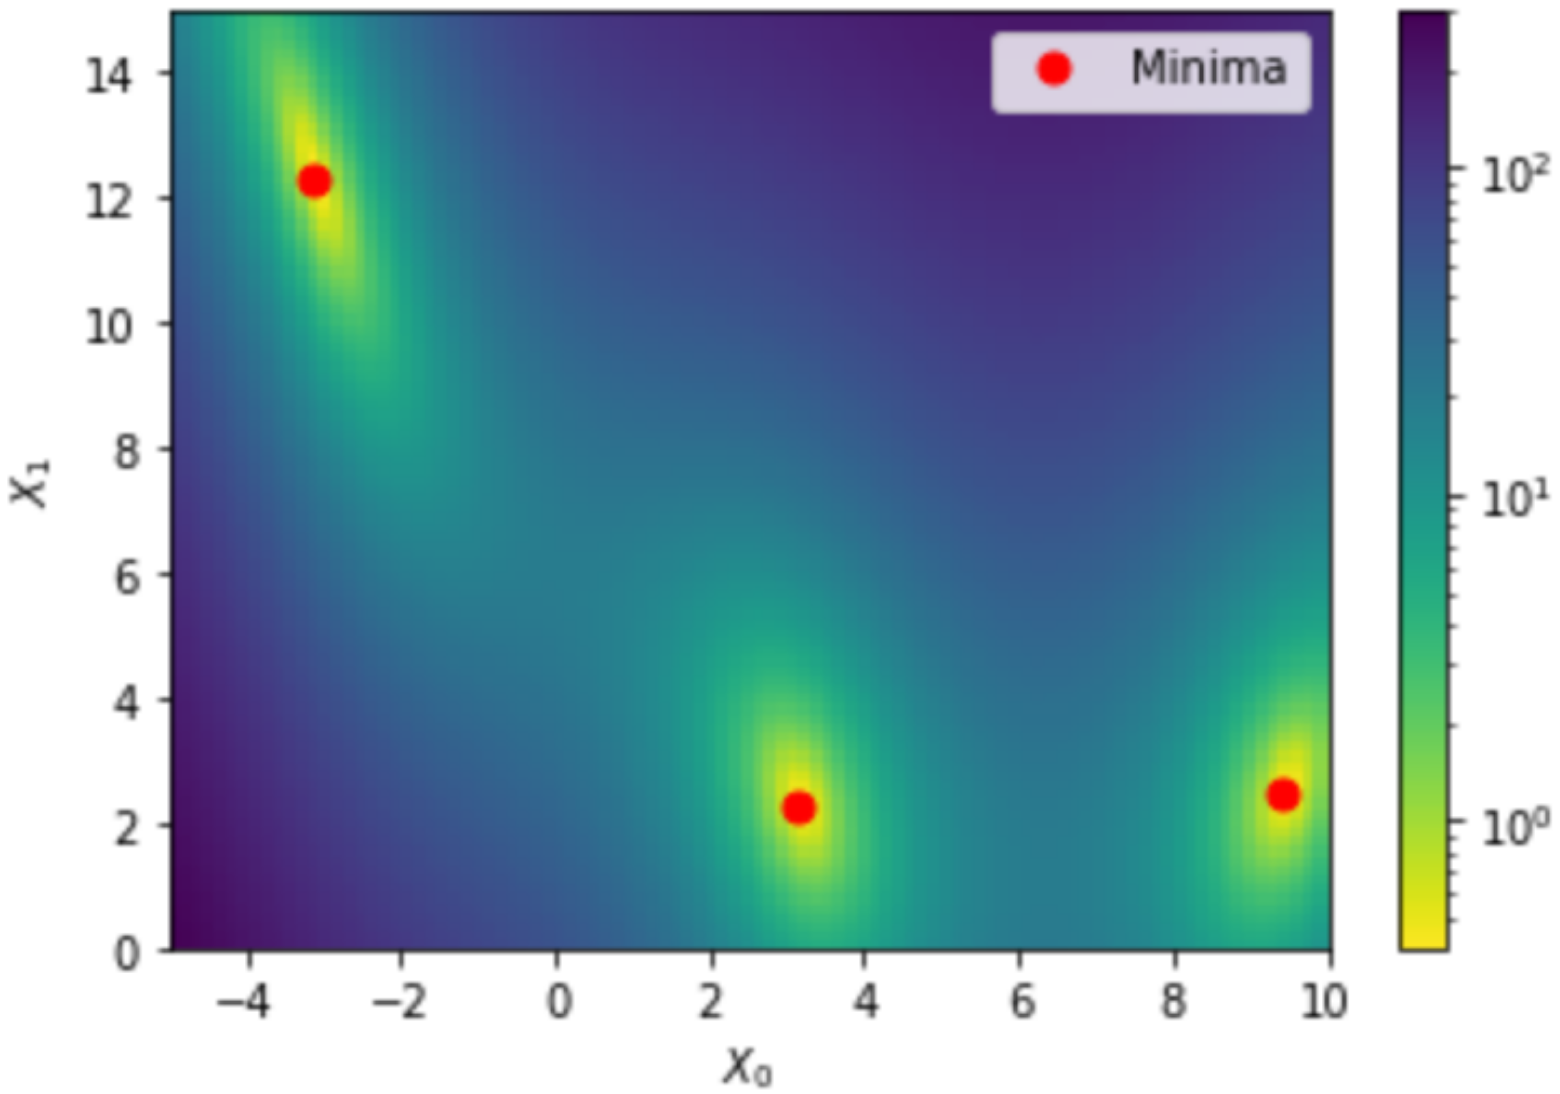
\includegraphics[width = 1.9in]{braninb.png}}\\
% \caption{}
% \label{fig:sfig3}
% \end{figure}
% \begin{figure}[!t]
% \begin{subfigure}{.275\textwidth}
%   \centering
%   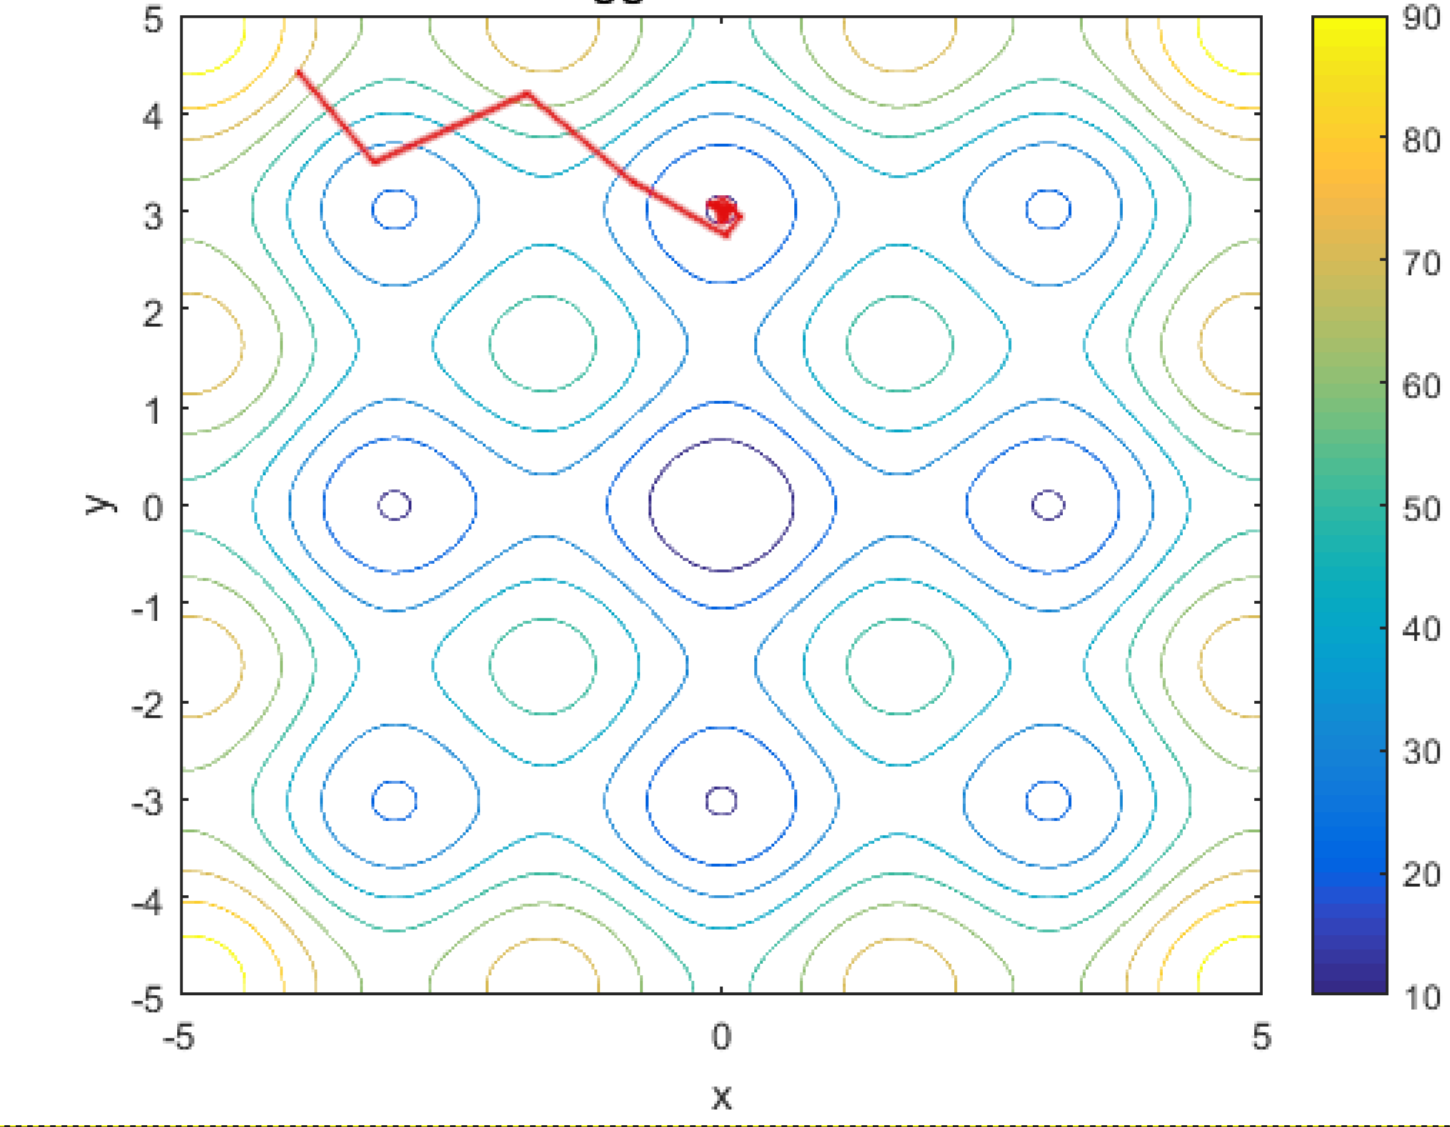
\includegraphics[width=.8\linewidth]{egga.png}
%   \caption{Egg Crate-A}
%   \label{fig:sfig4}
% \end{subfigure}%
% \begin{subfigure}{.275\textwidth}
%   \centering
%   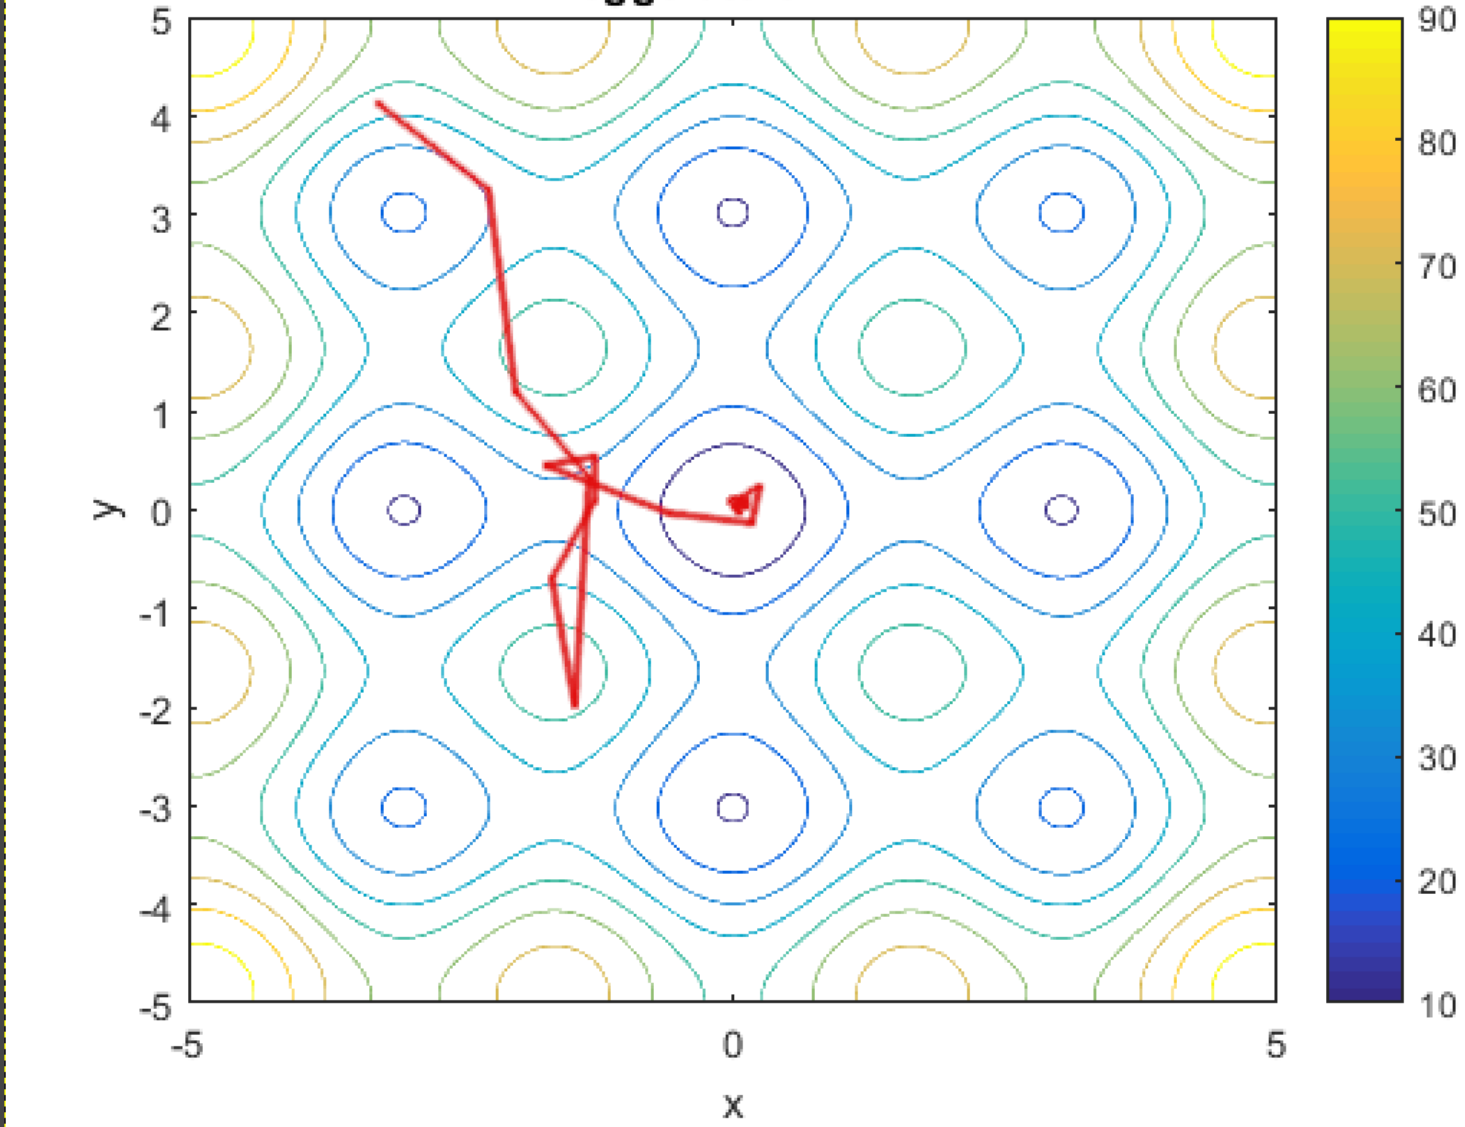
\includegraphics[width=.8\linewidth]{eggb.png}
%   \caption{Egg Crate-B}
%   \label{fig:sfig5}
% \end{subfigure}
% \caption{Departmant B Dominance}
% \label{fig:sfig6}
% \end{figure}
% 
% The plots for F11 and F12 have been shown in Figures $\ref{fig:sfig7}$ and $\ref{fig:sfig8}$. For these two functions, both, the initial top department and the subsequent leaders, were incapable of producing acceptable results. Due to the acceptance, the top departments were voted out after two voting seasons. Department C is promoted and it performs better due to the improved structure and the experience accumulated by the previous top departments.
% 
% \begin{figure}[!t]
% \subfloat[Rastrigin-A]{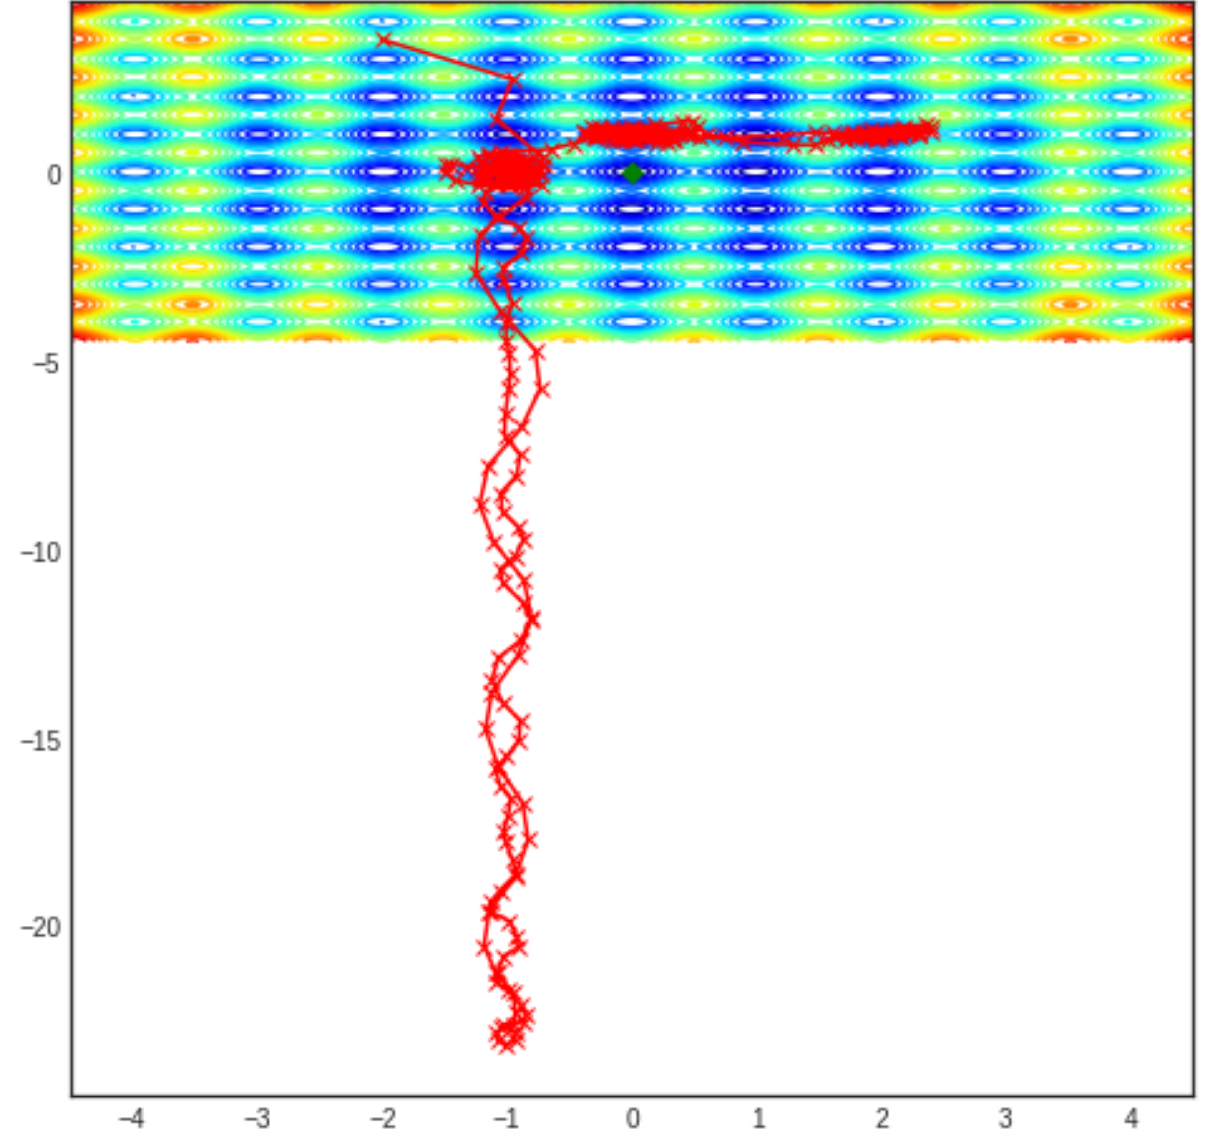
\includegraphics[width = 1.25in]{rastrigina.png}} 
% \subfloat[Rastrigin-B]{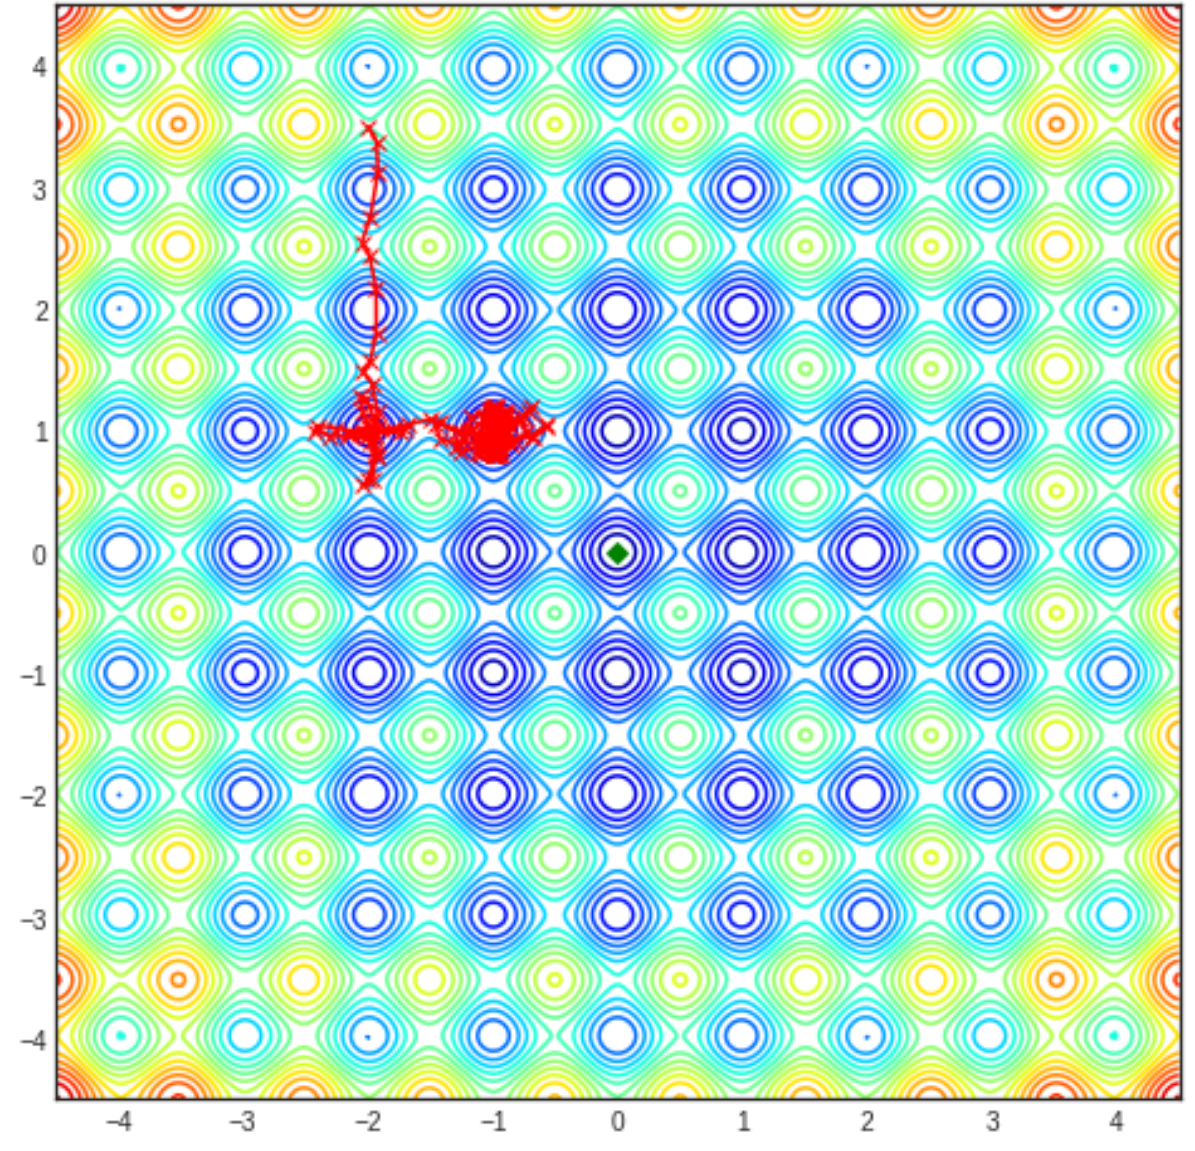
\includegraphics[width = 1.25in]{rastriginb.png}}
% \subfloat[Rastrigin-C]{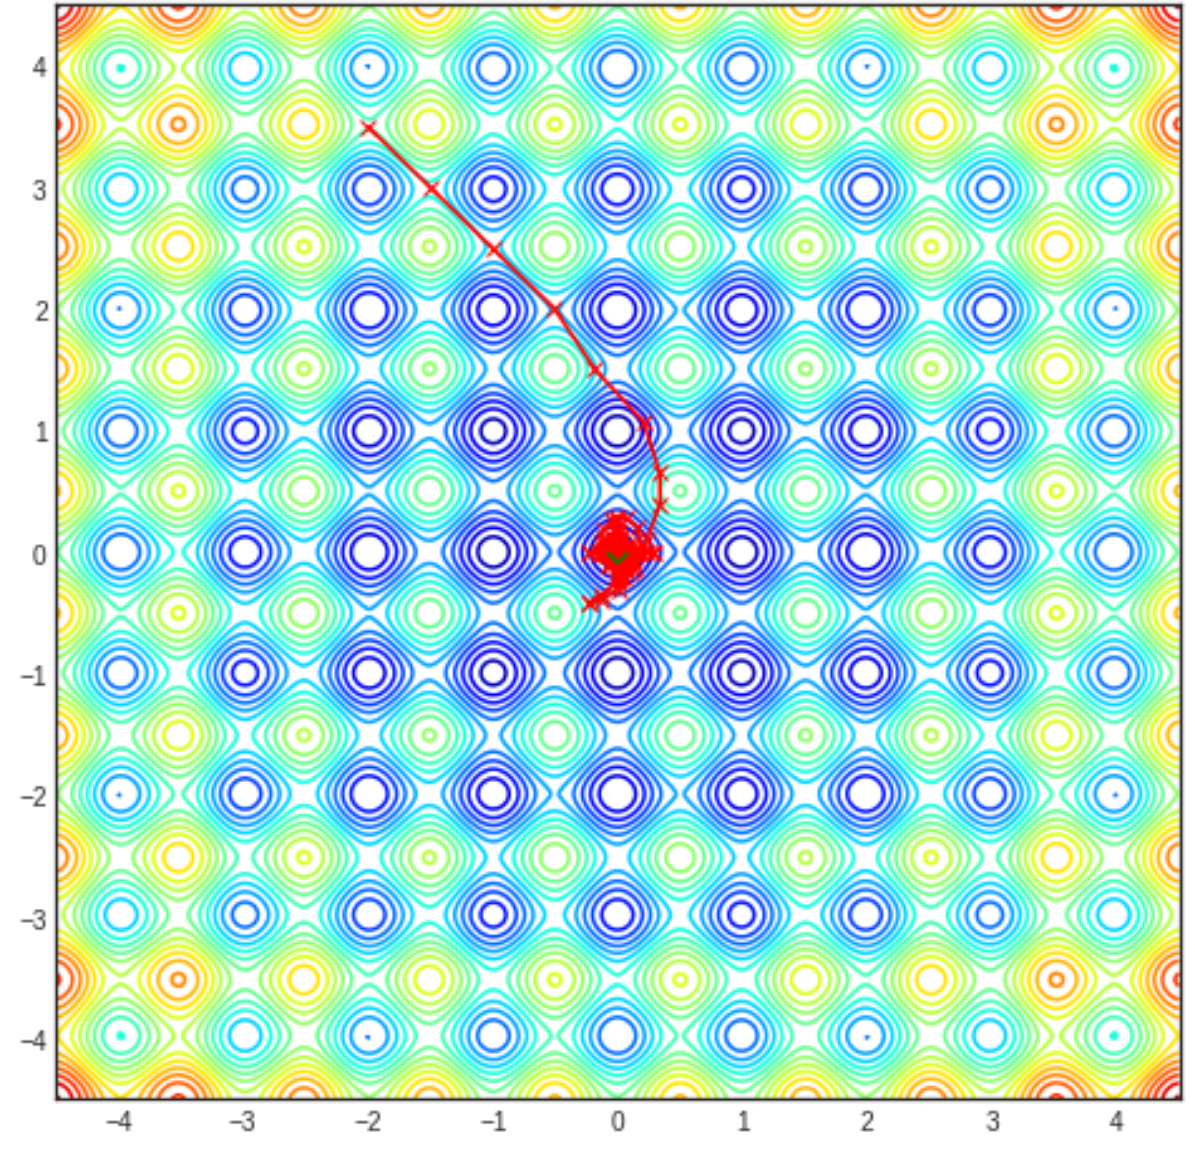
\includegraphics[width = 1.25in]{rastriginc.png}}\\
% \caption{}
% \label{fig:sfig7}
% \end{figure}
% 
% \begin{figure}[!t]
% \subfloat[Rosenbrock-A]{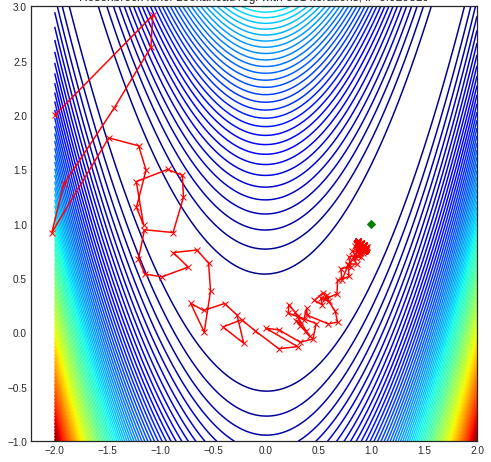
\includegraphics[width = 1.25in]{rosenbrocka.png}} 
% \subfloat[Rosenbrock-B]{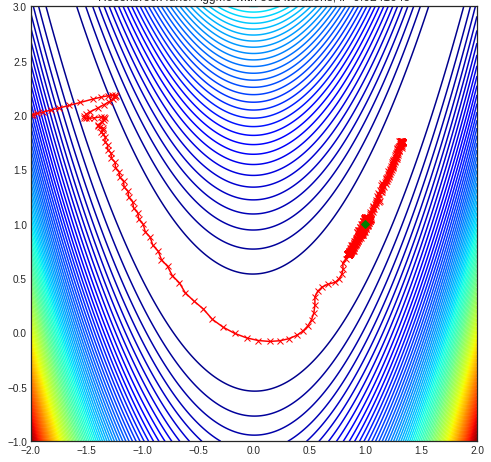
\includegraphics[width = 1.25in]{rosenbrockb.png}}
% \subfloat[Rosenbrock-C]{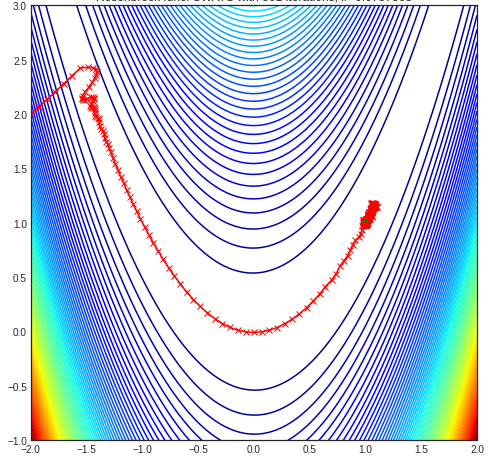
\includegraphics[width = 1.25in]{rosenbrockc.png}}\\
% \caption{Department C Dominance}
% \label{fig:sfig8}
% \end{figure}

\begin{figure}[htp]
\begin{subfigure}{.275\textwidth}
  \centering
  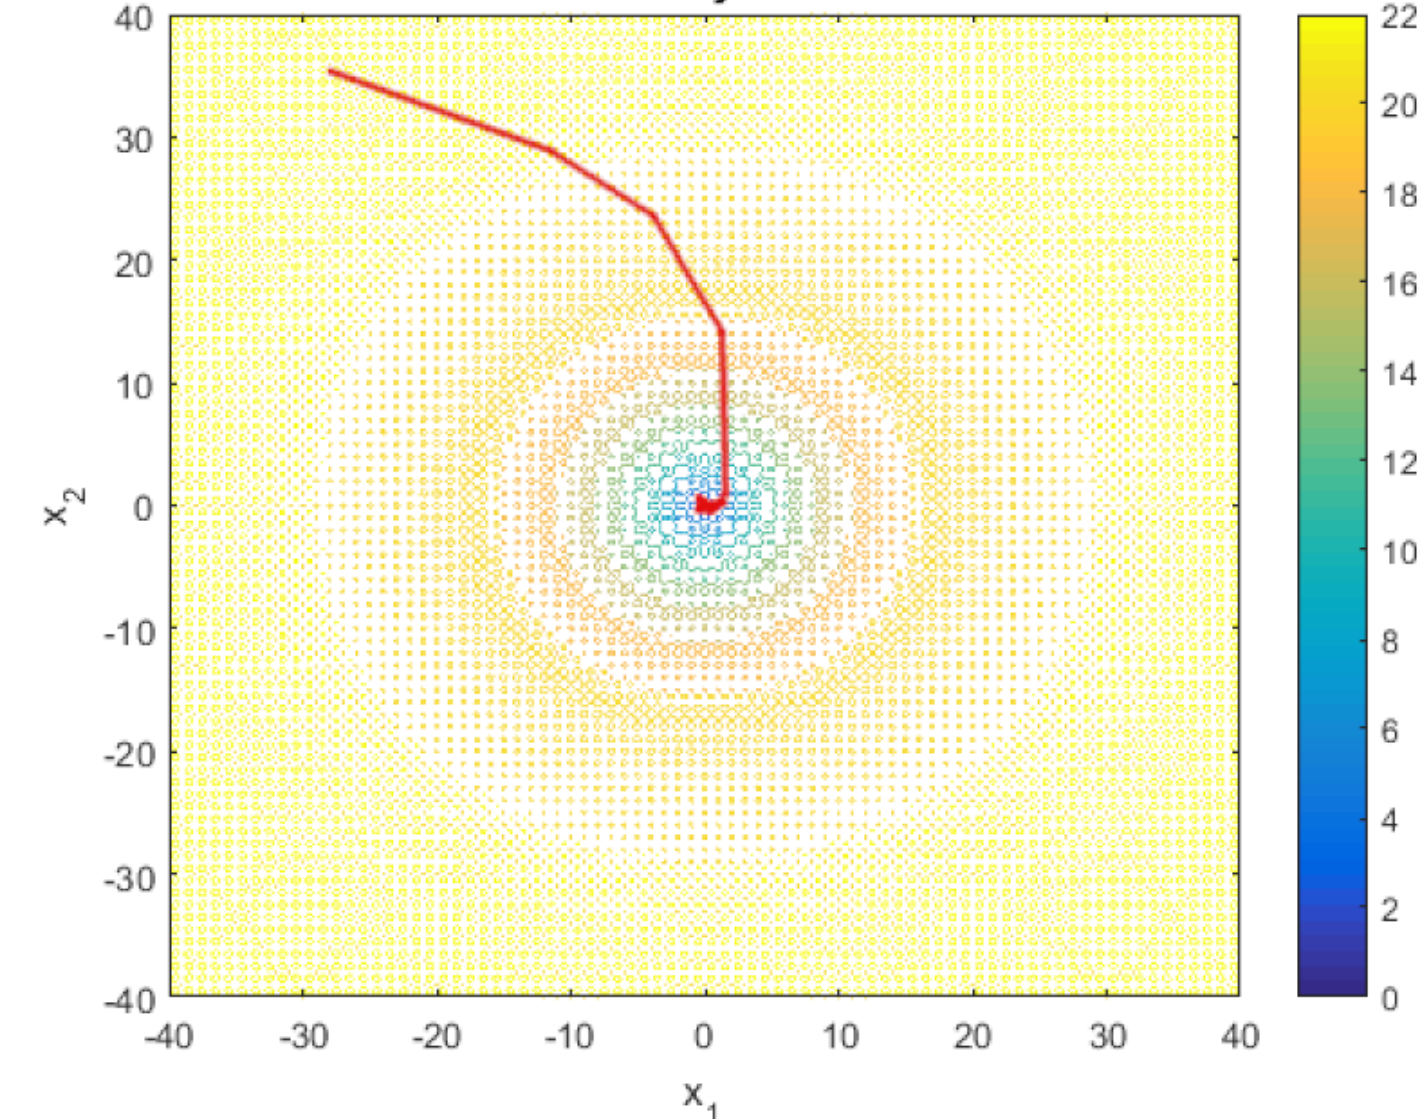
\includegraphics[width=.6\linewidth]{ackley.png}
  \caption{Ackley}
  \label{fig:figur:1}
\end{subfigure}%
\begin{subfigure}{.275\textwidth}
  \centering
  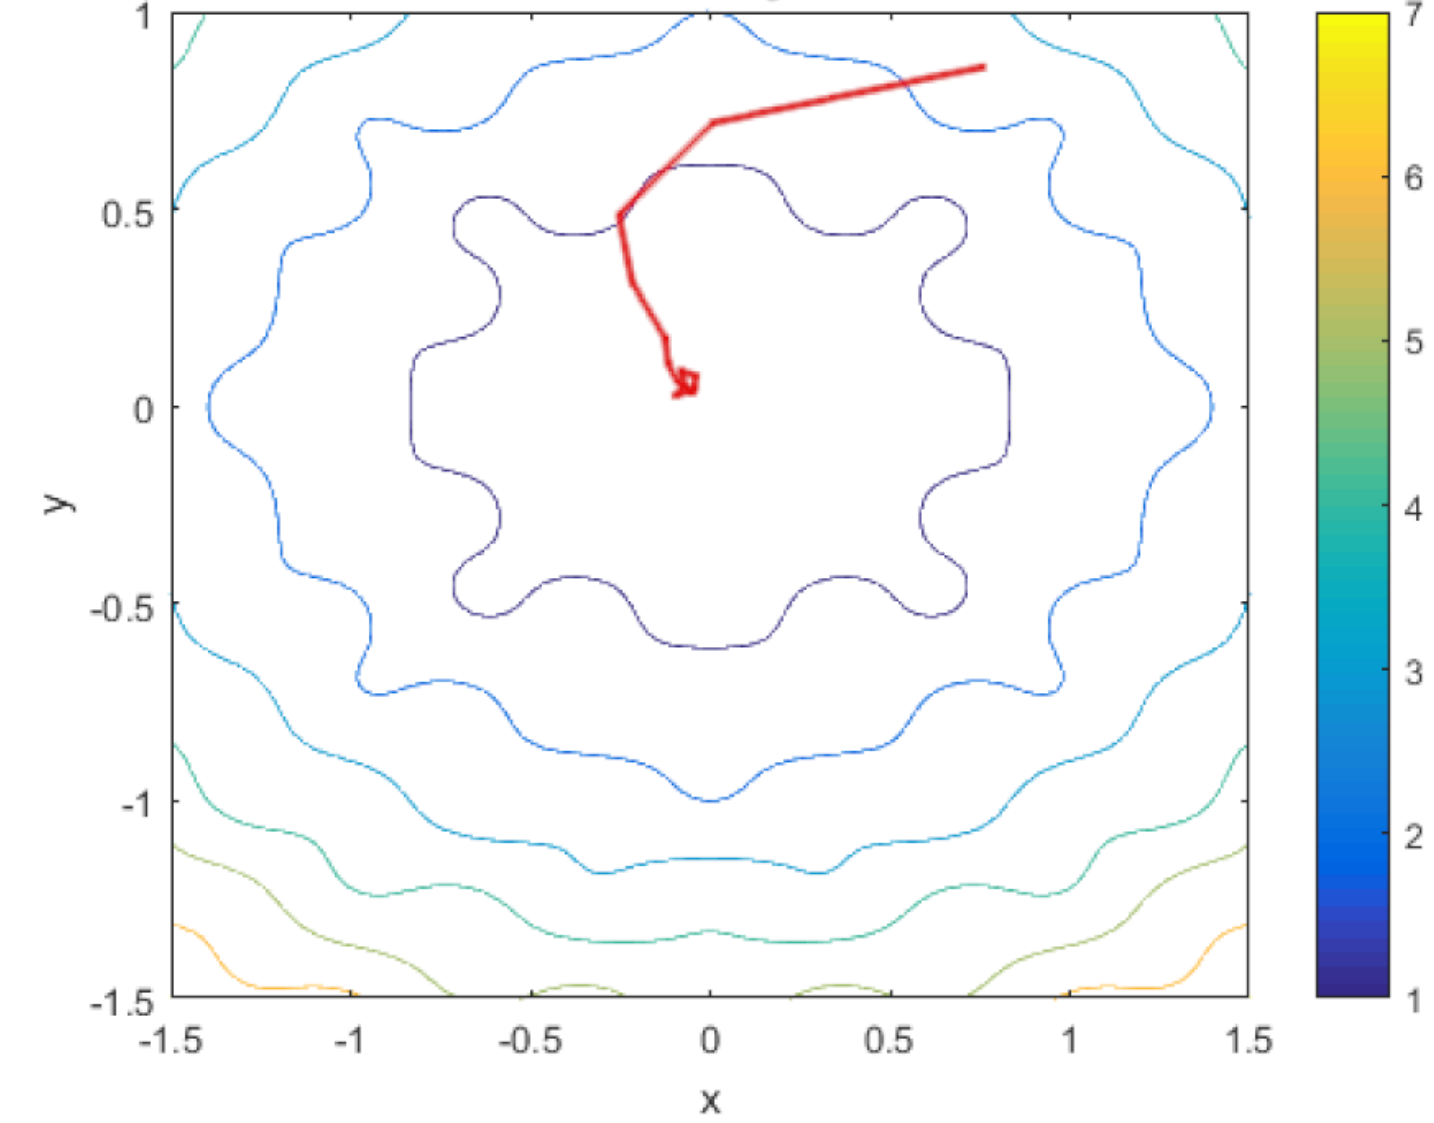
\includegraphics[width=.6\linewidth]{boha.png}
  \caption{Bohachevskyn}
  \label{fig:figur:2}
\end{subfigure}
\begin{subfigure}{.275\textwidth}
  \centering
  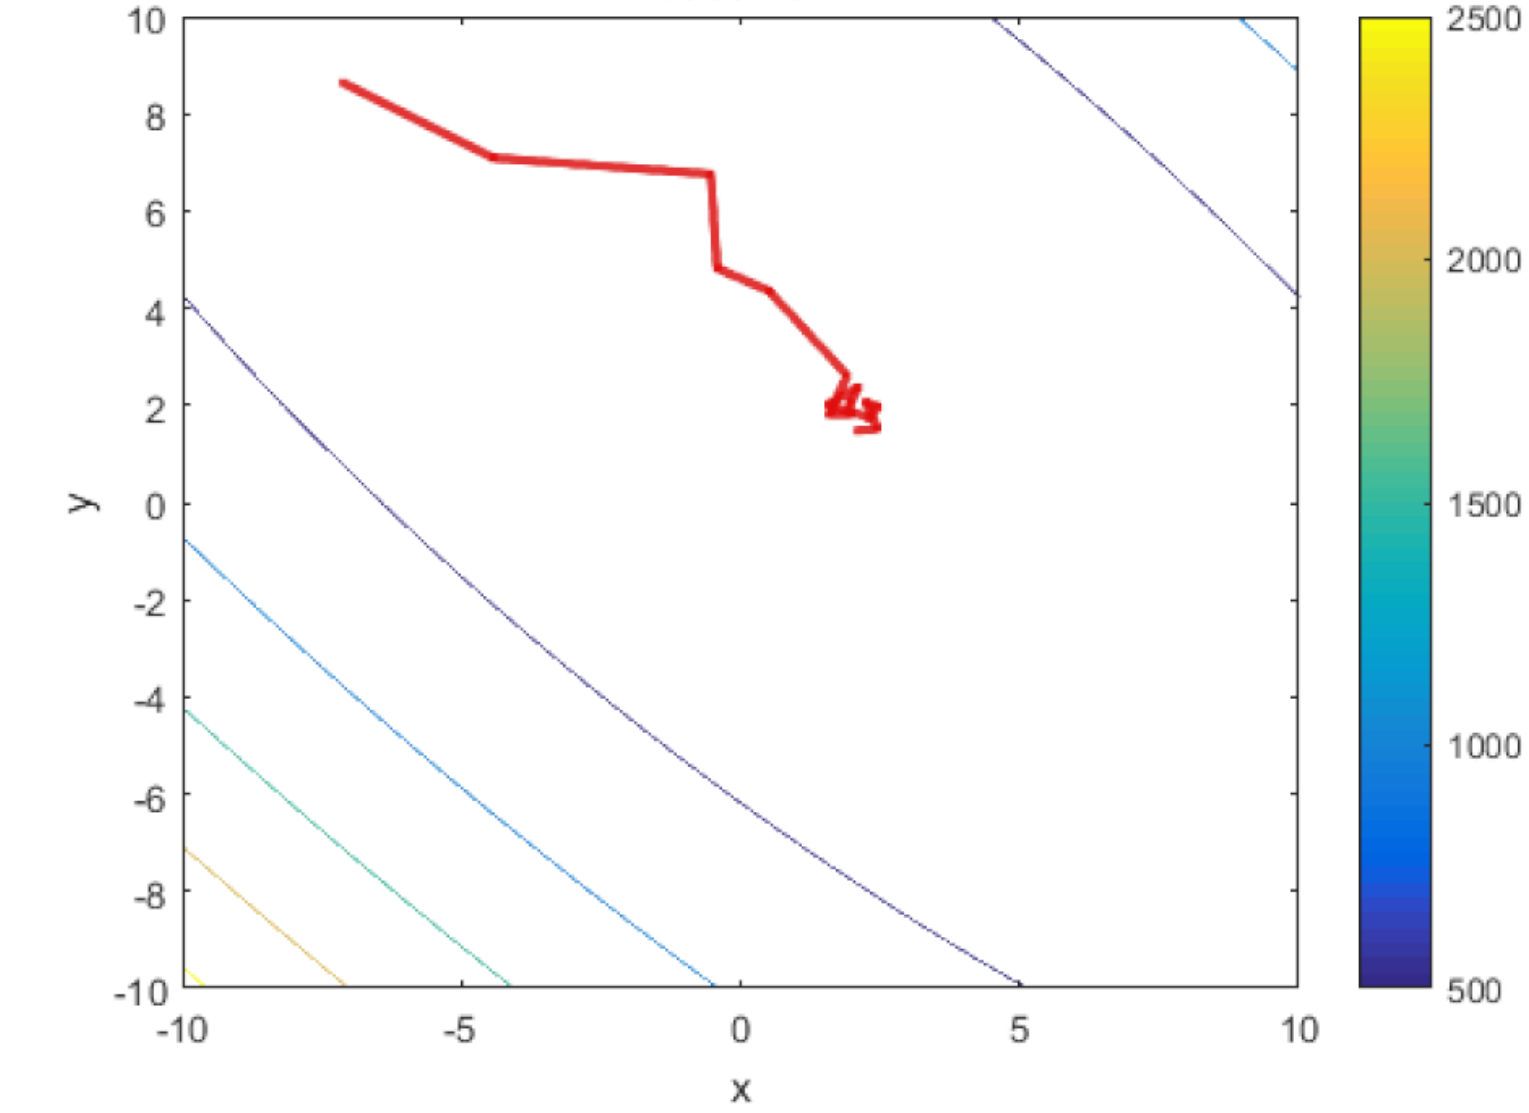
\includegraphics[width=.6\linewidth]{booth.png}
  \caption{Booth}
  \label{fig:figur:3}
\end{subfigure}%
\begin{subfigure}{.275\textwidth}
  \centering
  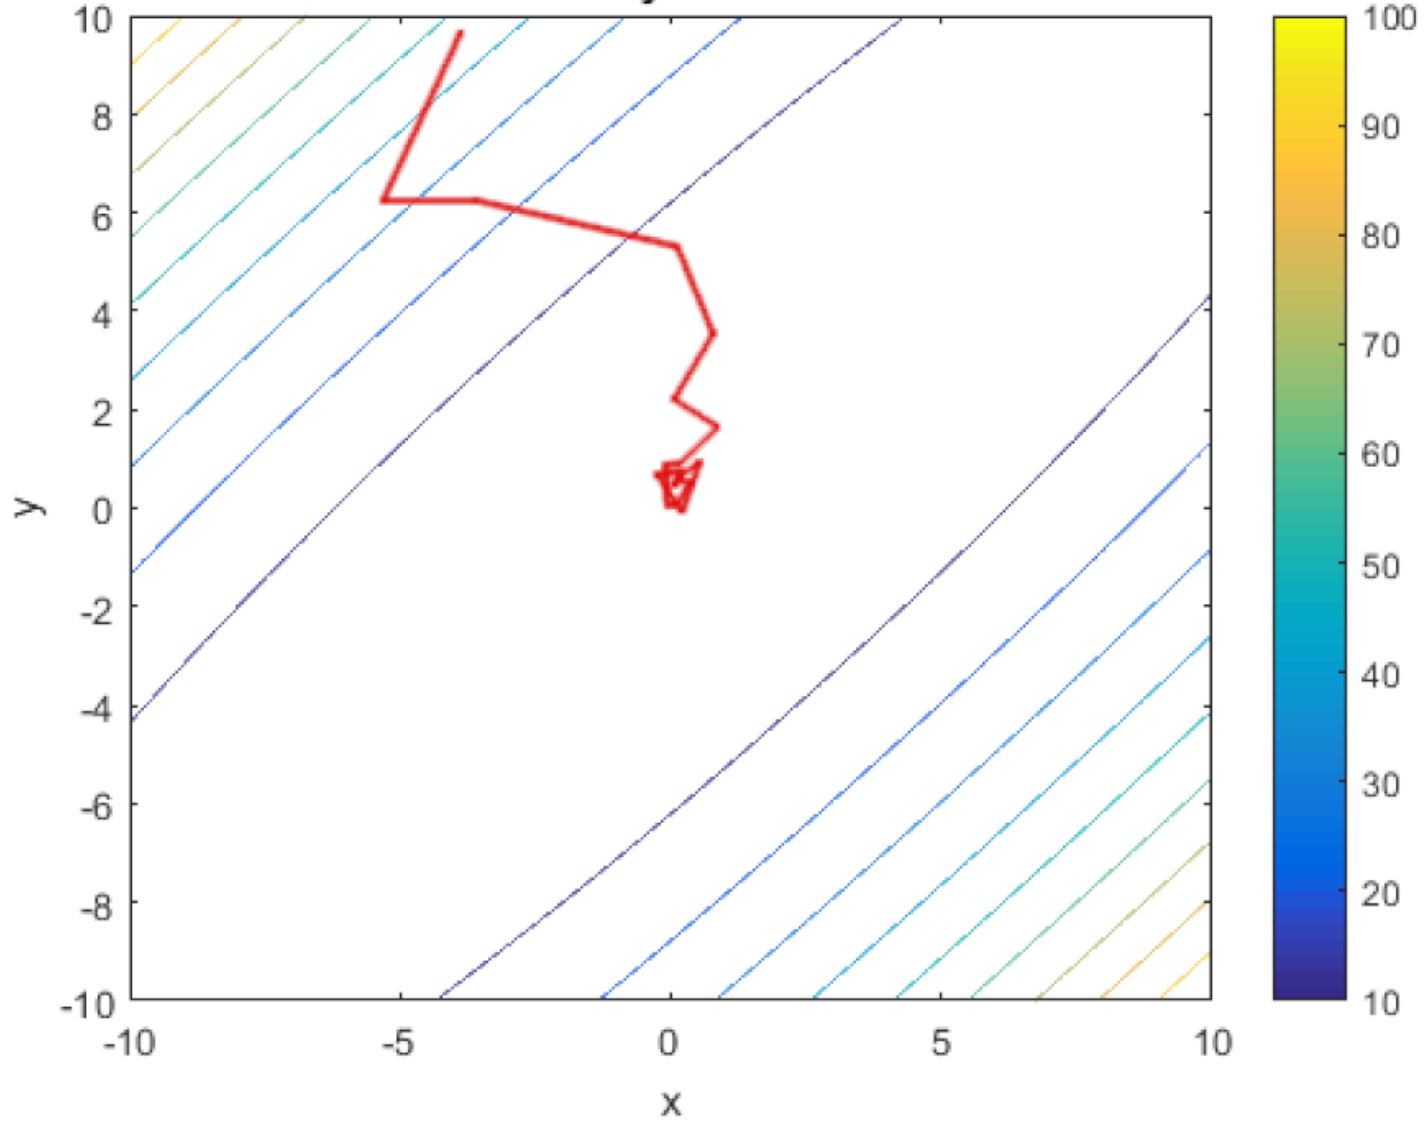
\includegraphics[width=.6\linewidth]{matyas.png}
  \caption{Matyas}
  \label{fig:figur:4}
\end{subfigure}
\begin{subfigure}{.275\textwidth}
  \centering
  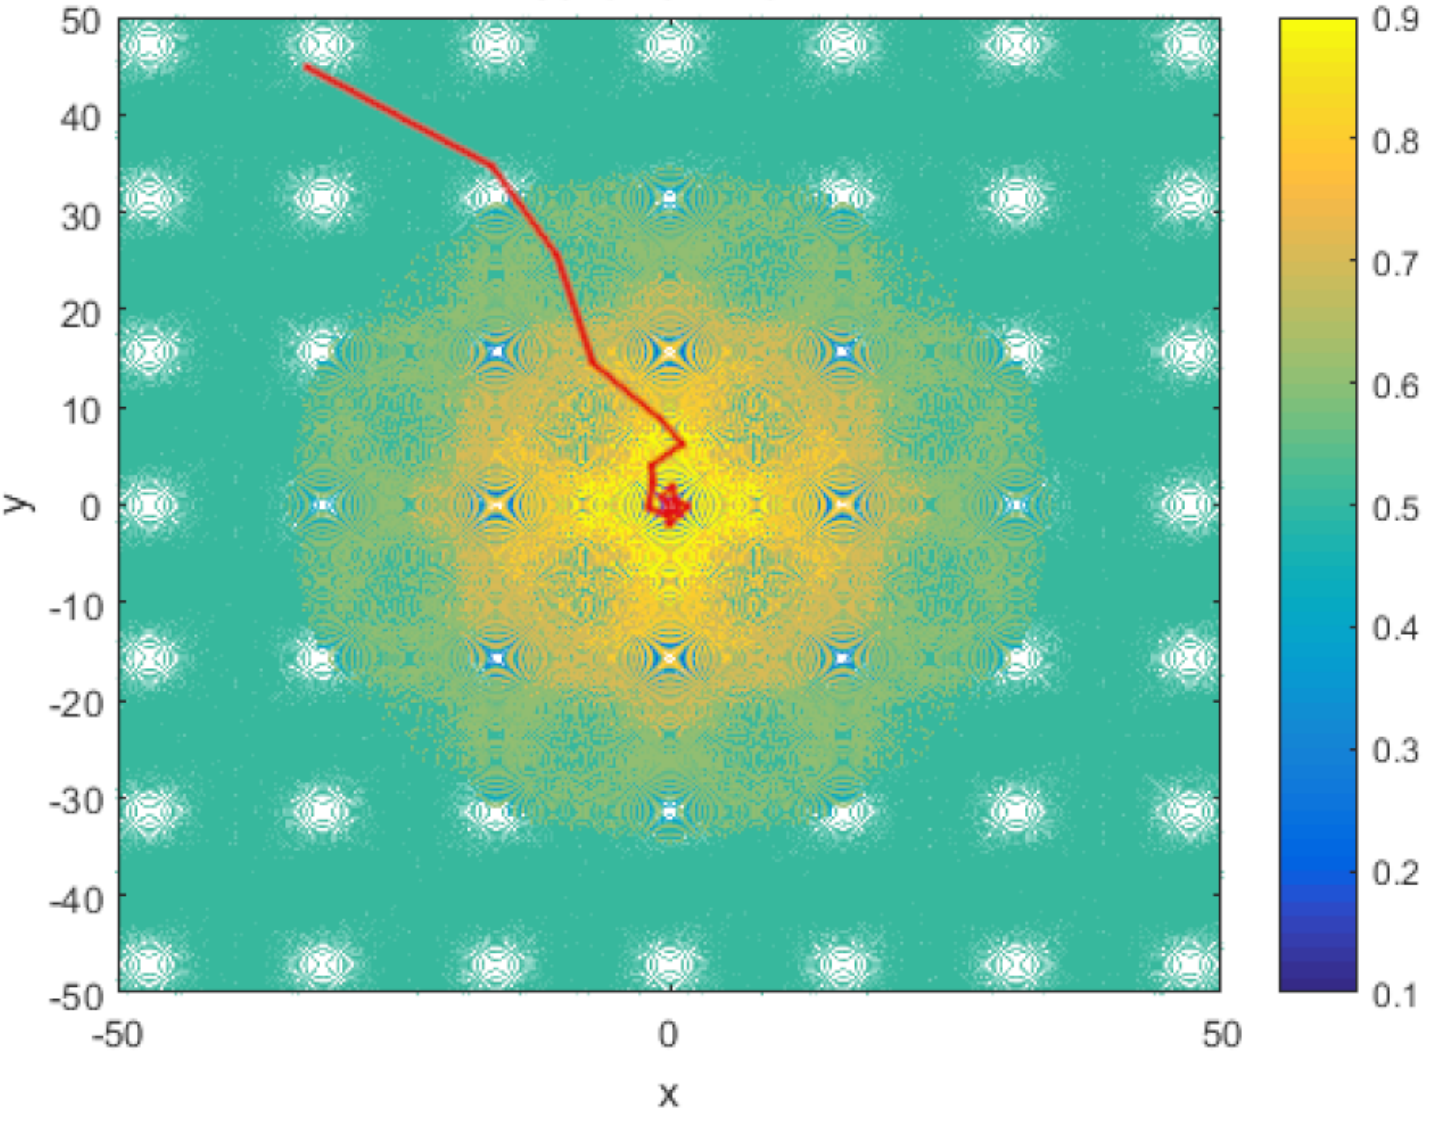
\includegraphics[width=.6\linewidth]{schaffern.png}
  \caption{Schaffern}
  \label{fig:figur:5}
\end{subfigure}%
\begin{subfigure}{.275\textwidth}
  \centering
  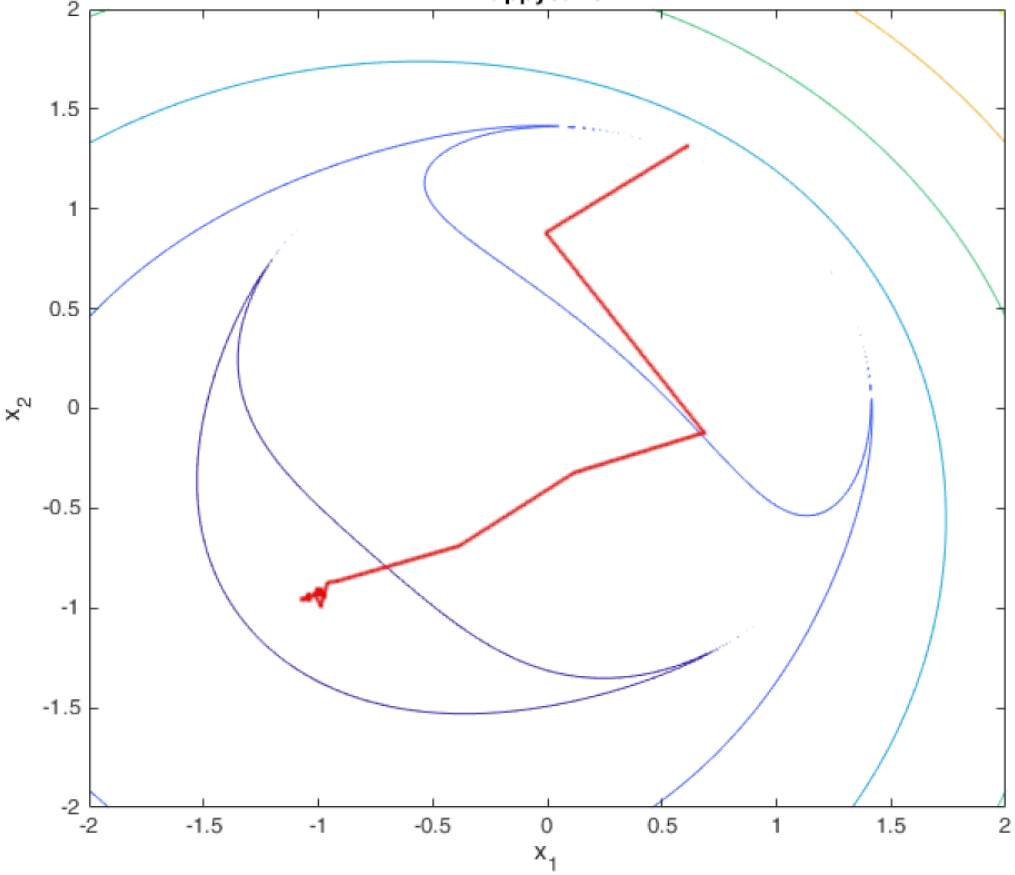
\includegraphics[width=.6\linewidth]{happycat.png}
  \caption{Happycat}
  \label{fig:figur:6}
\end{subfigure}
\caption{Departmant A Dominance}
% \label{fig:sfig6}
\end{figure}

% \begin{figure}[!t]
%   \centering
%   \label{figur}\caption{Department A Dominant}
% 
%   \subfloat[Ackley]{\label{figur:1}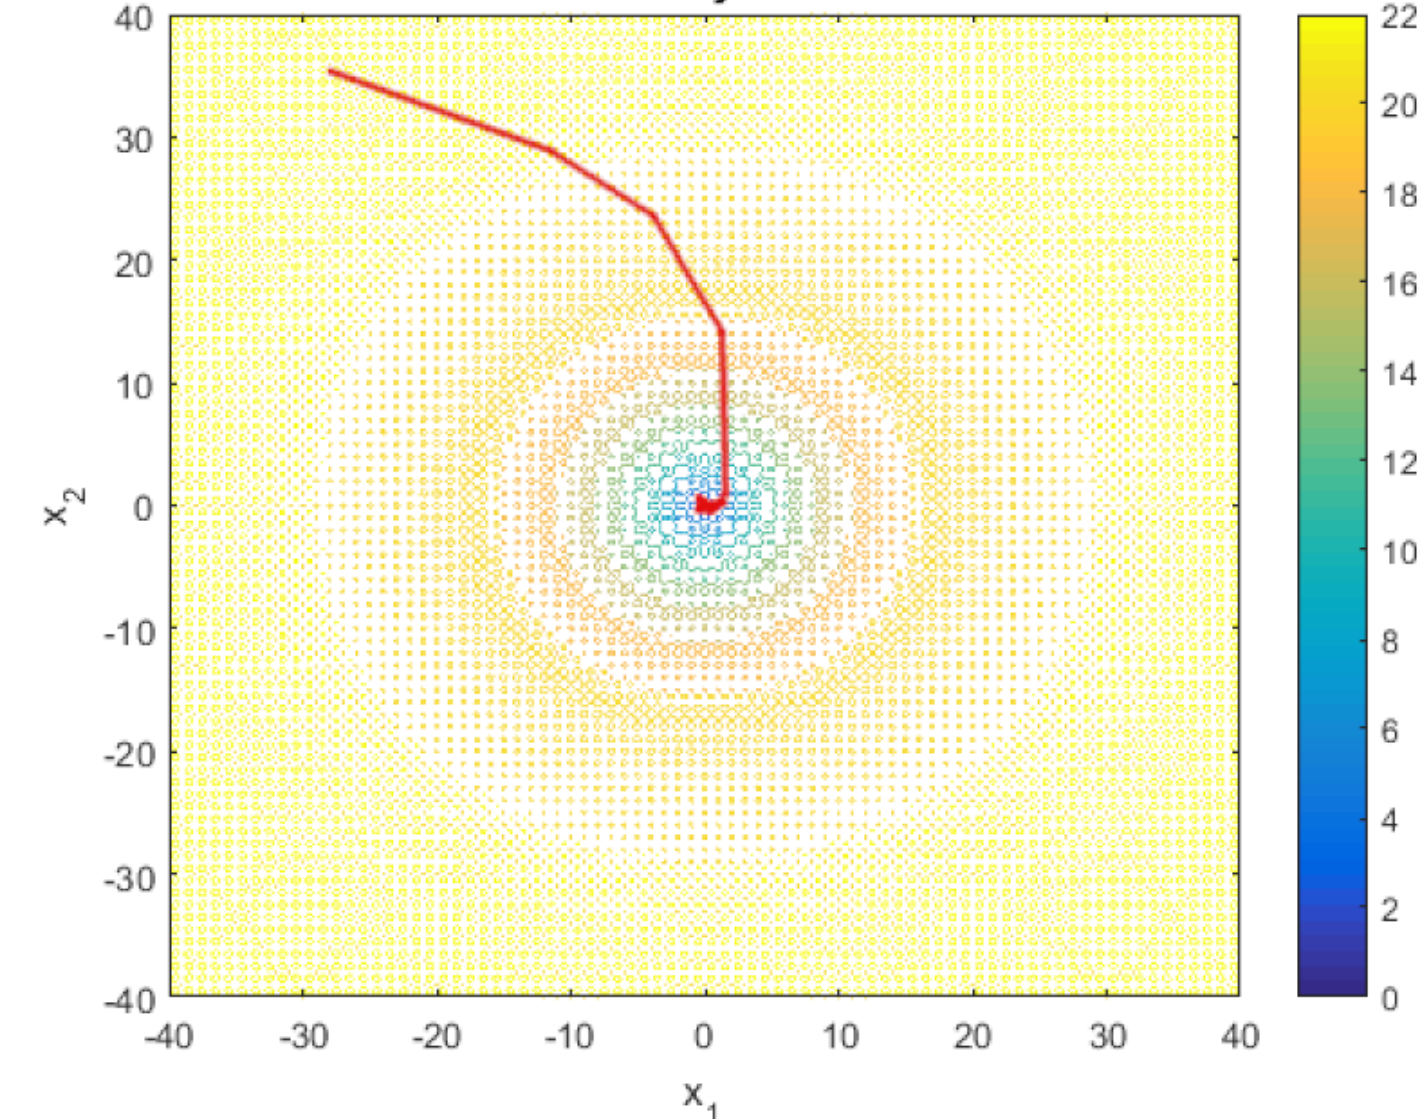
\includegraphics[width=50mm]{ackley.png}}
%   \subfloat[Bohachevskyn]{\label{figur:2}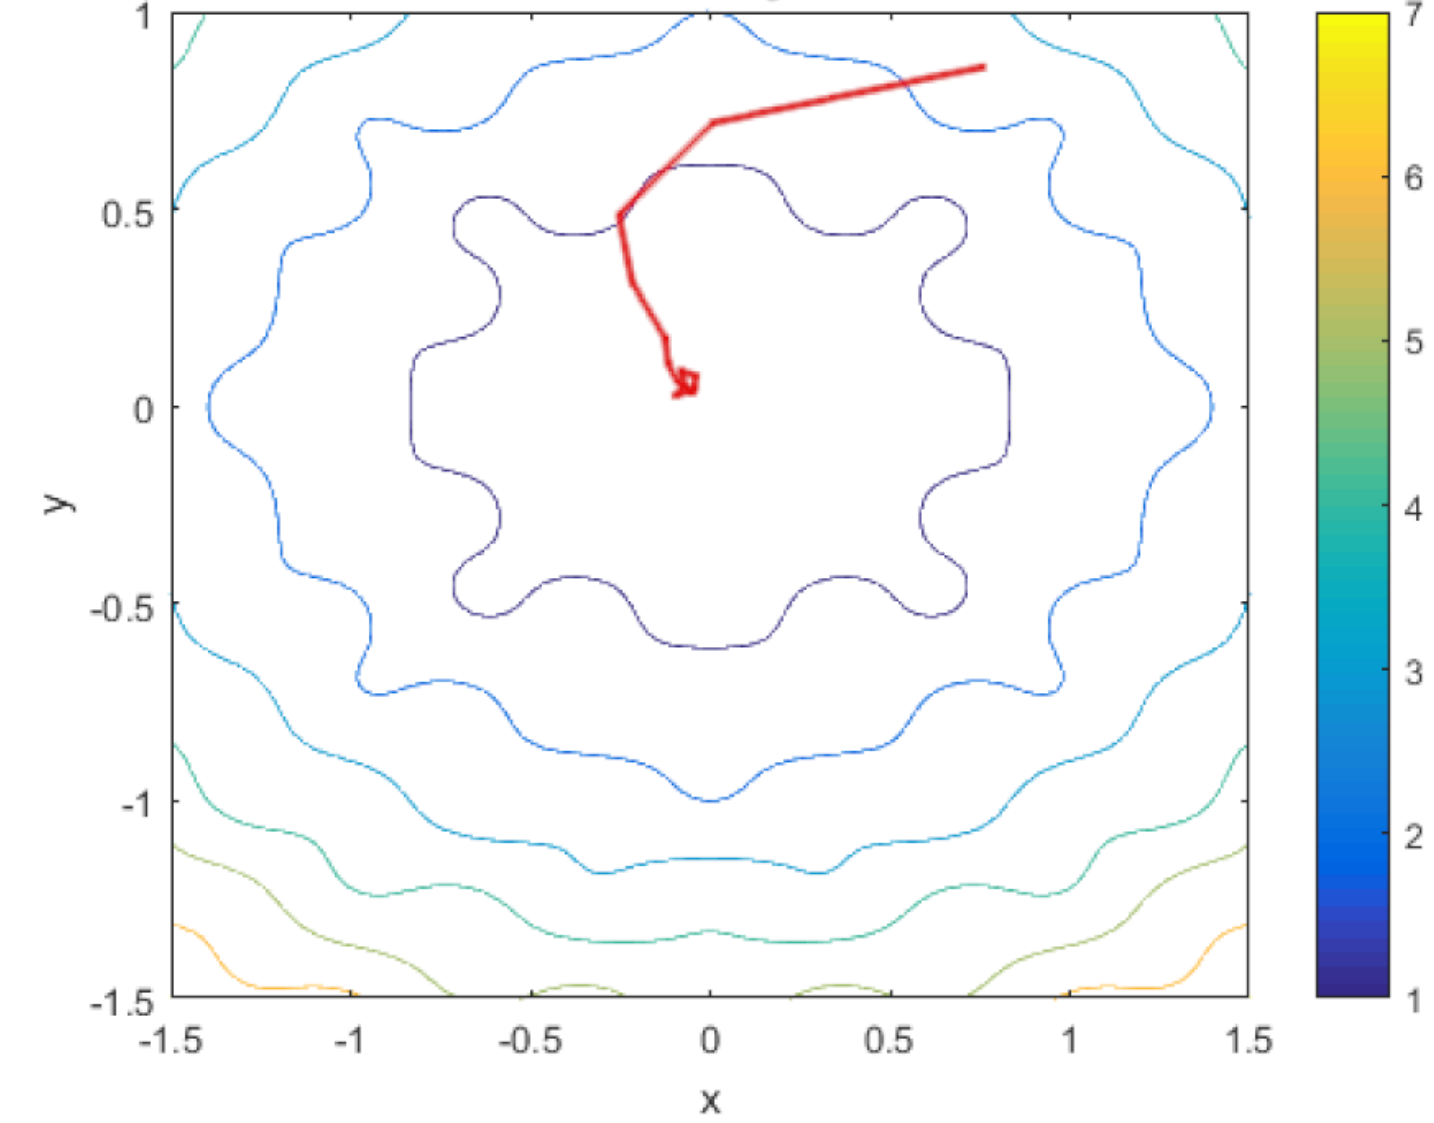
\includegraphics[width=50mm]{boha.png}}
%   \\
%   \subfloat[Booth]{\label{figur:3}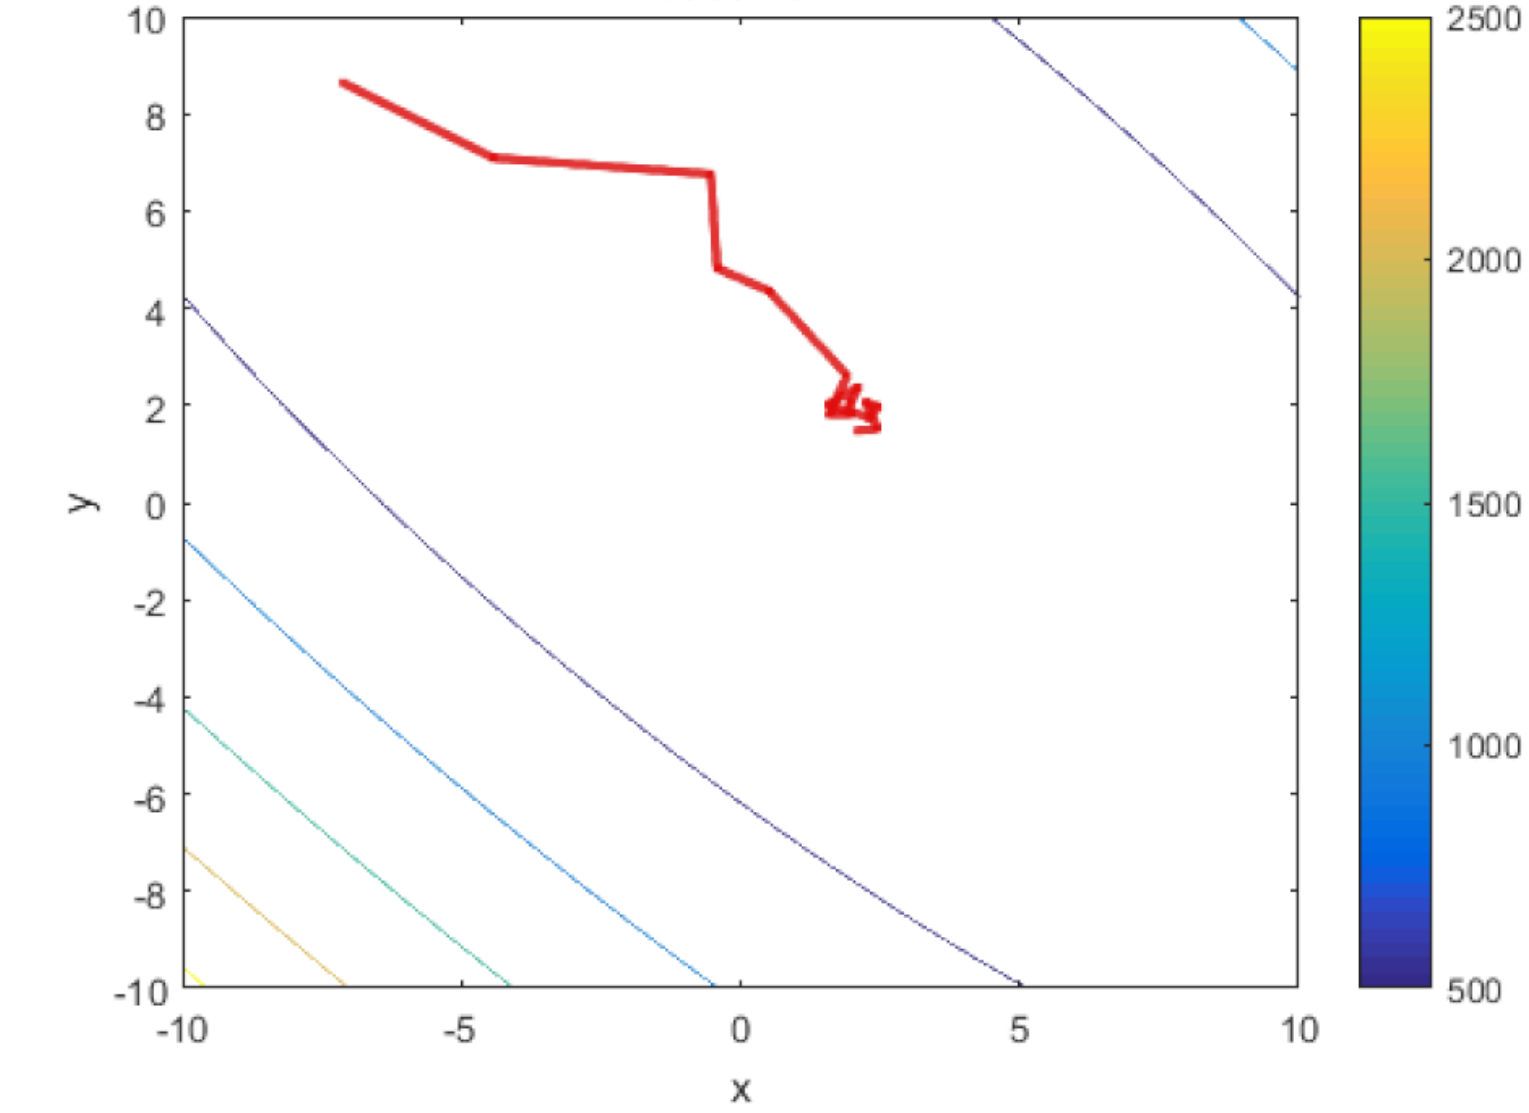
\includegraphics[width=50mm]{booth.png}}
%   \subfloat[Matyas]{\label{figur:4}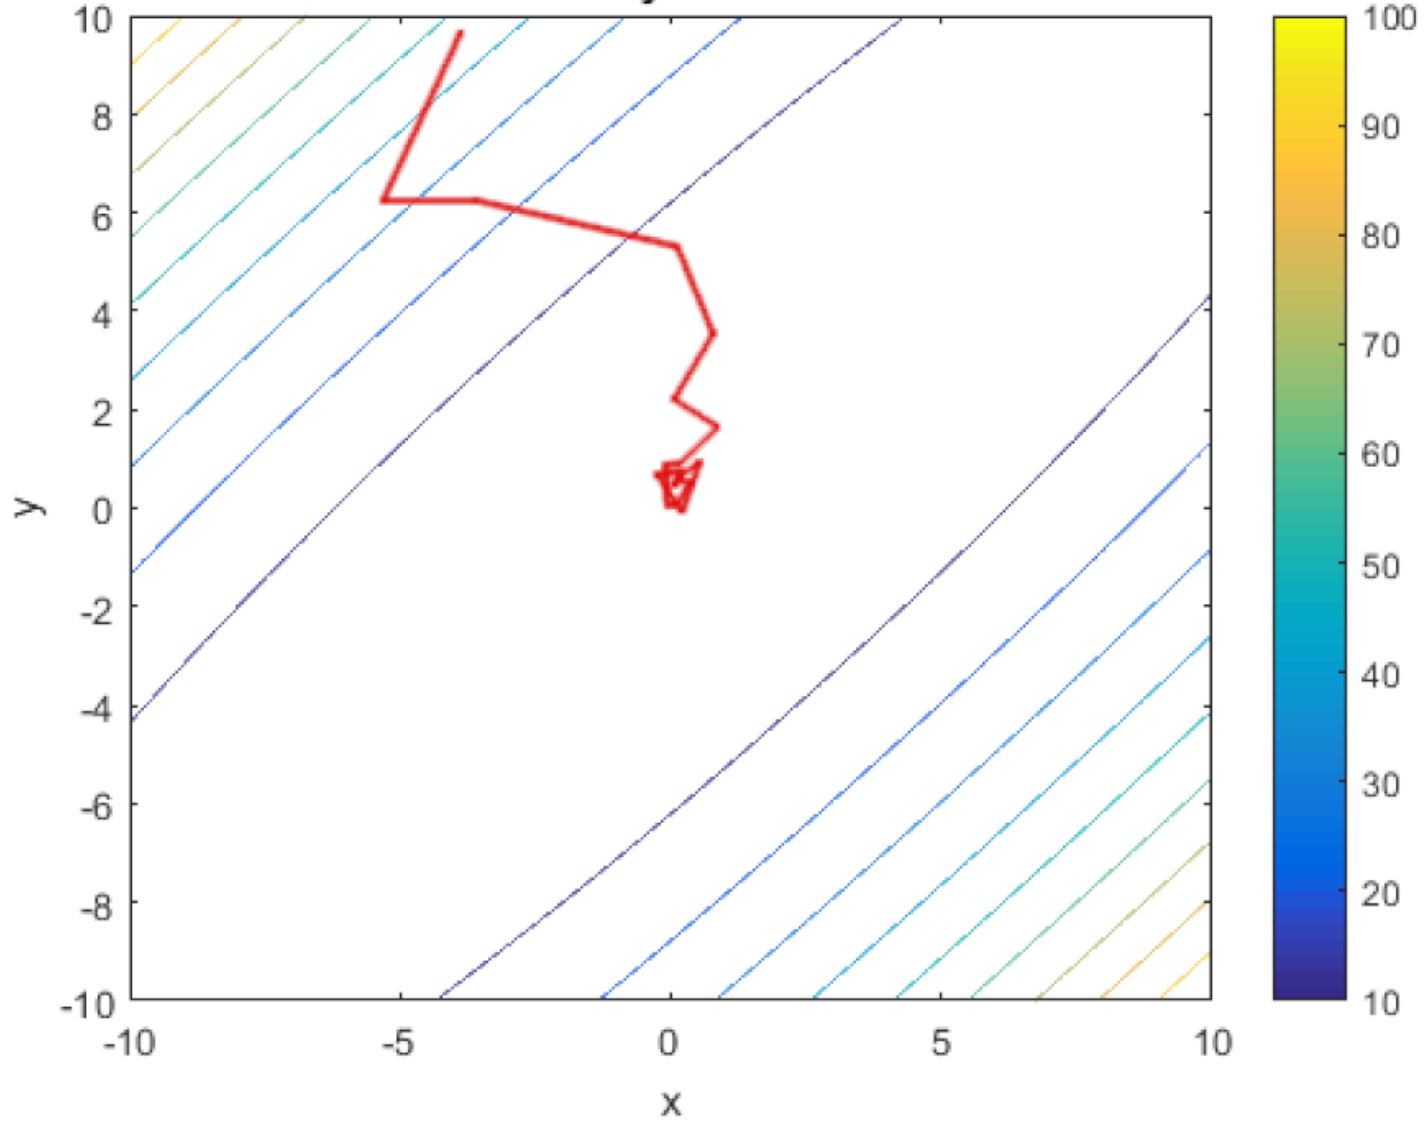
\includegraphics[width=50mm]{matyas.png}}
%   \\
%   \subfloat[Schaffern]{\label{figur:5}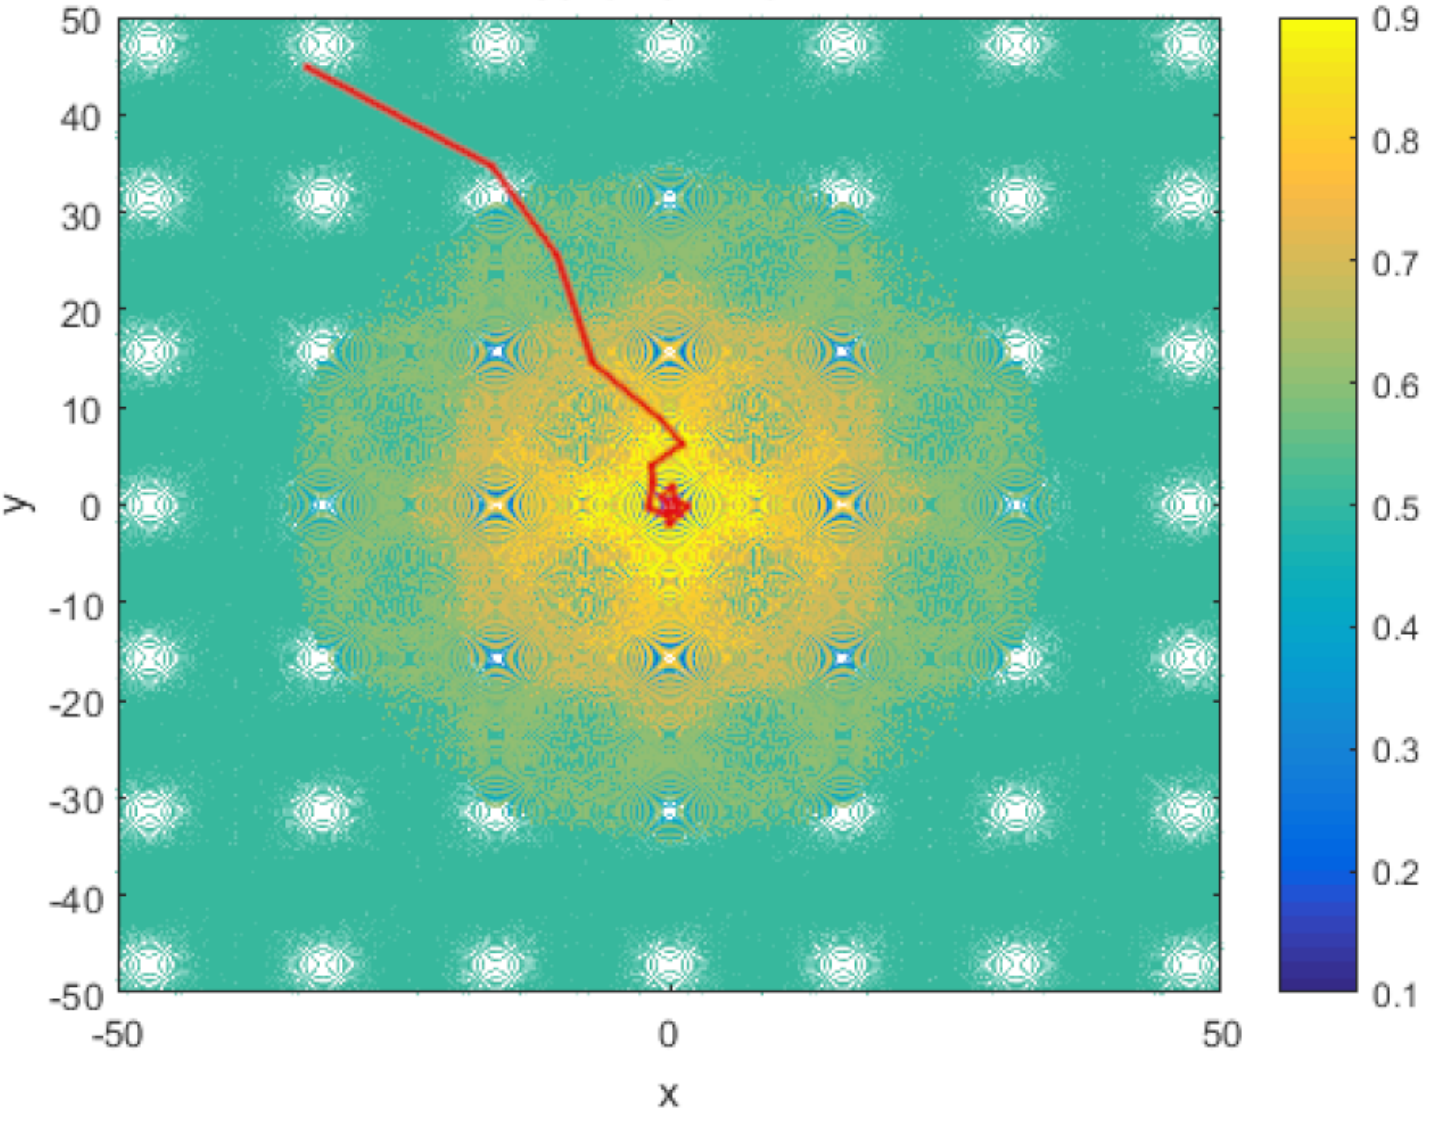
\includegraphics[width=50mm]{schaffern.png}}
%   \subfloat[Happy Cat]{\label{figur:6}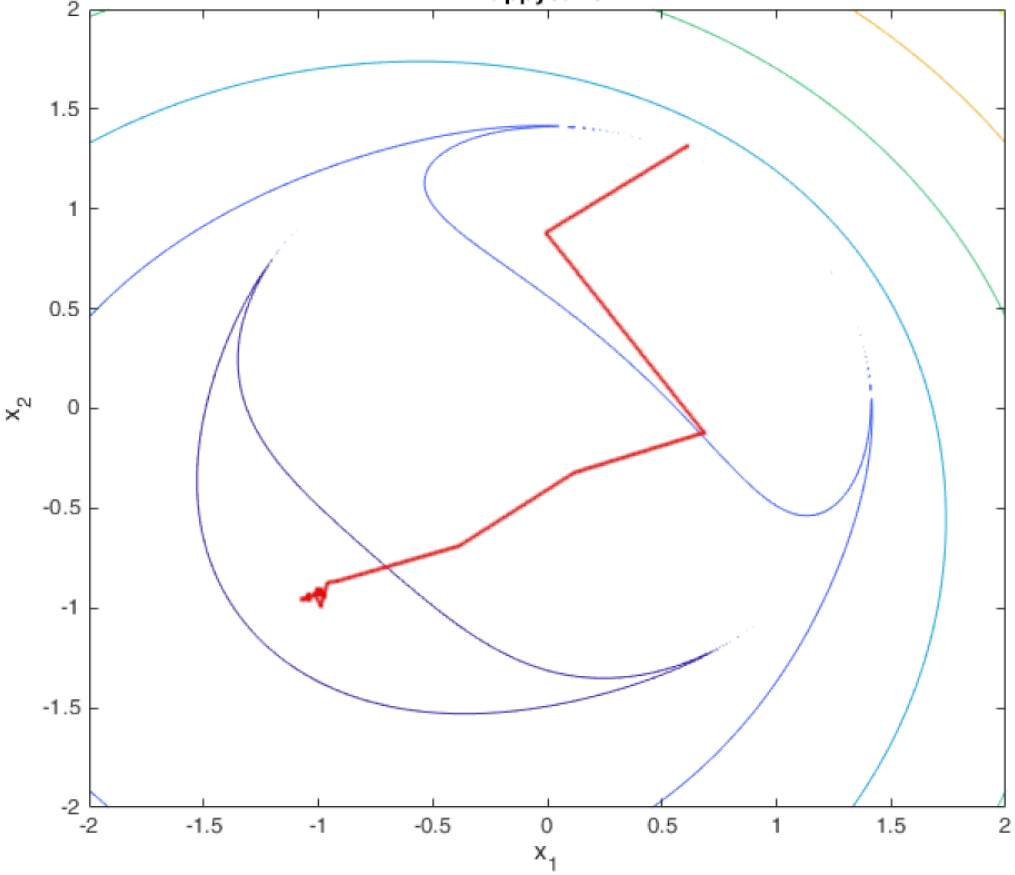
\includegraphics[width=43.5mm]{happycat.png}}
% \end{figure}

\begin{figure}[!t]
\begin{subfigure}{.275\textwidth}
  \centering
  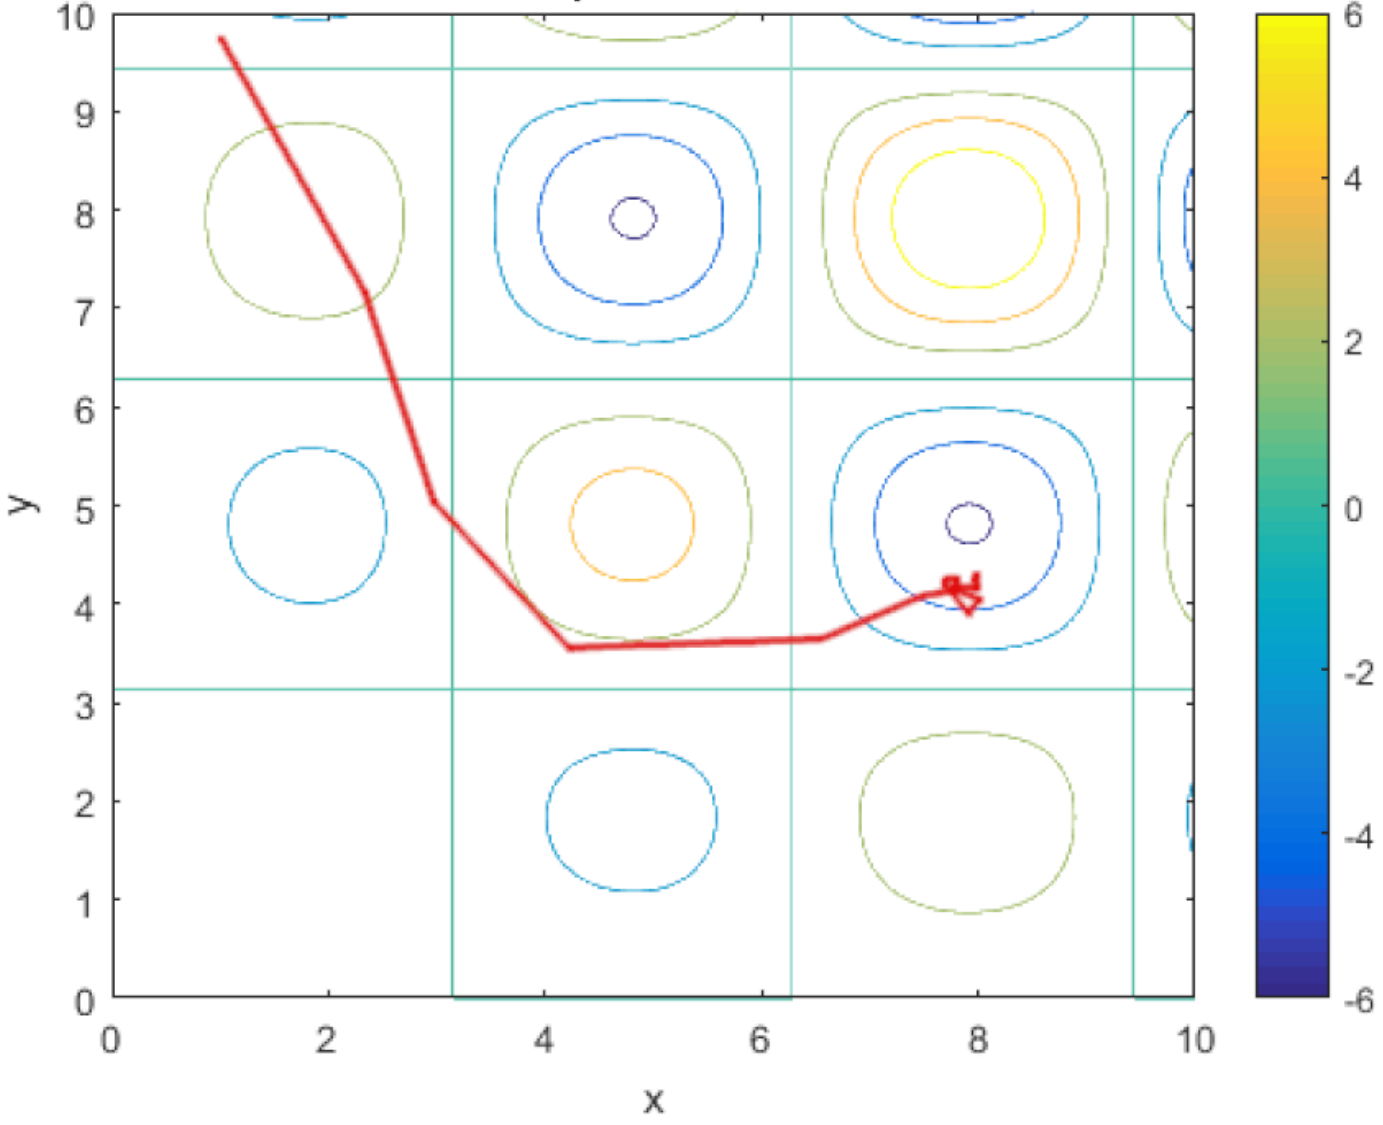
\includegraphics[width=.6\linewidth]{alpinea.png}
  \caption{Alpine-A}
  \label{fig:figur:7}
\end{subfigure}%
\begin{subfigure}{.275\textwidth}
  \centering
  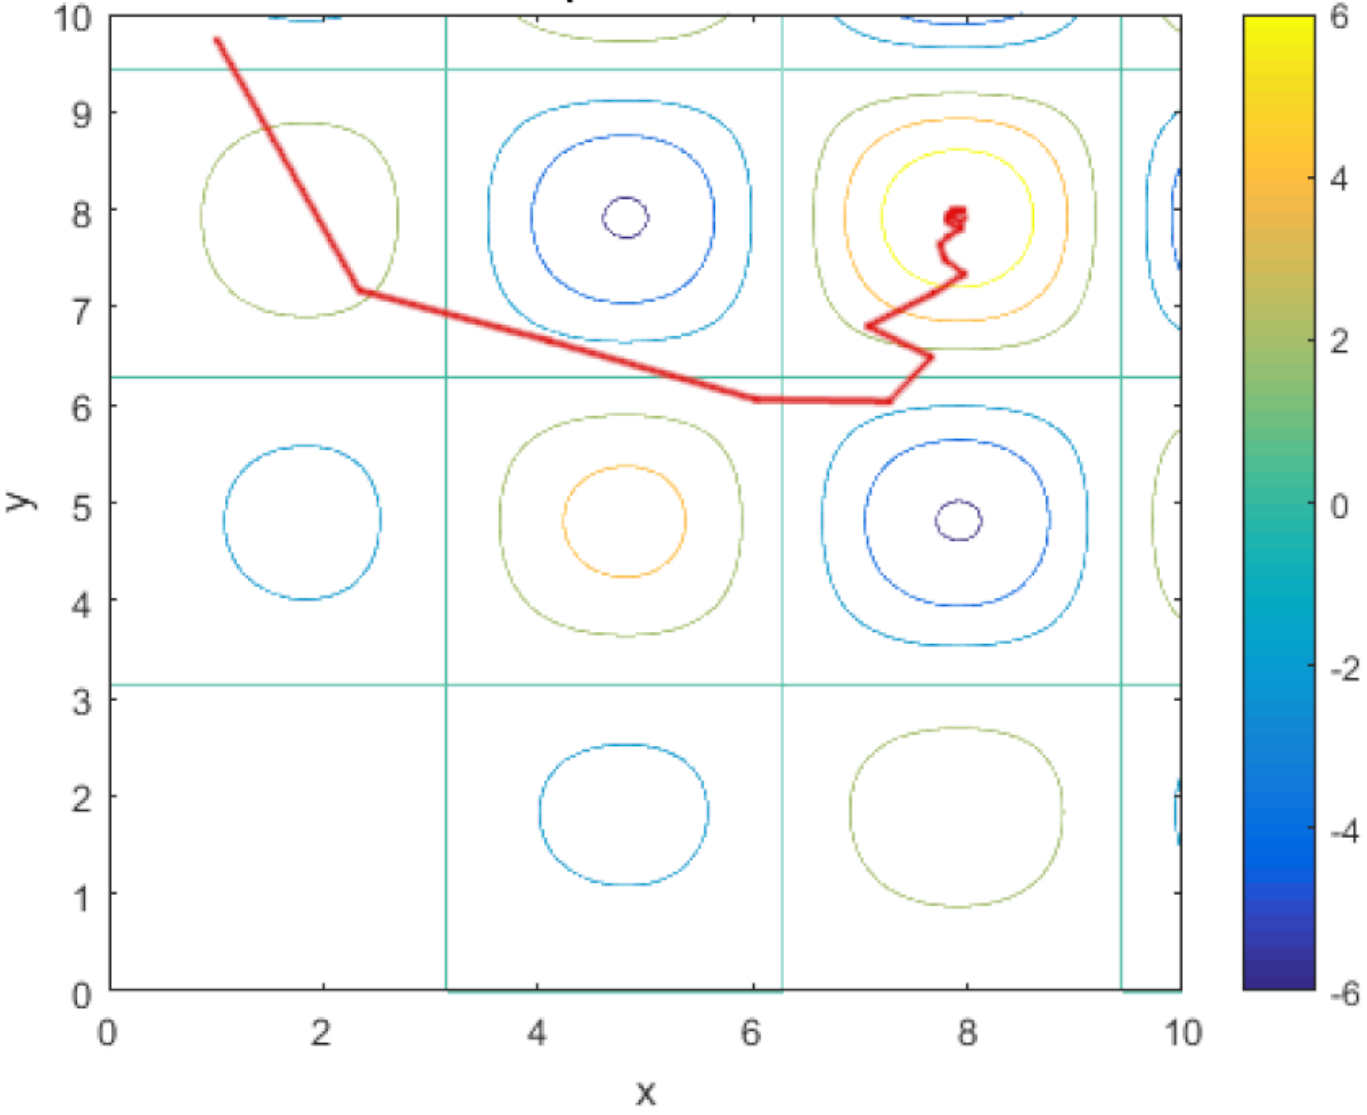
\includegraphics[width=.6\linewidth]{alpineb.png}
  \caption{Alpine-B}
  \label{fig:figur:8}
\end{subfigure}
\begin{subfigure}{.275\textwidth}
  \centering
  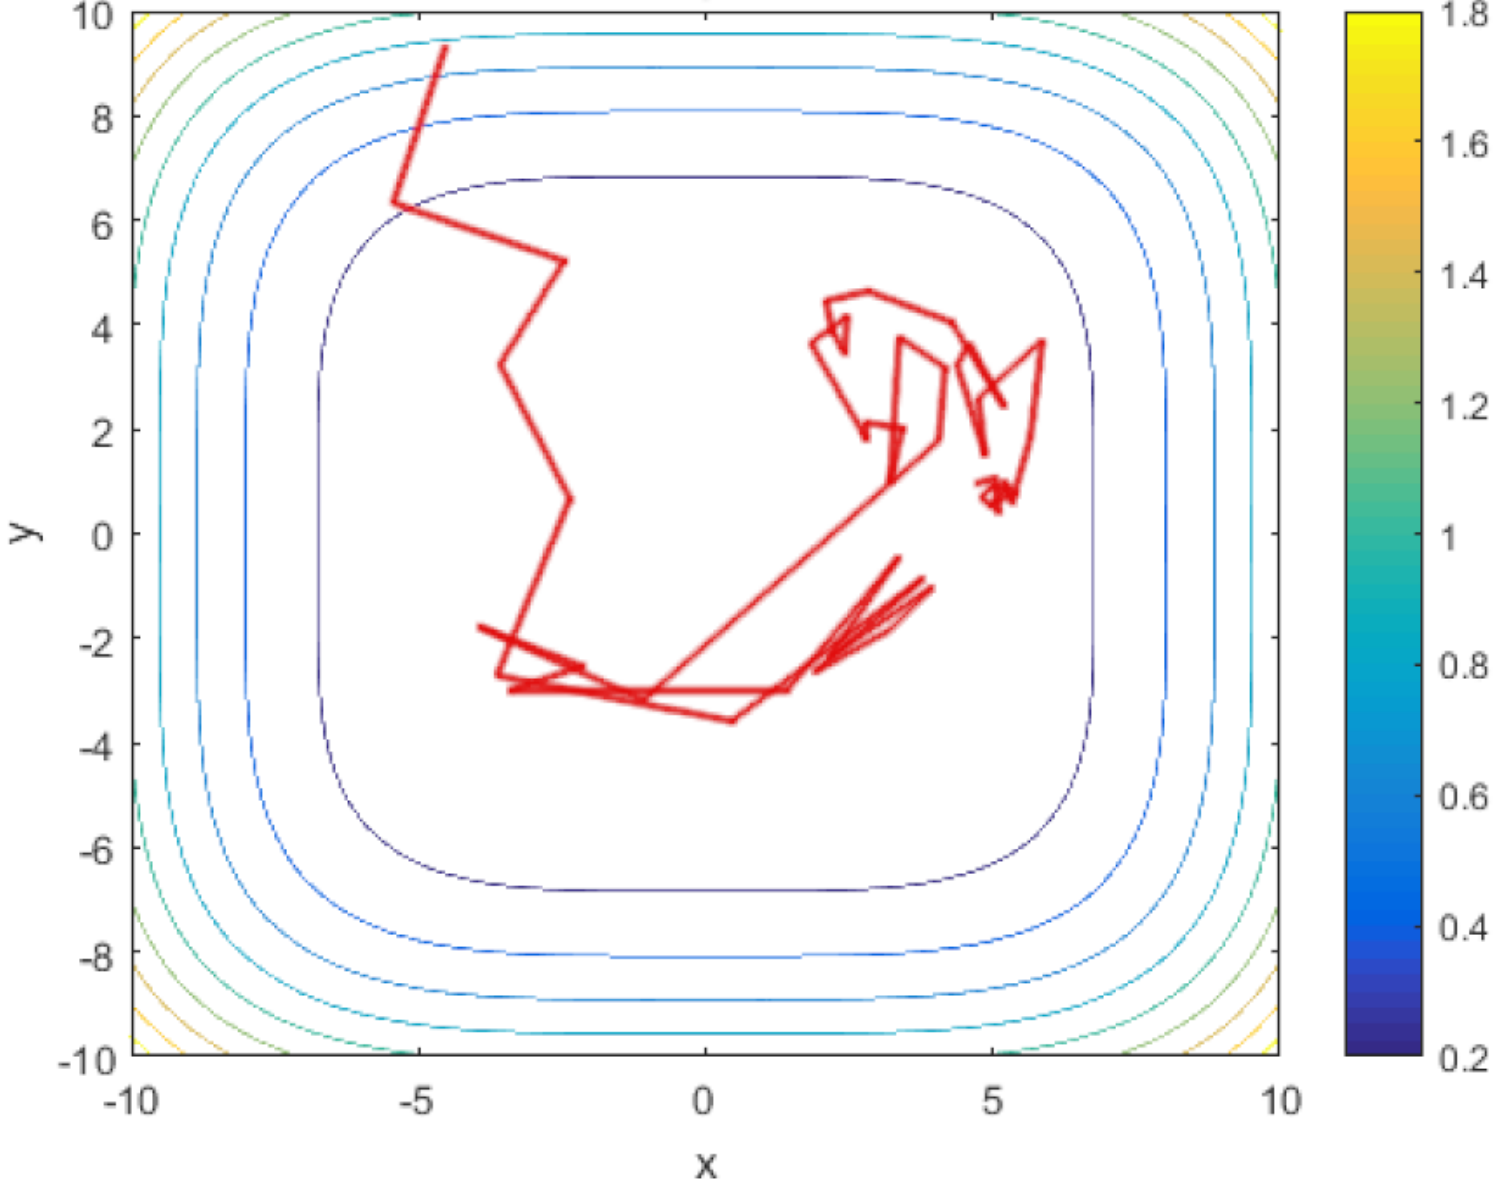
\includegraphics[width=.6\linewidth]{qinga.png}
  \caption{Qing-A}
  \label{fig:figur:9}
\end{subfigure}%
\begin{subfigure}{.275\textwidth}
  \centering
  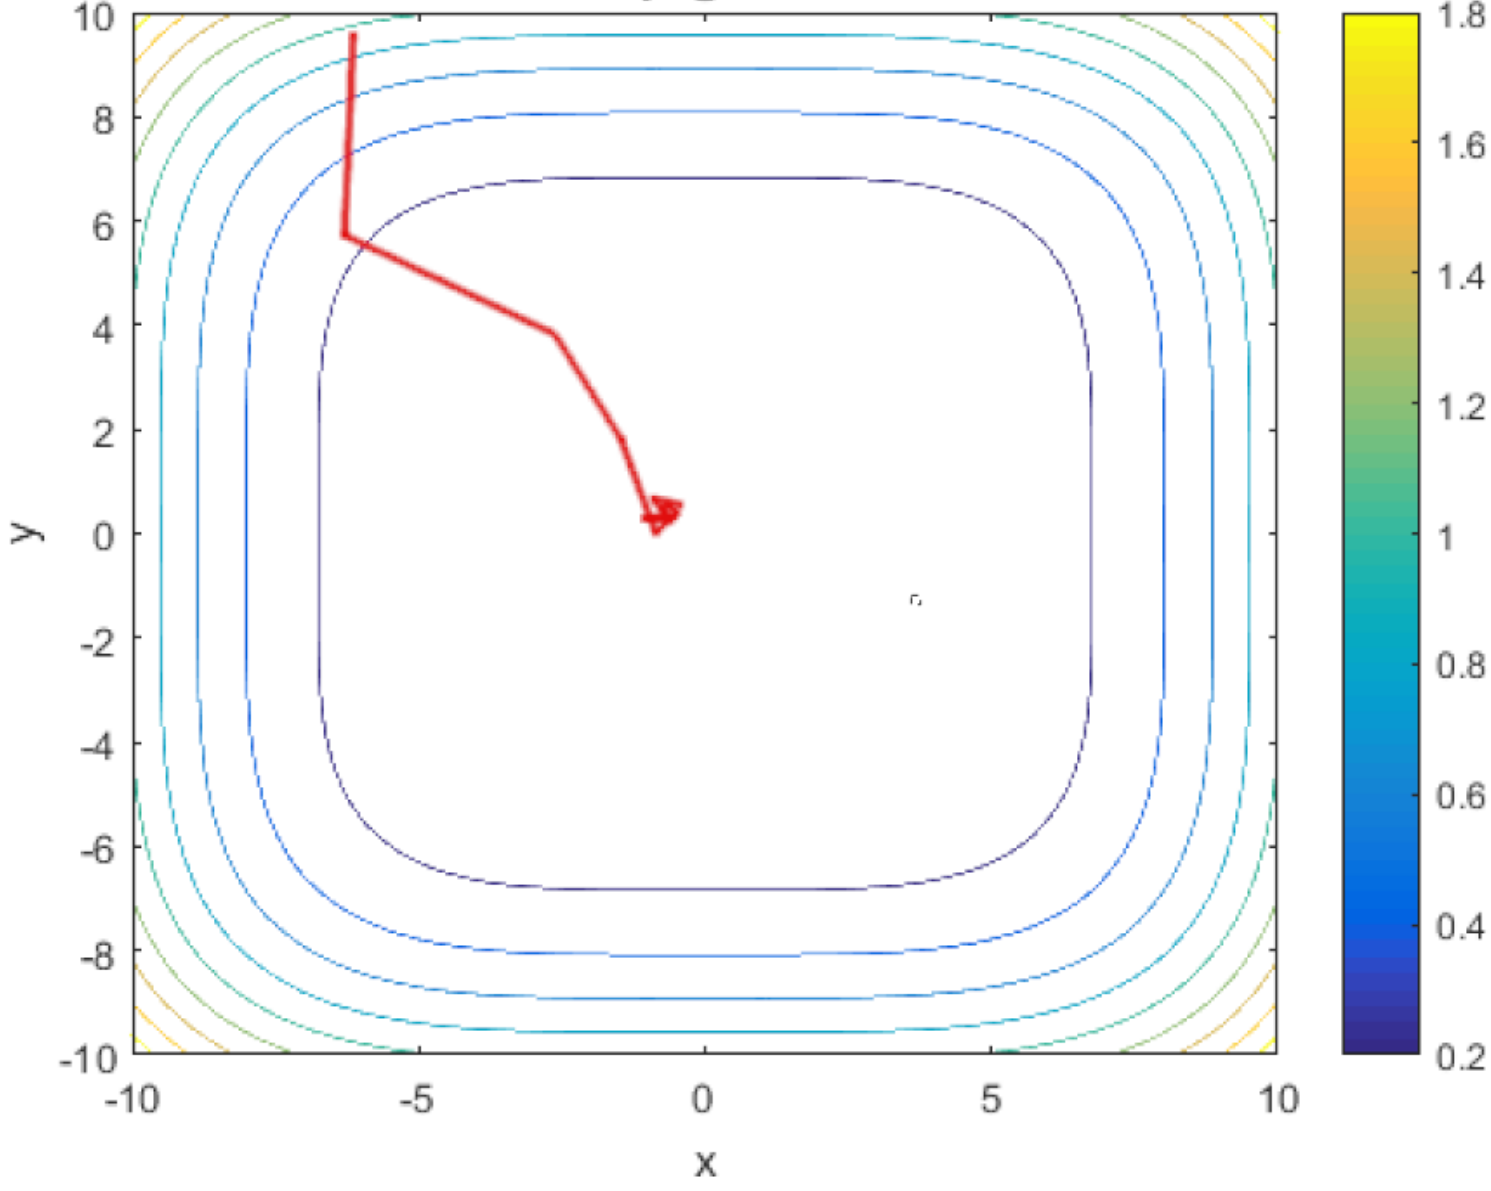
\includegraphics[width=.6\linewidth]{qingb.png}
  \caption{Qing-B}
  \label{fig:figur:10}
\end{subfigure}
\begin{subfigure}{.275\textwidth}
  \centering
  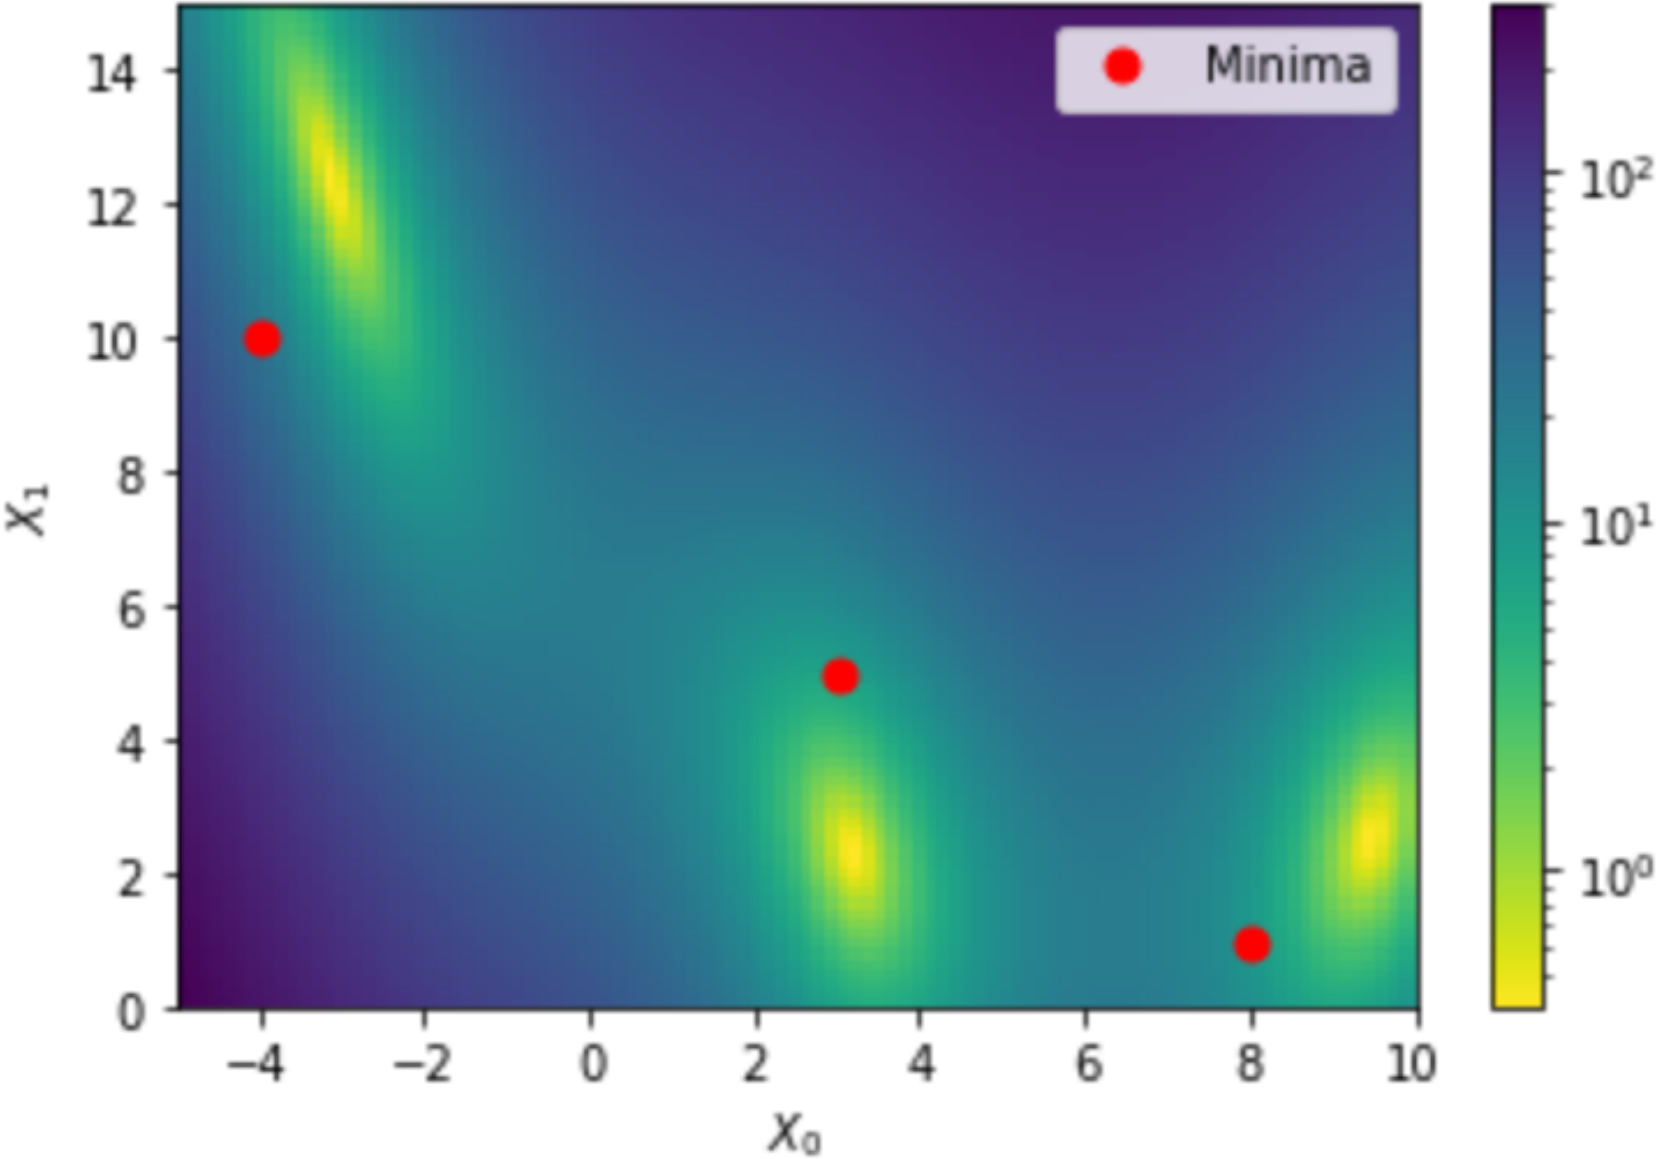
\includegraphics[width=.6\linewidth]{branina.png}
  \caption{Branin-A}
  \label{fig:figur:11}
\end{subfigure}%
\begin{subfigure}{.275\textwidth}
  \centering
  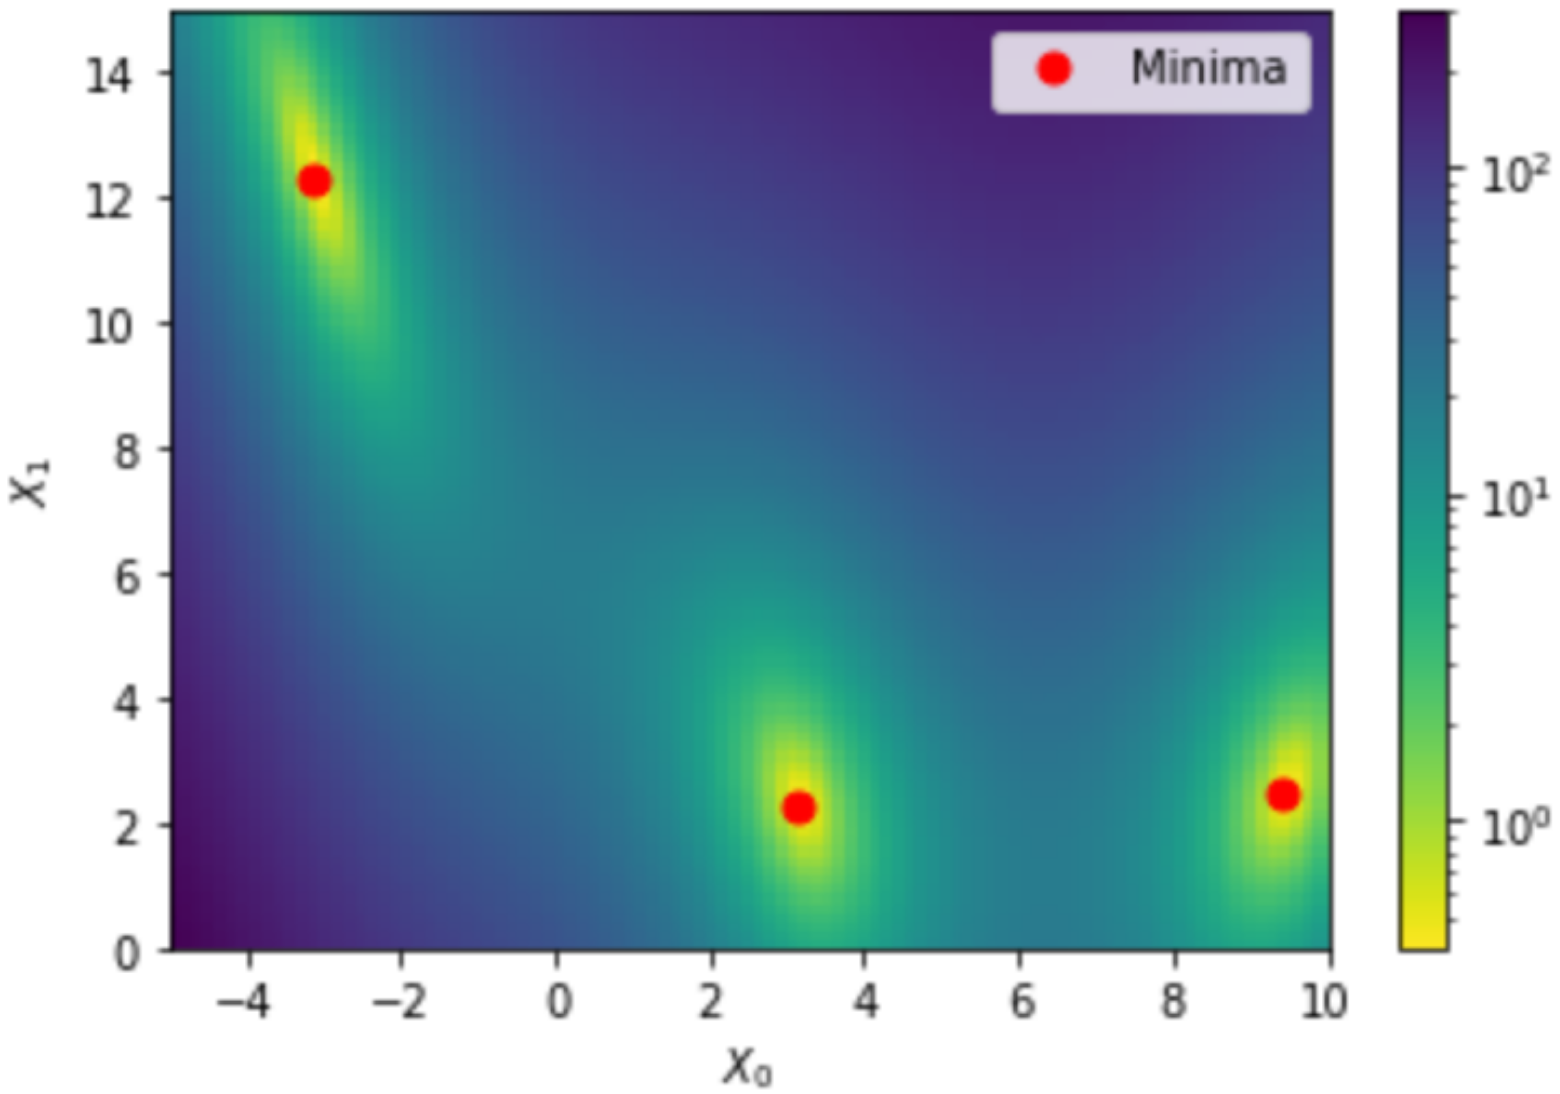
\includegraphics[width=.6\linewidth]{braninb.png}
  \caption{Branin-B}
  \label{fig:figur:12}
\end{subfigure}
\caption{Departmant B Dominance}
% \label{fig:sfig6}
\end{figure}

% \begin{figure}[!t]
%   \centering
%   \label{figur}\caption{Department B Dominant}
% 
%   \subfloat[Alpine-A]{\label{figur:7}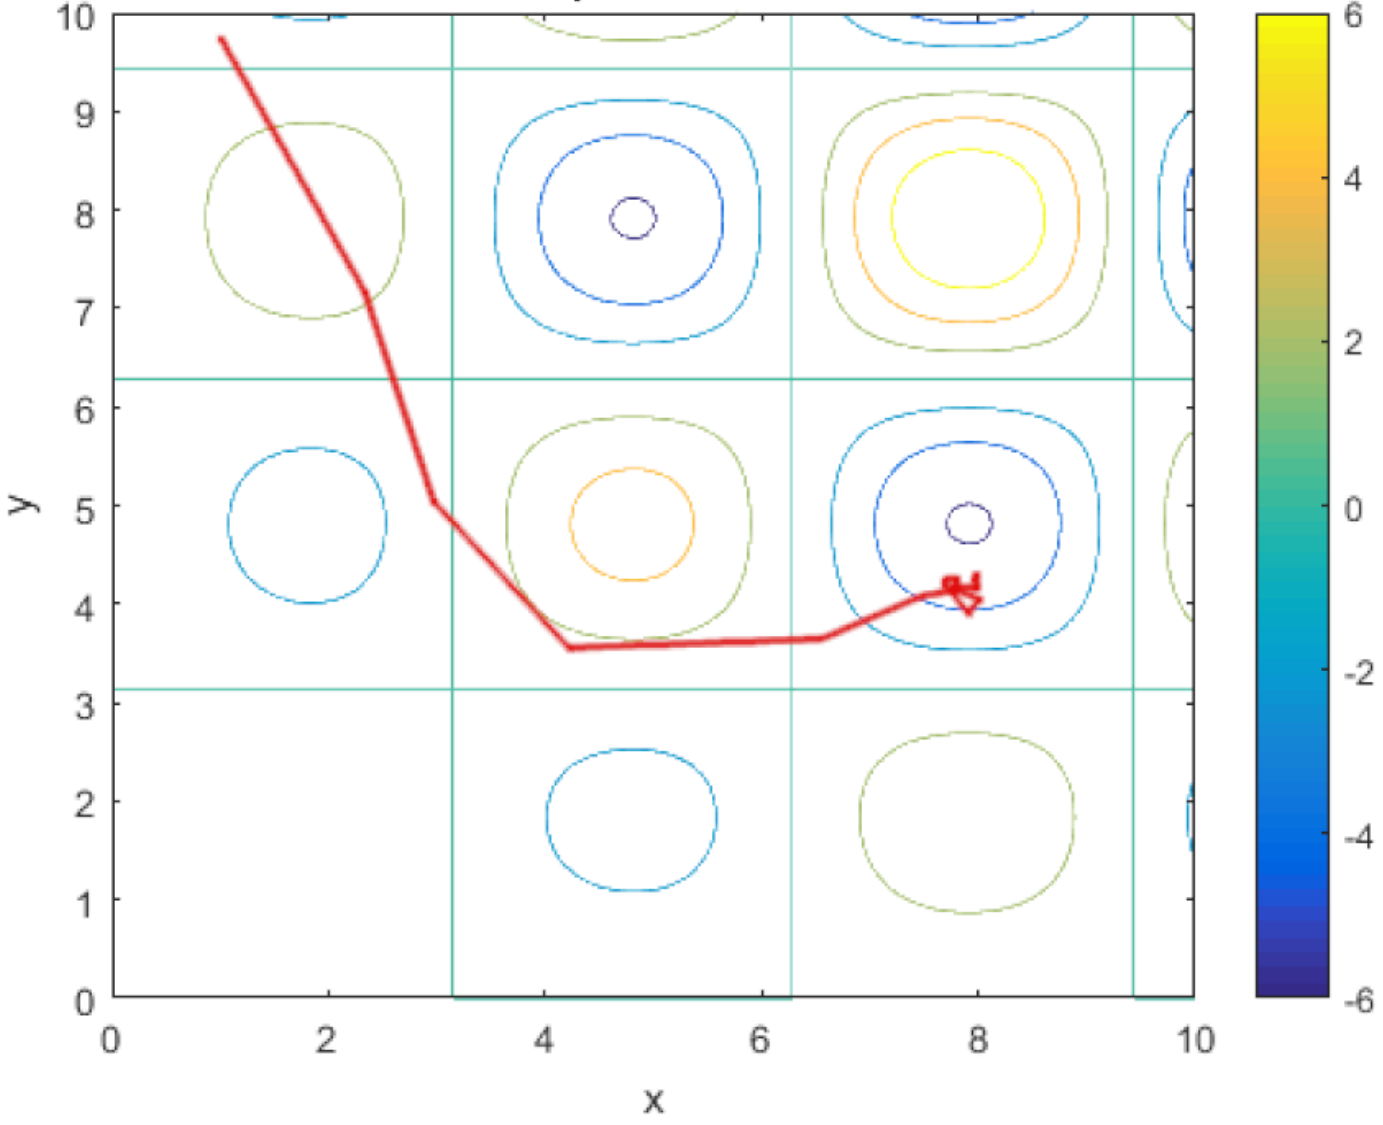
\includegraphics[width=45mm]{alpinea.png}}
%   \subfloat[Alpine-B]{\label{figur:8}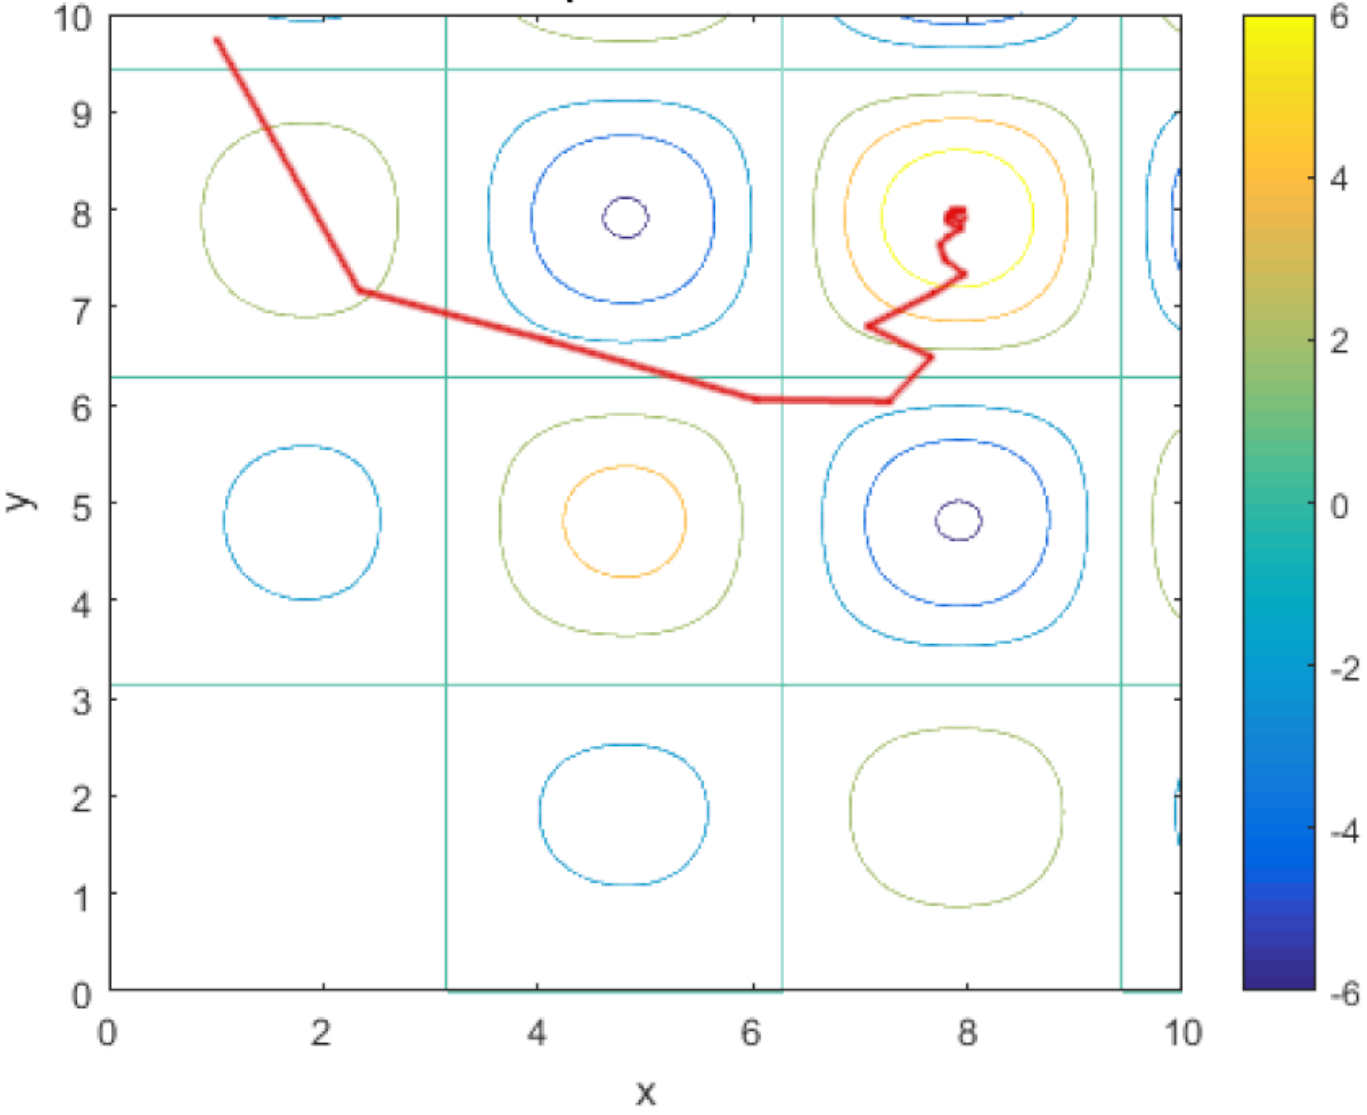
\includegraphics[width=45mm]{alpineb.png}}
%   \\
%   \subfloat[Qing-A]{\label{figur:9}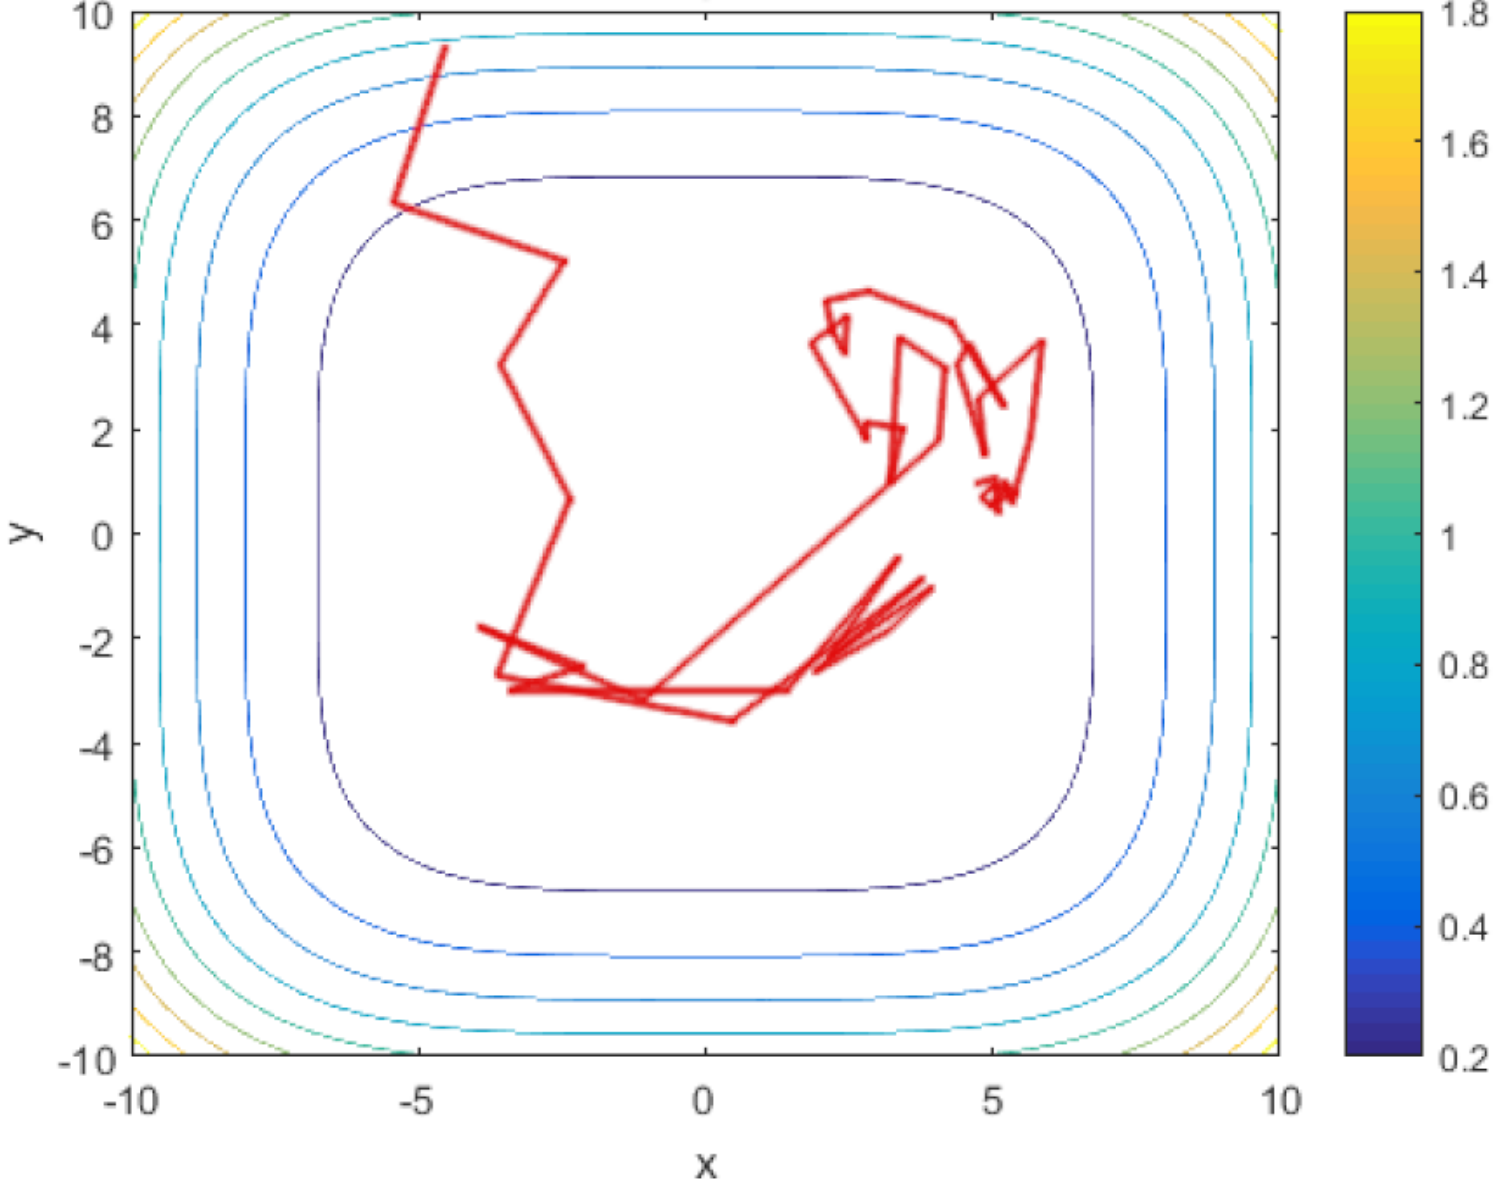
\includegraphics[width=37mm]{qinga.png}}
%   \subfloat[Qing-B]{\label{figur:10}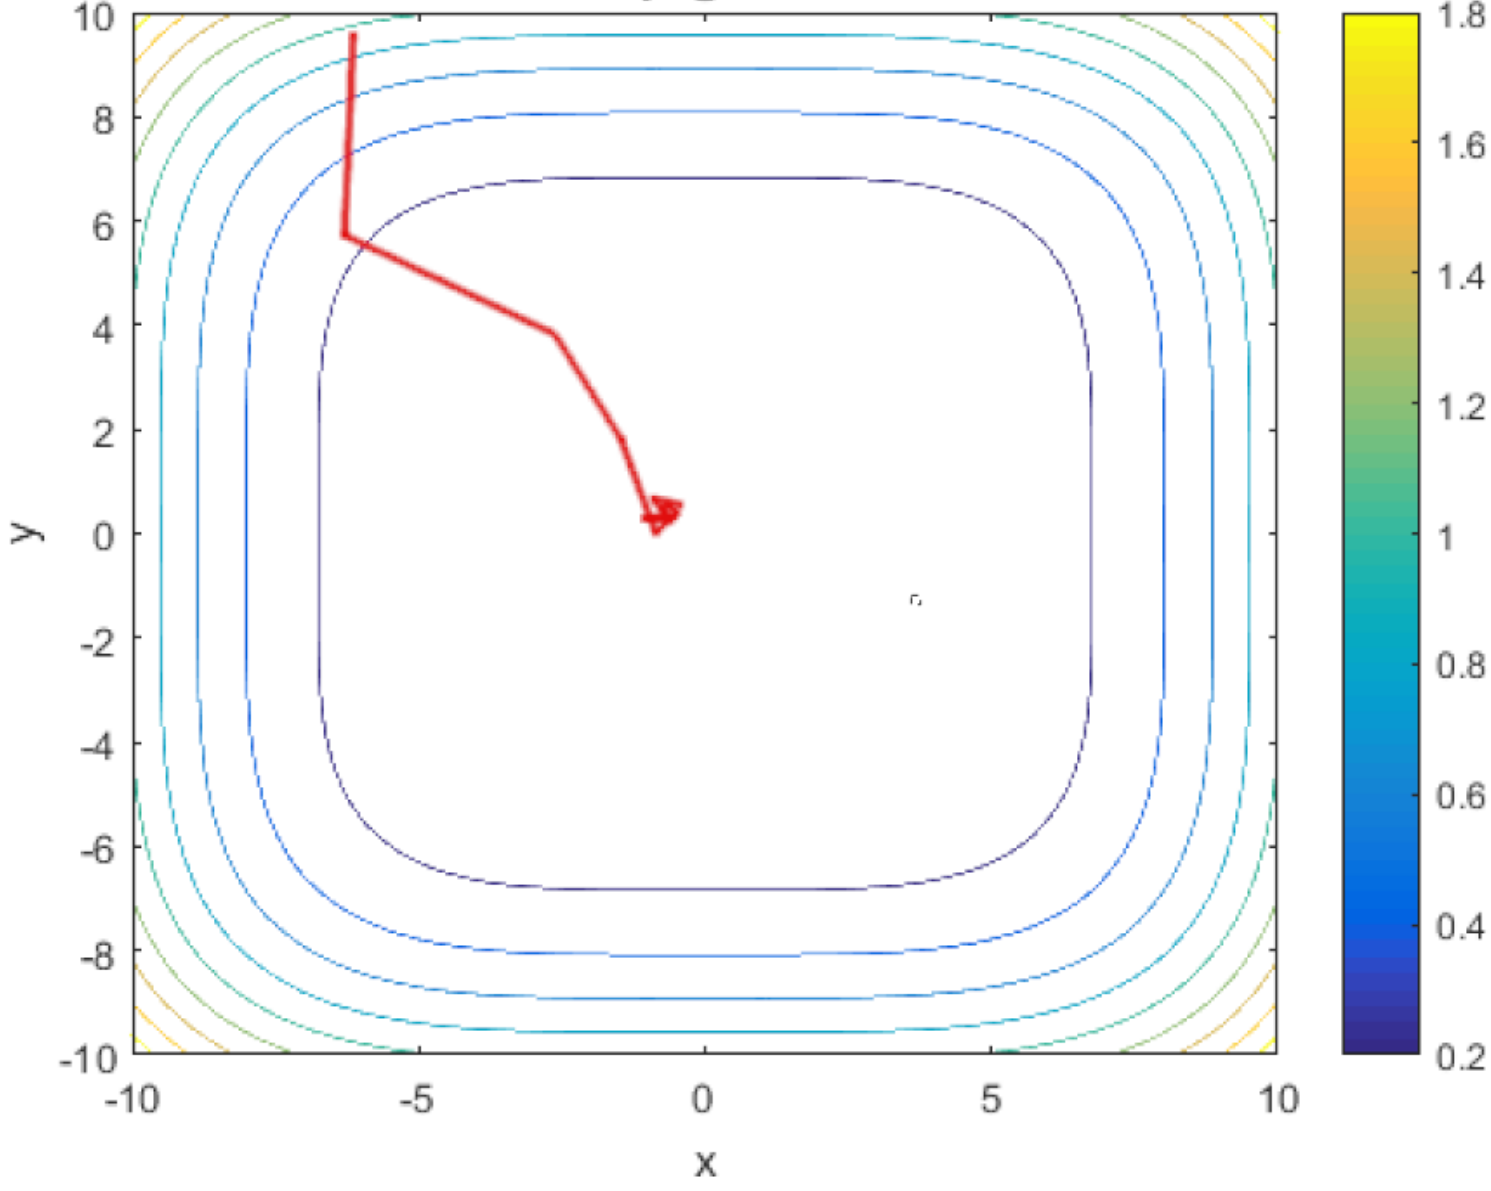
\includegraphics[width=37mm]{qingb.png}}
%   \\
%   \subfloat[Branin-A]{\label{figur:11}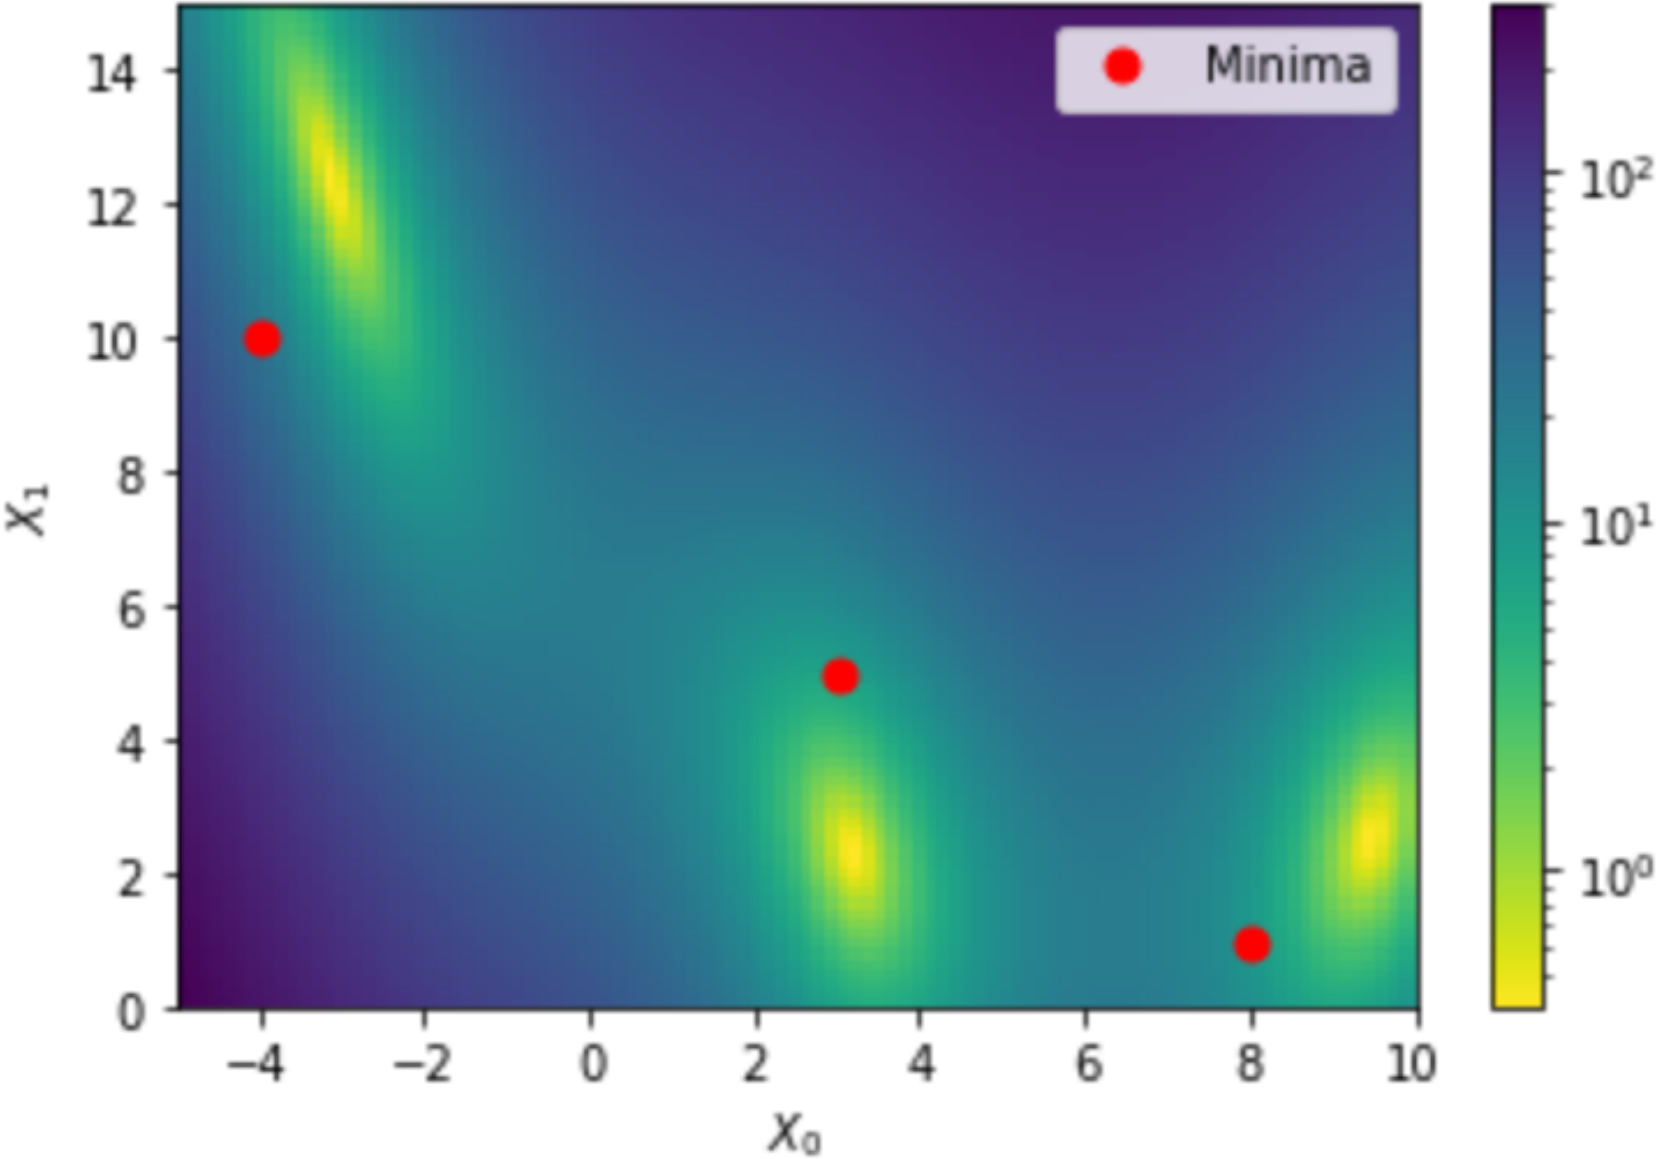
\includegraphics[width=45mm]{branina.png}}
%   \subfloat[Branin-B]{\label{figur:12}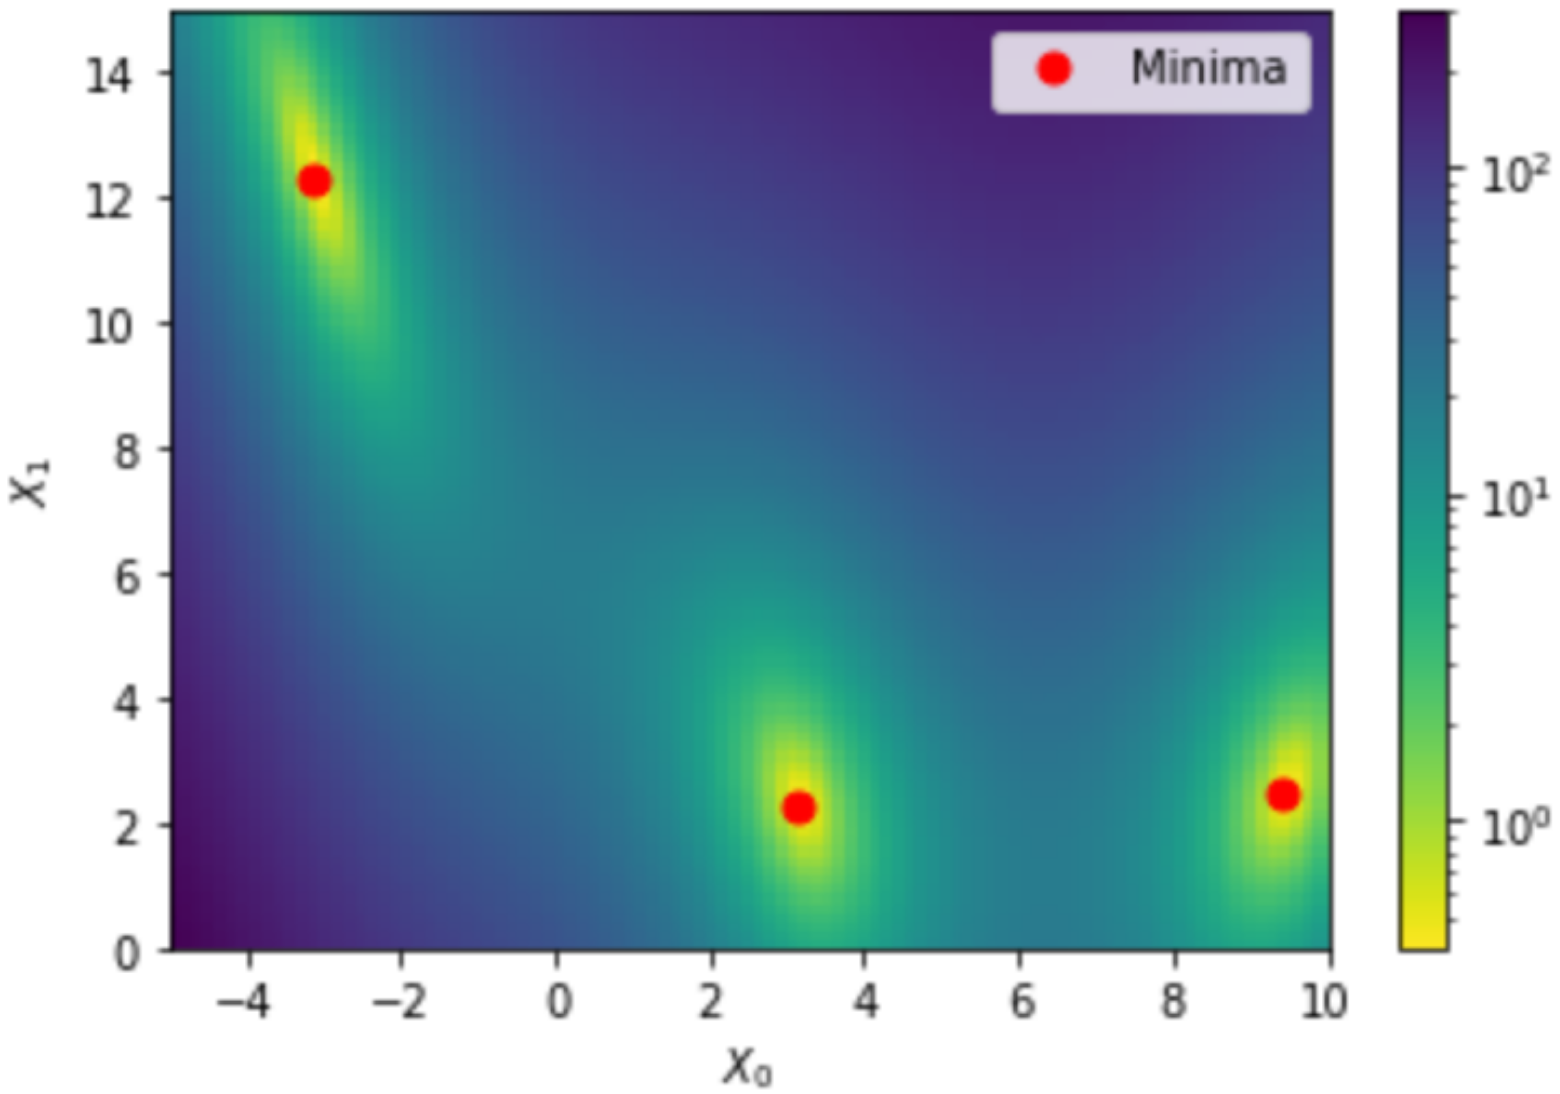
\includegraphics[width=45mm]{braninb.png}}
% \end{figure}

% \begin{figure*}[!t]
% \begin{subfigure}{.275\textwidth}
%   \centering
%   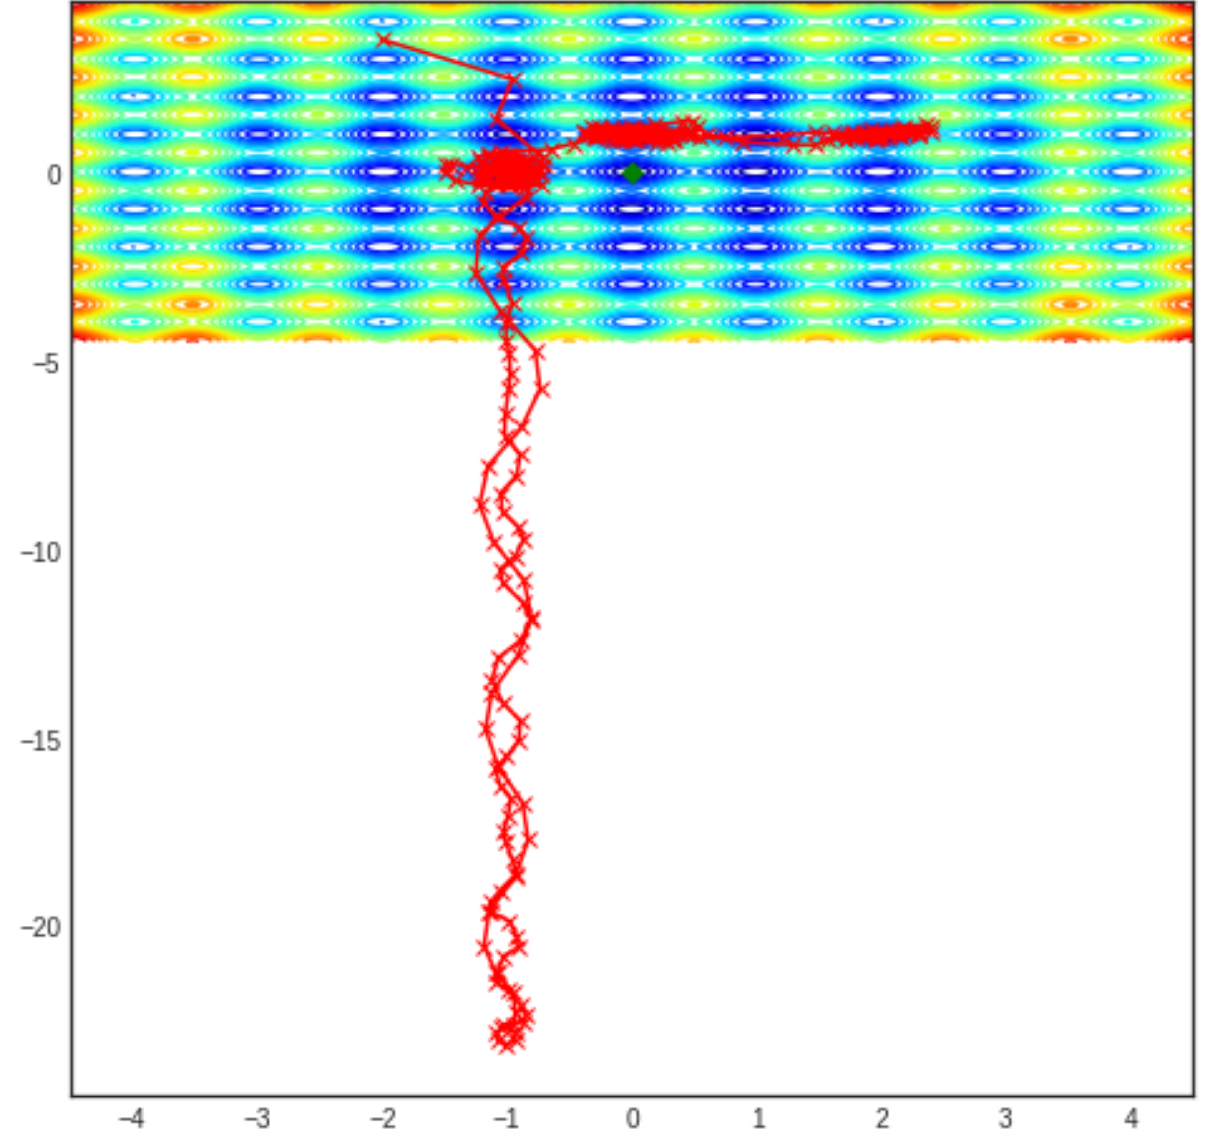
\includegraphics[width=0.14\paperwidth]{rastrigina.png}
%   \caption{Rastrigin-A}
%   \label{fig:figur:13}
% \end{subfigure}%
% \begin{subfigure}{.275\textwidth}
%   \centering
%   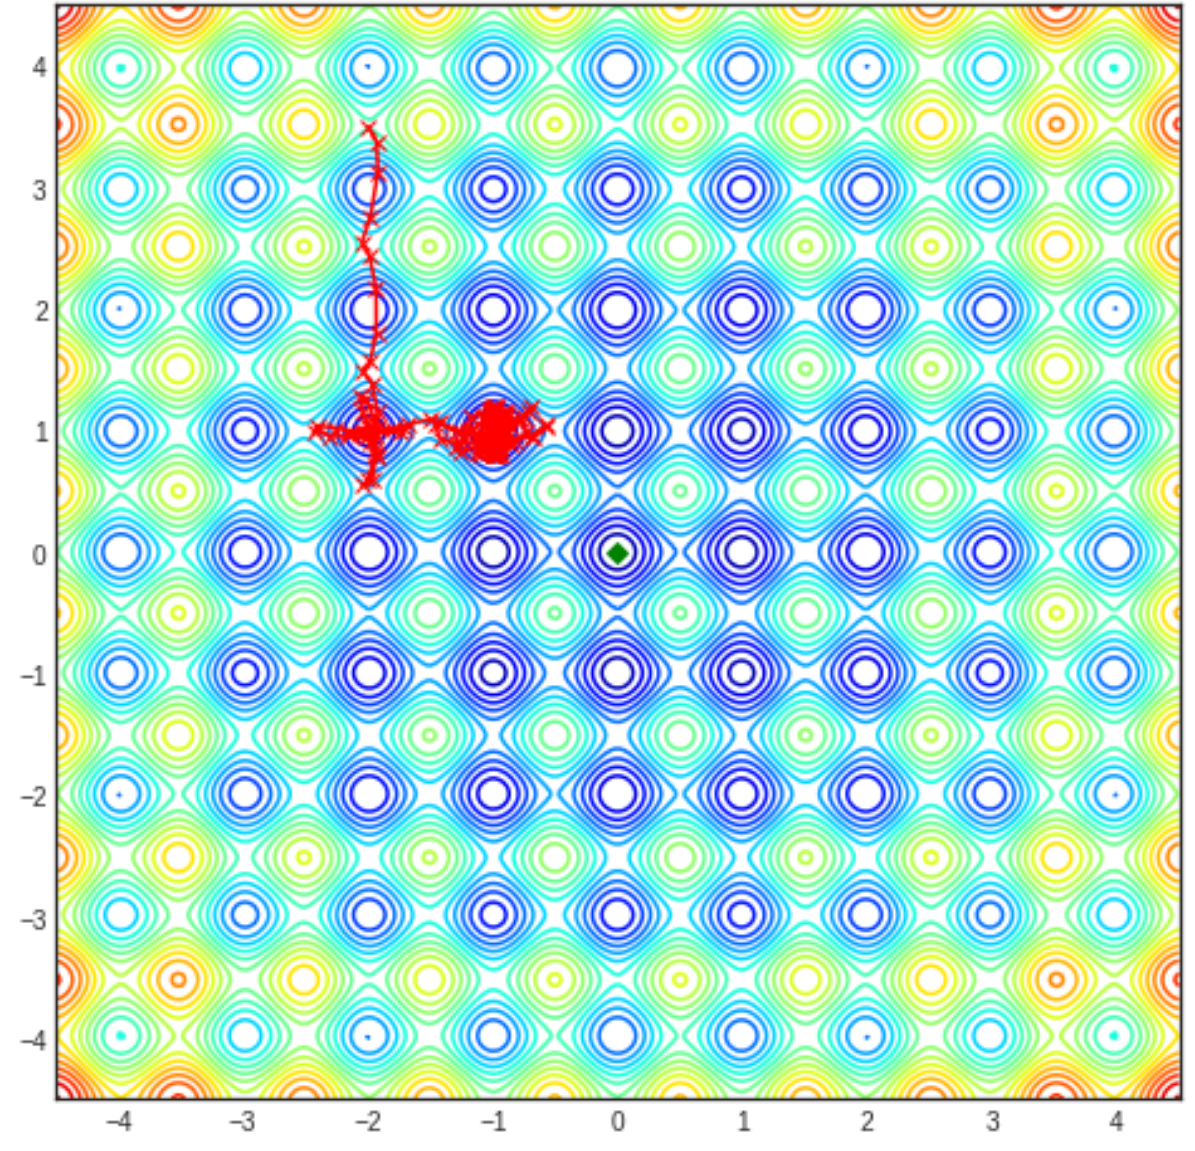
\includegraphics[width=0.14\paperwidth]{rastriginb.png}
%   \caption{Rastrigin-B}
%   \label{fig:figur:14}
% \end{subfigure}
% \begin{subfigure}{.275\textwidth}
%   \centering
%   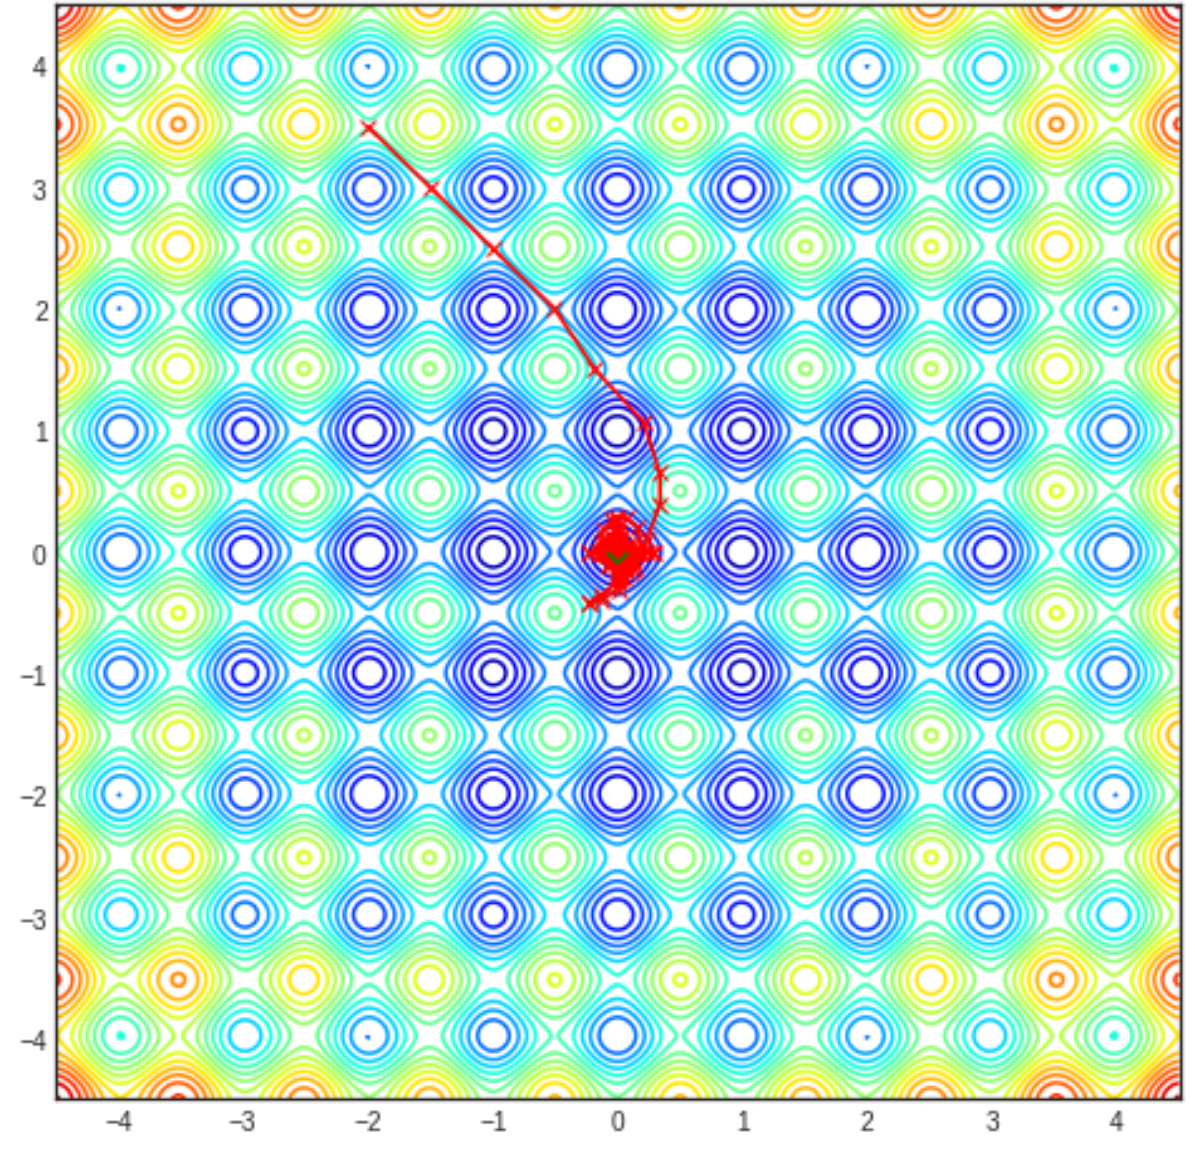
\includegraphics[width=0.14\paperwidth]{rastriginc.png}
%   \caption{Rastrigin-C}
%   \label{fig:figur:15}
% \end{subfigure}%
% \begin{subfigure}{.275\textwidth}
%   \centering
%   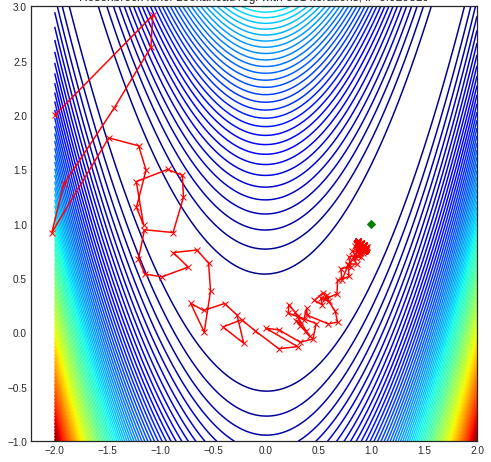
\includegraphics[width=0.14\paperwidth]{rosenbrocka.png}
%   \caption{Rosenbrock-A}
%   \label{fig:figur:16}
% \end{subfigure}
% \begin{subfigure}{.275\textwidth}
%   \centering
%   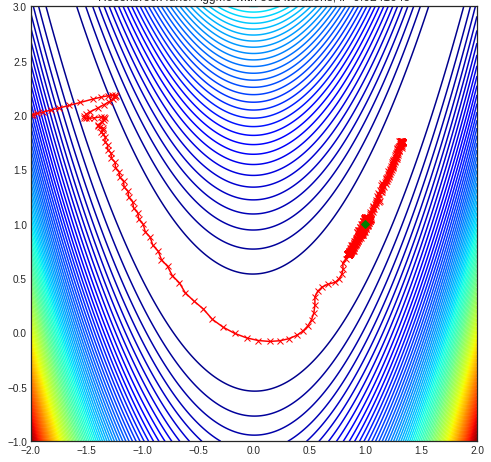
\includegraphics[width=0.14\paperwidth]{rosenbrockb.png}
%   \caption{Rosenbrock-B}
%   \label{fig:figur:17}
% \end{subfigure}%
% \begin{subfigure}{.275\textwidth}
%   \centering
%   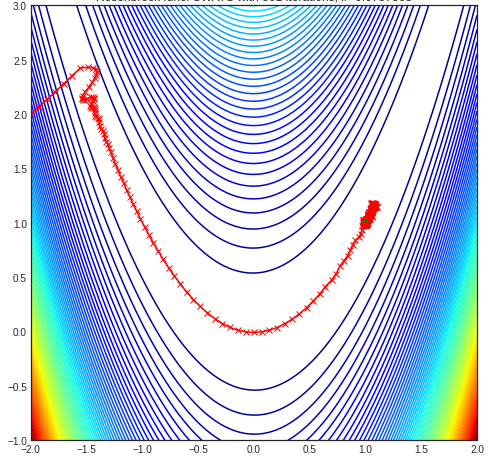
\includegraphics[width=0.14\paperwidth]{rosenbrockc.png}
%   \caption{Rosenbrock-C}
%   \label{fig:figur:18}
% \end{subfigure}
% \caption{Departmant C Dominance}
% \label{fig:sfig6}
% \end{figure*}

\begin{figure}[!t]
\begin{subfigure}{.275\textwidth}
  \centering
  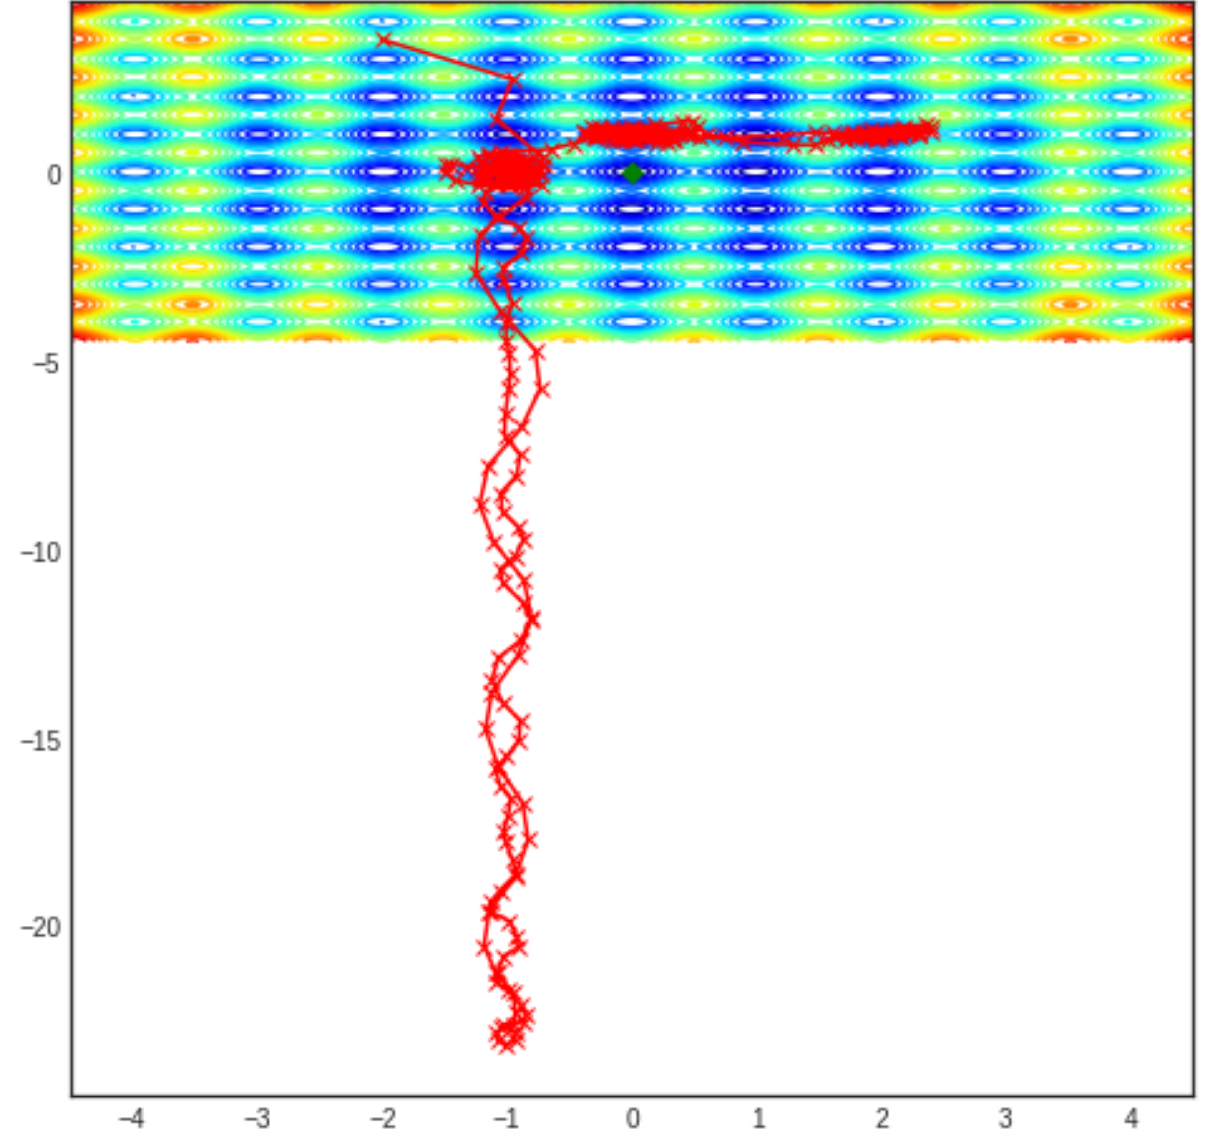
\includegraphics[width=.6\linewidth]{rastrigina.png}
  \caption{Rastrigin-A}
  \label{fig:figur:13}
\end{subfigure}%
\begin{subfigure}{.275\textwidth}
  \centering
  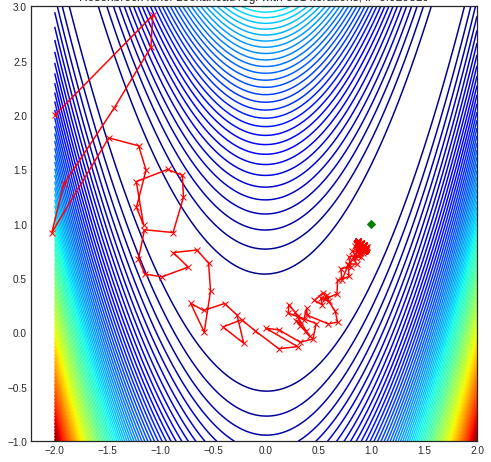
\includegraphics[width=.6\linewidth]{rosenbrocka.png}
  \caption{Rosenbrock-A}
  \label{fig:figur:14}
\end{subfigure}
\begin{subfigure}{.275\textwidth}
  \centering
  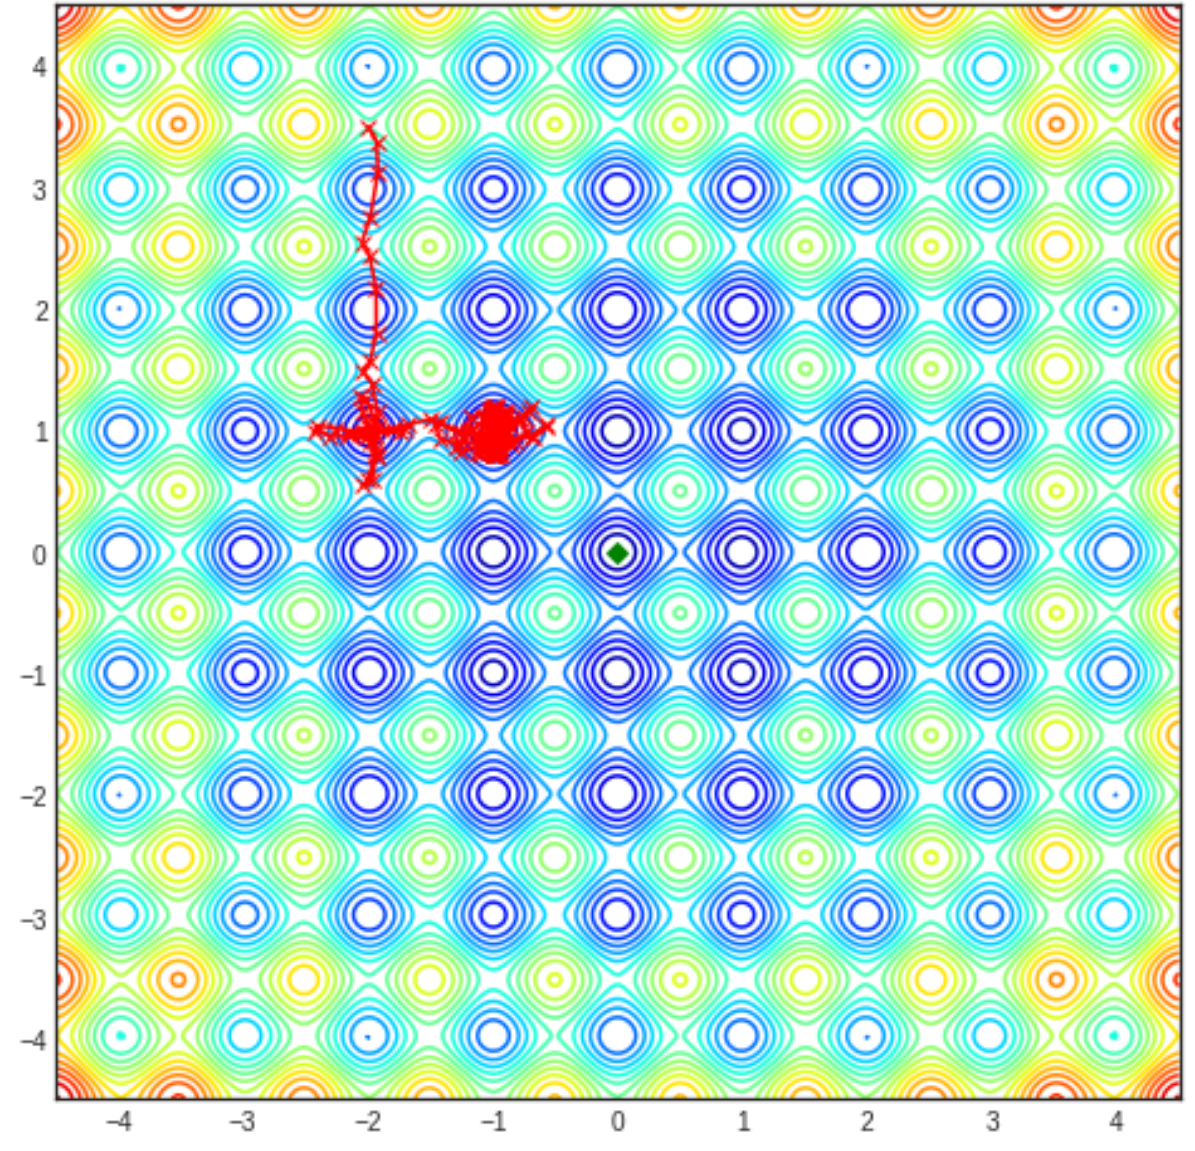
\includegraphics[width=.6\linewidth]{rastriginb.png}
  \caption{Rastrigin-B}
  \label{fig:figur:15}
\end{subfigure}%
\begin{subfigure}{.275\textwidth}
  \centering
  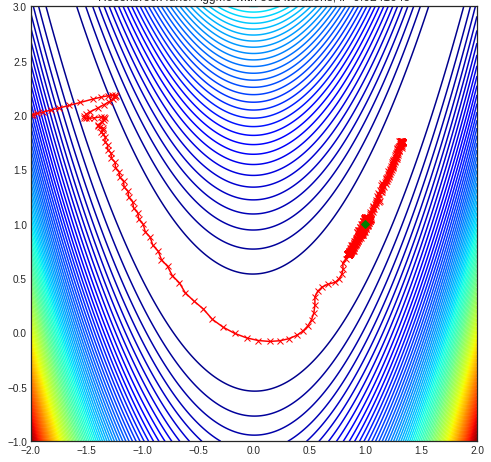
\includegraphics[width=.6\linewidth]{rosenbrockb.png}
  \caption{Rosenbrock-B}
  \label{fig:figur:16}
\end{subfigure}
\begin{subfigure}{.275\textwidth}
  \centering
  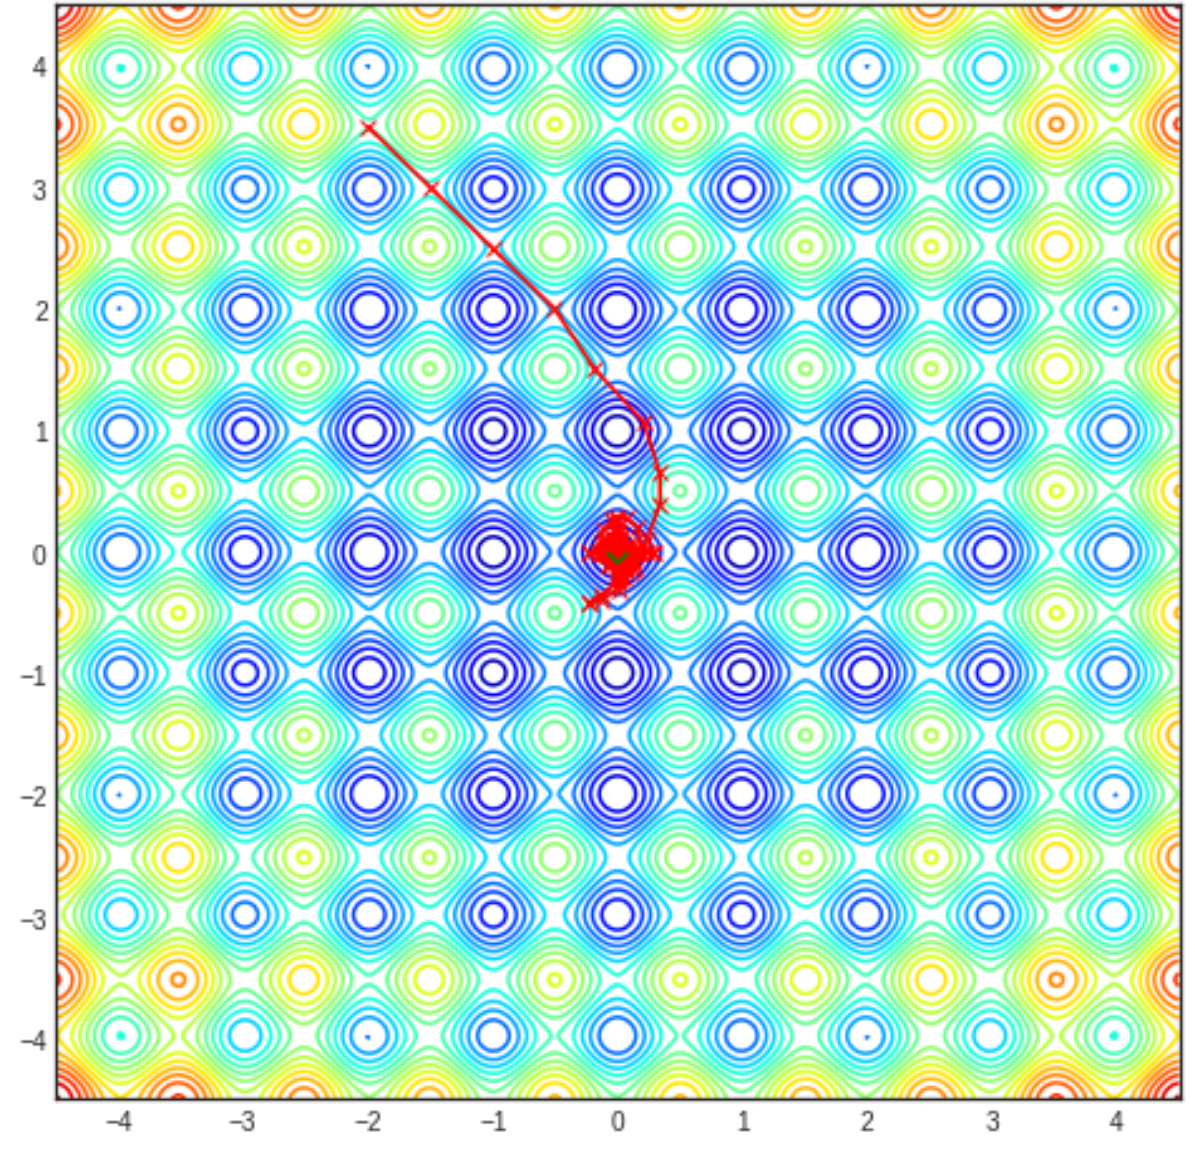
\includegraphics[width=.6\linewidth]{rastriginc.png}
  \caption{Rastrigin-C}
  \label{fig:figur:17}
\end{subfigure}%
\begin{subfigure}{.275\textwidth}
  \centering
  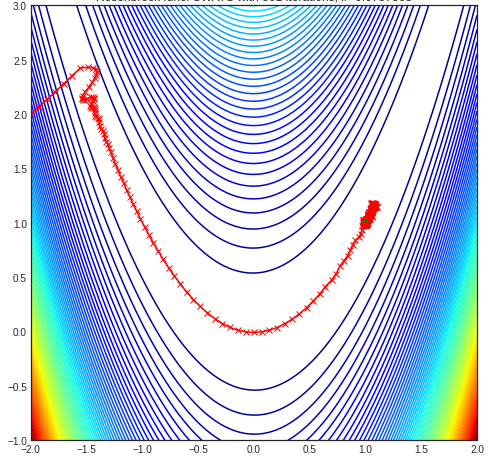
\includegraphics[width=.6\linewidth]{rosenbrockc.png}
  \caption{Rosenbrock-C}
  \label{fig:figur:18}
\end{subfigure}
\caption{Departmant C Dominance}
\label{fig:sfig6}
\end{figure}


% \begin{figure*}[!t]
%   \centering
%   \label{figur}\caption{Department C Dominant}
% 
%   \subfloat[Alpine-A]{\label{figur:13}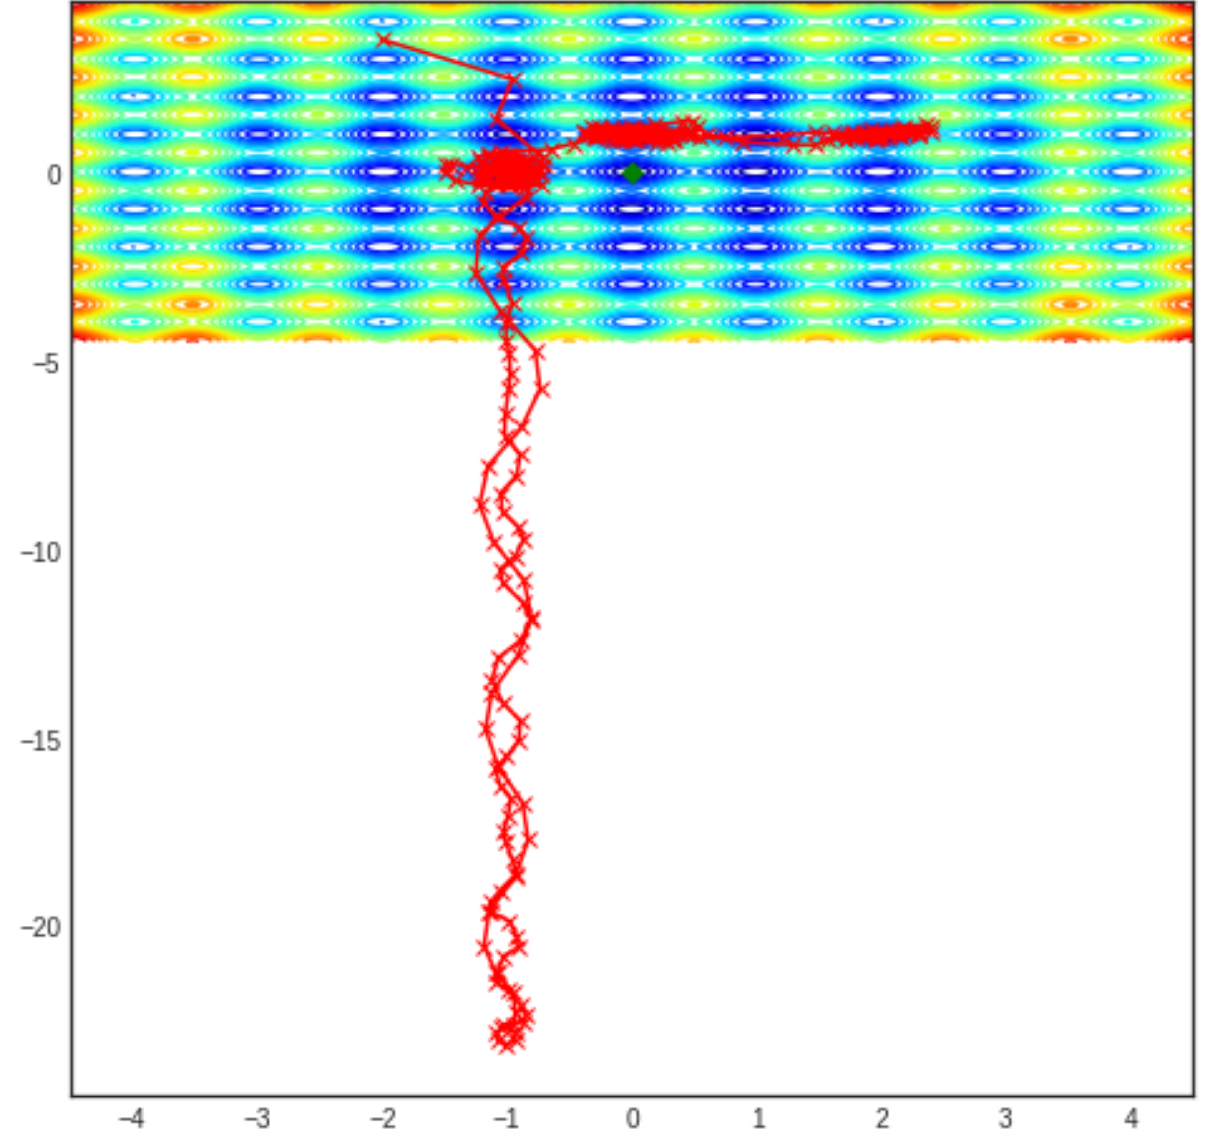
\includegraphics[width=45mm]{rastrigina.png}}
%   \subfloat[Alpine-B]{\label{figur:14}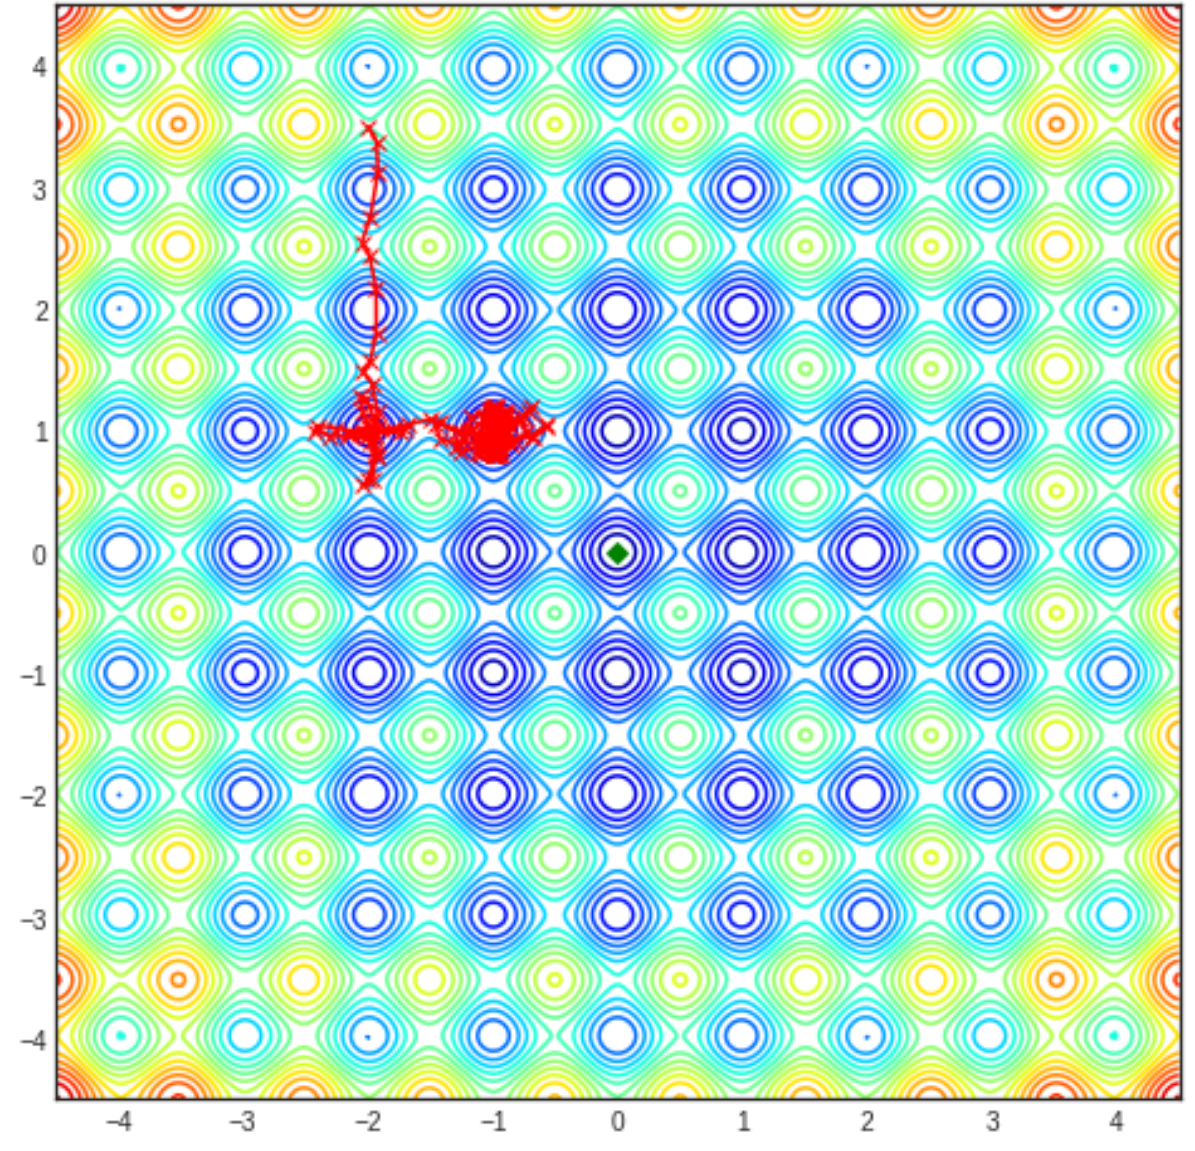
\includegraphics[width=45mm]{rastriginb.png}}
%   \subfloat[Alpine-B]{\label{figur:15}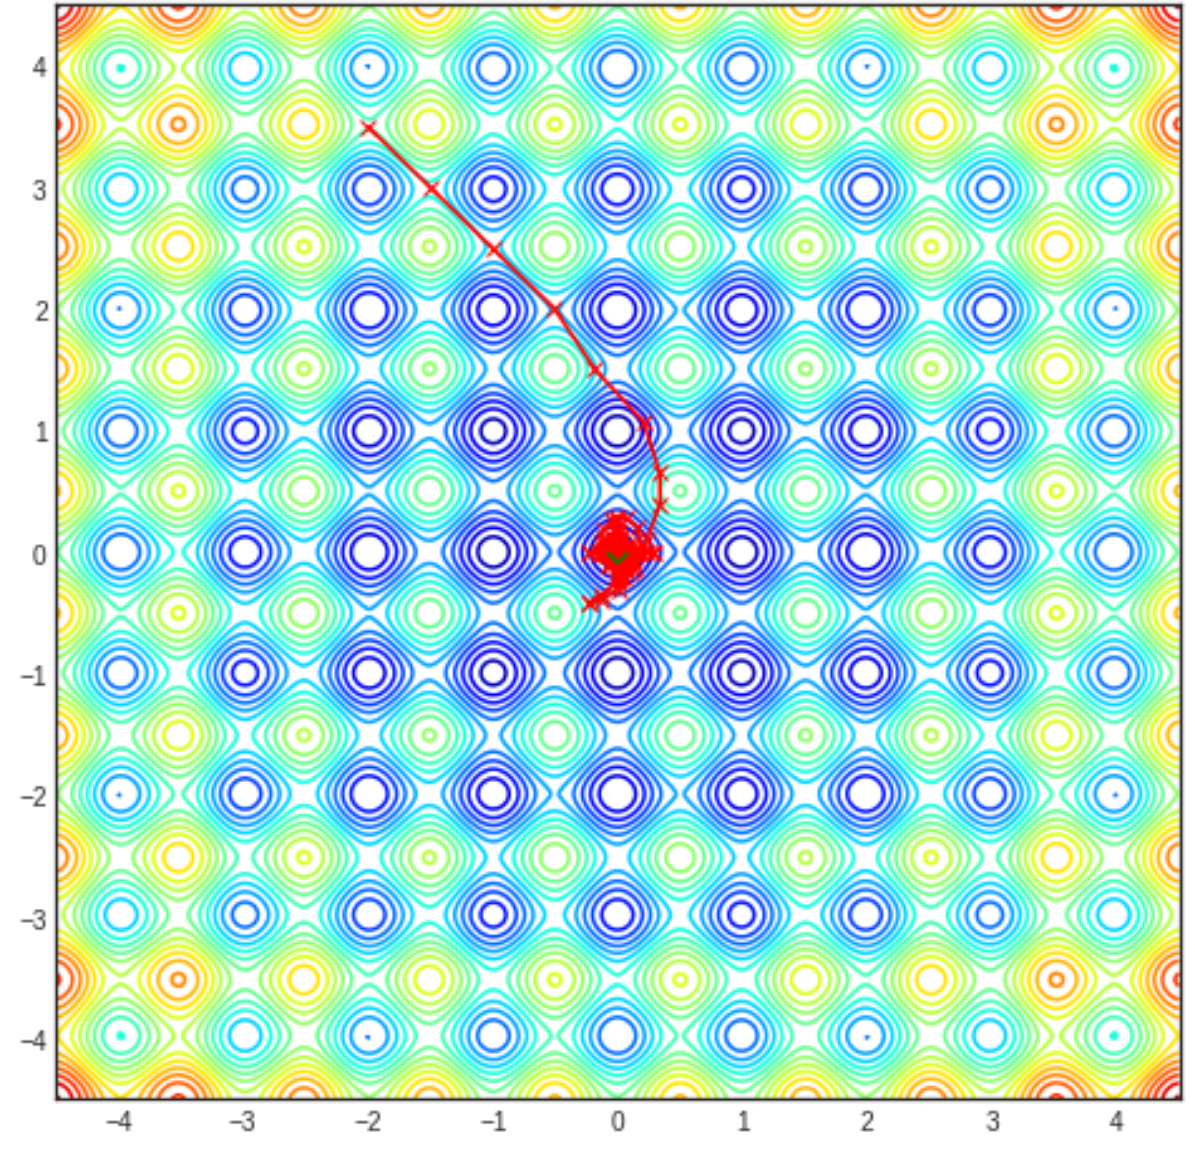
\includegraphics[width=45mm]{rastriginc.png}}
%   \\
%   \subfloat[Qing-A]{\label{figur:16}\includegraphics[width=45mm]{rosenbrocka.png}}
%   \subfloat[Qing-B]{\label{figur:17}\includegraphics[width=45mm]{rosenbrockb.png}}
%   \subfloat[Alpine-B]{\label{figur:18}\includegraphics[width=45mm]{rosenbrockc.png}}
%   \\
% \end{figure*}

\section{Conclusion and Future Work}

In this paper, we have presented Democratic Algorithm (DA), a social-construct-based algorithm which is heavily inspired by hierarchical swarm intelligence and real-life social establishments. The results presented cement the competence of DA as it outperforms other algorithms in multiple unimodal and multimodal landscapes. For any future extensions on this work, the following areas can be explored:

\begin{itemize}
\item Improved updation rules for the coefficient vectors.
\item Increase the number of parameters for improved model performance.
\item Generate a framework to decide on the number of departments.
\item Decrease the complexity of the algorithm by improving the table updation.
\item Introduction of concurrency.
\end{itemize}


\begin{thebibliography}{00}
\bibitem{chankong} Chankong V., Haimes Y, Thadathil J., Zionts S. (1985), Multiple Criteria Optimization: A State of the Art Review, Decision Making with Multiple Objectives, Lecture Notes in Economics and Mathematical Systems 242, Edited by Y.Y. Haimes, V. Chankong, SpringerVerlag, 36.

\bibitem{liu} H. Liu, F. Gu and Q. Zhang, "Decomposition of a Multiobjective Optimization Problem Into a Number of Simple Multiobjective Subproblems," in IEEE Transactions on Evolutionary Computation, vol. 18, no. 3, pp. 450-455, June 2014, doi: 10.1109/TEVC.2013.2281533. 

\bibitem{Deb} K. Deb, K. Miettinen and S. Chaudhuri, "Toward an Estimation of Nadir Objective Vector Using a Hybrid of Evolutionary and Local Search Approaches," in IEEE Transactions on Evolutionary Computation, vol. 14, no. 6, pp. 821-841, Dec. 2010, doi: 10.1109/TEVC.2010.2041667.

\bibitem{arora} Marler, R.T., Arora, J.S. The weighted sum method for multi-objective optimization: new insights. Struct Multidisc Optim 41, 853–862 (2010). https://doi.org/10.1007/s00158-009-0460-7

\bibitem{cooper} K. Cooper, S. R. Hunter and K. Nagaraj, "An epsilon-constraint method for integer-ordered bi-objective simulation optimization," 2017 Winter Simulation Conference (WSC), Las Vegas, NV, 2017, pp. 2303-2314, doi: 10.1109/WSC.2017.8247961.

\bibitem{ryu} N. Ryu, W. S. Song, Y. Jung and S. Min, "Multi-Objective Topology Optimization of a Magnetic Actuator Using an Adaptive Weight and Tunneling Method," in IEEE Transactions on Magnetics, vol. 55, no. 6, pp. 1-4, June 2019, Art no. 7202504, doi: 10.1109/TMAG.2019.2899893.

\bibitem{sinha} A. Sinha, K. Deb, P. Korhonen and J. Wallenius, "Progressively interactive evolutionary multi-objective optimization method using generalized polynomial value functions," IEEE Congress on Evolutionary Computation, Barcelona, 2010, pp. 1-8, doi: 10.1109/CEC.2010.5586278.

\bibitem{kim} J. Kim, J. Han, Y. Kim, S. Choi and E. Kim, "Preference-Based Solution Selection Algorithm for Evolutionary Multiobjective Optimization," in IEEE Transactions on Evolutionary Computation, vol. 16, no. 1, pp. 20-34, Feb. 2012, doi: 10.1109/TEVC.2010.2098412.

\bibitem{an} S. An, S. Yang and Z. Ren, "Incorporating Light Beam Search in a Vector Normal Boundary Intersection Method for Linear Antenna Array Optimization," in IEEE Transactions on Magnetics, vol. 53, no. 6, pp. 1-4, June 2017, Art no. 7001304, doi: 10.1109/TMAG.2017.2664077.

\bibitem{lim} P. Limbourg and D. E. S. Aponte, "An optimization algorithm for imprecise multi-objective problem functions," 2005 IEEE Congress on Evolutionary Computation, Edinburgh, Scotland, 2005, pp. 459-466 Vol.1, doi: 10.1109/CEC.2005.1554719.

\bibitem{conv} G. Rudolph and A. Agapie, "Convergence properties of some multi-objective evolutionary algorithms," Proceedings of the 2000 Congress on Evolutionary Computation. CEC00 (Cat. No.00TH8512), La Jolla, CA, USA, 2000, pp. 1010-1016 vol.2, doi: 10.1109/CEC.2000.870756.

\bibitem{arnold} D. V. Arnold and R. Salomon, "Evolutionary Gradient Search Revisited," in IEEE Transactions on Evolutionary Computation, vol. 11, no. 4, pp. 480-495, Aug. 2007, doi: 10.1109/TEVC.2006.882427.

\bibitem{vikhar} P. A. Vikhar, "Evolutionary algorithms: A critical review and its future prospects," 2016 International Conference on Global Trends in Signal Processing, Information Computing and Communication (ICGTSPICC), Jalgaon, 2016, pp. 261-265, doi: 10.1109/ICGTSPICC.2016.7955308.

\bibitem{swarm} Yan-fei Zhu and Xiong-min Tang, "Overview of swarm intelligence," 2010 International Conference on Computer Application and System Modeling (ICCASM 2010), Taiyuan, 2010, pp. V9-400-V9-403, doi: 10.1109/ICCASM.2010.5623005.

\bibitem{man} K. F. Man, K. S. Tang and S. Kwong, "Genetic algorithms: concepts and applications [in engineering design]," in IEEE Transactions on Industrial Electronics, vol. 43, no. 5, pp. 519-534, Oct. 1996, doi: 10.1109/41.538609.

\bibitem{abdul} W. Abdulal, O. A. Jadaan, A. Jabas, S. Ramachandram, M. Kaiiali and C. R. Rao, "Rank-Based Genetic Algorithm with Limited Iteration for Grid Scheduling," 2009 First ICCICSN, Indore, 2009, pp. 29-34, doi: 10.1109/CICSYN.2009.23.

\bibitem{kita} M. Takahashi and H. Kita, "A crossover operator using independent component analysis for real-coded genetic algorithms," Proceedings of the 2001 Congress on Evolutionary Computation (IEEE Cat. No.01TH8546), Seoul, South Korea, 2001, pp. 643-649 vol. 1, doi: 10.1109/CEC.2001.934452.

\bibitem{im} X. Deng, "Application of Adaptive Genetic Algorithm in Inversion Analysis of Permeability Coefficients," 2008 Second International Conference on Genetic and Evolutionary Computing, Hubei, 2008, pp. 61-65, doi: 10.1109/WGEC.2008.63.

\bibitem{pso} J. Kennedy and R. Eberhart, "Particle swarm optimization," Proceedings of ICNN'95 - International Conference on Neural Networks, Perth, WA, Australia, 1995, pp. 1942-1948 vol.4, doi: 10.1109/ICNN.1995.488968.

\bibitem{gwo} D. Jitkongchuen, P. Phaidang and P. Pongtawevirat, "Grey wolf optimization algorithm with invasion-based migration operation," 2016 IEEE/ACIS 15th International Conference on Computer and Information Science (ICIS), Okayama, 2016, pp. 1-5, doi: 10.1109/ICIS.2016.7550769.

\bibitem{mvo} H. Jia, X. Peng, W. Song, C. Lang, Z. Xing and K. Sun, "Multiverse Optimization Algorithm Based on Lévy Flight Improvement for Multithreshold Color Image Segmentation," in IEEE Access, vol. 7, pp. 32805-32844, 2019, doi: 10.1109/ACCESS.2019.2903345.

\bibitem{cs} M. Naik, M. R. Nath, A. Wunnava, S. Sahany and R. Panda, "A new adaptive Cuckoo search algorithm," 2015 IEEE 2nd International Conference on Recent Trends in Information Systems (ReTIS), Kolkata, 2015, pp. 1-5, doi: 10.1109/ReTIS.2015.7232842.

\bibitem{bf} R. W. Garden and A. P. Engelbrecht, "Analysis and classification of optimisation benchmark functions and benchmark suites," 2014 IEEE Congress on Evolutionary Computation (CEC), Beijing, 2014, pp. 1641-1649, doi: 10.1109/CEC.2014.6900240.

\end{thebibliography}


% \begin{thebibliography}{00}
% \bibitem{b1} G. Eason, B. Noble, and I. N. Sneddon, ``On certain integrals of Lipschitz-Hankel type involving products of Bessel functions,'' Phil. Trans. Roy. Soc. London, vol. A247, pp. 529--551, April 1955.
% \bibitem{b2} J. Clerk Maxwell, A Treatise on Electricity and Magnetism, 3rd ed., vol. 2. Oxford: Clarendon, 1892, pp.68--73.
% \bibitem{b3} I. S. Jacobs and C. P. Bean, ``Fine particles, thin films and exchange anisotropy,'' in Magnetism, vol. III, G. T. Rado and H. Suhl, Eds. New York: Academic, 1963, pp. 271--350.
% \bibitem{b4} K. Elissa, ``Title of paper if known,'' unpublished.
% \bibitem{b5} R. Nicole, ``Title of paper with only first word capitalized,'' J. Name Stand. Abbrev., in press.
% \bibitem{b6} Y. Yorozu, M. Hirano, K. Oka, and Y. Tagawa, ``Electron spectroscopy studies on magneto-optical media and plastic substrate interface,'' IEEE Transl. J. Magn. Japan, vol. 2, pp. 740--741, August 1987 [Digests 9th Annual Conf. Magnetics Japan, p. 301, 1982].
% \bibitem{b7} M. Young, The Technical Writer's Handbook. Mill Valley, CA: University Science, 1989.
% \end{thebibliography}
% \vspace{12pt}
% \color{red}
% IEEE conference templates contain guidance text for composing and formatting conference papers. Please ensure that all template text is removed from your conference paper prior to submission to the conference. Failure to remove the template text from your paper may result in your paper not being published.

\end{document}
